\documentclass[twoside]{book}

% Packages required by doxygen
\usepackage{calc}
\usepackage{doxygen}
\usepackage{graphicx}
\usepackage[utf8]{inputenc}
\usepackage{makeidx}
\usepackage{multicol}
\usepackage{multirow}
\usepackage{fixltx2e}
\PassOptionsToPackage{warn}{textcomp}
\usepackage{textcomp}
\usepackage[nointegrals]{wasysym}
\usepackage[table]{xcolor}

% Font selection
\usepackage[T1]{fontenc}
\usepackage{mathptmx}
\usepackage[scaled=.90]{helvet}
\usepackage{courier}
\usepackage{amssymb}
\usepackage{sectsty}
\renewcommand{\familydefault}{\sfdefault}
\allsectionsfont{%
  \fontseries{bc}\selectfont%
  \color{darkgray}%
}
\renewcommand{\DoxyLabelFont}{%
  \fontseries{bc}\selectfont%
  \color{darkgray}%
}
\newcommand{\+}{\discretionary{\mbox{\scriptsize$\hookleftarrow$}}{}{}}

% Page & text layout
\usepackage{geometry}
\geometry{%
  a4paper,%
  top=2.5cm,%
  bottom=2.5cm,%
  left=2.5cm,%
  right=2.5cm%
}
\tolerance=750
\hfuzz=15pt
\hbadness=750
\setlength{\emergencystretch}{15pt}
\setlength{\parindent}{0cm}
\setlength{\parskip}{0.2cm}
\makeatletter
\renewcommand{\paragraph}{%
  \@startsection{paragraph}{4}{0ex}{-1.0ex}{1.0ex}{%
    \normalfont\normalsize\bfseries\SS@parafont%
  }%
}
\renewcommand{\subparagraph}{%
  \@startsection{subparagraph}{5}{0ex}{-1.0ex}{1.0ex}{%
    \normalfont\normalsize\bfseries\SS@subparafont%
  }%
}
\makeatother

% Headers & footers
\usepackage{fancyhdr}
\pagestyle{fancyplain}
\fancyhead[LE]{\fancyplain{}{\bfseries\thepage}}
\fancyhead[CE]{\fancyplain{}{}}
\fancyhead[RE]{\fancyplain{}{\bfseries\leftmark}}
\fancyhead[LO]{\fancyplain{}{\bfseries\rightmark}}
\fancyhead[CO]{\fancyplain{}{}}
\fancyhead[RO]{\fancyplain{}{\bfseries\thepage}}
\fancyfoot[LE]{\fancyplain{}{}}
\fancyfoot[CE]{\fancyplain{}{}}
\fancyfoot[RE]{\fancyplain{}{\bfseries\scriptsize Generated on Tue Dec 23 2014 20\+:19\+:46 for Simple\+R\+P\+G by Doxygen }}
\fancyfoot[LO]{\fancyplain{}{\bfseries\scriptsize Generated on Tue Dec 23 2014 20\+:19\+:46 for Simple\+R\+P\+G by Doxygen }}
\fancyfoot[CO]{\fancyplain{}{}}
\fancyfoot[RO]{\fancyplain{}{}}
\renewcommand{\footrulewidth}{0.4pt}
\renewcommand{\chaptermark}[1]{%
  \markboth{#1}{}%
}
\renewcommand{\sectionmark}[1]{%
  \markright{\thesection\ #1}%
}

% Indices & bibliography
\usepackage{natbib}
\usepackage[titles]{tocloft}
\setcounter{tocdepth}{3}
\setcounter{secnumdepth}{5}
\makeindex

% Hyperlinks (required, but should be loaded last)
\usepackage{ifpdf}
\ifpdf
  \usepackage[pdftex,pagebackref=true]{hyperref}
\else
  \usepackage[ps2pdf,pagebackref=true]{hyperref}
\fi
\hypersetup{%
  colorlinks=true,%
  linkcolor=blue,%
  citecolor=blue,%
  unicode%
}

% Custom commands
\newcommand{\clearemptydoublepage}{%
  \newpage{\pagestyle{empty}\cleardoublepage}%
}


%===== C O N T E N T S =====

\begin{document}

% Titlepage & ToC
\hypersetup{pageanchor=false,
             bookmarks=true,
             bookmarksnumbered=true,
             pdfencoding=unicode
            }
\pagenumbering{roman}
\begin{titlepage}
\vspace*{7cm}
\begin{center}%
{\Large Simple\+R\+P\+G }\\
\vspace*{1cm}
{\large Generated by Doxygen 1.8.7}\\
\vspace*{0.5cm}
{\small Tue Dec 23 2014 20:19:46}\\
\end{center}
\end{titlepage}
\clearemptydoublepage
\tableofcontents
\clearemptydoublepage
\pagenumbering{arabic}
\hypersetup{pageanchor=true}

%--- Begin generated contents ---
\chapter{Namespace Index}
\section{Namespace List}
Here is a list of all documented namespaces with brief descriptions\-:\begin{DoxyCompactList}
\item\contentsline{section}{\hyperlink{namespace_simple_r_p_g}{Simple\-R\-P\-G} }{\pageref{namespace_simple_r_p_g}}{}
\item\contentsline{section}{\hyperlink{namespace_simple_r_p_g_1_1_events}{Simple\-R\-P\-G.\-Events} }{\pageref{namespace_simple_r_p_g_1_1_events}}{}
\item\contentsline{section}{\hyperlink{namespace_simple_r_p_g_1_1_items}{Simple\-R\-P\-G.\-Items} }{\pageref{namespace_simple_r_p_g_1_1_items}}{}
\item\contentsline{section}{\hyperlink{namespace_simple_r_p_g_1_1_states}{Simple\-R\-P\-G.\-States} }{\pageref{namespace_simple_r_p_g_1_1_states}}{}
\item\contentsline{section}{\hyperlink{namespace_simple_r_p_g_1_1_widgets}{Simple\-R\-P\-G.\-Widgets} }{\pageref{namespace_simple_r_p_g_1_1_widgets}}{}
\item\contentsline{section}{\hyperlink{namespace_simple_r_p_g_1_1_windows}{Simple\-R\-P\-G.\-Windows} }{\pageref{namespace_simple_r_p_g_1_1_windows}}{}
\end{DoxyCompactList}

\chapter{Hierarchical Index}
\section{Class Hierarchy}
This inheritance list is sorted roughly, but not completely, alphabetically\+:\begin{DoxyCompactList}
\item \contentsline{section}{Simple\+R\+P\+G.\+Animation}{\pageref{class_simple_r_p_g_1_1_animation}}{}
\item \contentsline{section}{Simple\+R\+P\+G.\+Battler}{\pageref{class_simple_r_p_g_1_1_battler}}{}
\begin{DoxyCompactList}
\item \contentsline{section}{Simple\+R\+P\+G.\+A\+I\+Battler}{\pageref{class_simple_r_p_g_1_1_a_i_battler}}{}
\item \contentsline{section}{Simple\+R\+P\+G.\+Player\+Battler}{\pageref{class_simple_r_p_g_1_1_player_battler}}{}
\end{DoxyCompactList}
\item \contentsline{section}{Simple\+R\+P\+G.\+Drawable}{\pageref{class_simple_r_p_g_1_1_drawable}}{}
\begin{DoxyCompactList}
\item \contentsline{section}{Simple\+R\+P\+G.\+Camera}{\pageref{class_simple_r_p_g_1_1_camera}}{}
\item \contentsline{section}{Simple\+R\+P\+G.\+States.\+Game\+State}{\pageref{class_simple_r_p_g_1_1_states_1_1_game_state}}{}
\begin{DoxyCompactList}
\item \contentsline{section}{Simple\+R\+P\+G.\+States.\+Battle\+Action\+Select\+State}{\pageref{class_simple_r_p_g_1_1_states_1_1_battle_action_select_state}}{}
\item \contentsline{section}{Simple\+R\+P\+G.\+States.\+Battle\+State}{\pageref{class_simple_r_p_g_1_1_states_1_1_battle_state}}{}
\item \contentsline{section}{Simple\+R\+P\+G.\+States.\+Inventory\+State}{\pageref{class_simple_r_p_g_1_1_states_1_1_inventory_state}}{}
\item \contentsline{section}{Simple\+R\+P\+G.\+States.\+Map\+State}{\pageref{class_simple_r_p_g_1_1_states_1_1_map_state}}{}
\item \contentsline{section}{Simple\+R\+P\+G.\+States.\+Message\+State}{\pageref{class_simple_r_p_g_1_1_states_1_1_message_state}}{}
\item \contentsline{section}{Simple\+R\+P\+G.\+States.\+Pause\+State}{\pageref{class_simple_r_p_g_1_1_states_1_1_pause_state}}{}
\item \contentsline{section}{Simple\+R\+P\+G.\+States.\+Target\+Select\+State}{\pageref{class_simple_r_p_g_1_1_states_1_1_target_select_state}}{}
\item \contentsline{section}{Simple\+R\+P\+G.\+States.\+Use\+Item\+State}{\pageref{class_simple_r_p_g_1_1_states_1_1_use_item_state}}{}
\end{DoxyCompactList}
\item \contentsline{section}{Simple\+R\+P\+G.\+Tile\+Map}{\pageref{class_simple_r_p_g_1_1_tile_map}}{}
\item \contentsline{section}{Simple\+R\+P\+G.\+Windows.\+Window}{\pageref{class_simple_r_p_g_1_1_windows_1_1_window}}{}
\begin{DoxyCompactList}
\item \contentsline{section}{Simple\+R\+P\+G.\+Windows.\+Item\+Description\+Window}{\pageref{class_simple_r_p_g_1_1_windows_1_1_item_description_window}}{}
\item \contentsline{section}{Simple\+R\+P\+G.\+Windows.\+List\+Box}{\pageref{class_simple_r_p_g_1_1_windows_1_1_list_box}}{}
\begin{DoxyCompactList}
\item \contentsline{section}{Simple\+R\+P\+G.\+Windows.\+Item\+List}{\pageref{class_simple_r_p_g_1_1_windows_1_1_item_list}}{}
\item \contentsline{section}{Simple\+R\+P\+G.\+Windows.\+Pause\+Window}{\pageref{class_simple_r_p_g_1_1_windows_1_1_pause_window}}{}
\item \contentsline{section}{Simple\+R\+P\+G.\+Windows.\+Use\+Item\+Window}{\pageref{class_simple_r_p_g_1_1_windows_1_1_use_item_window}}{}
\end{DoxyCompactList}
\item \contentsline{section}{Simple\+R\+P\+G.\+Windows.\+Message\+Window}{\pageref{class_simple_r_p_g_1_1_windows_1_1_message_window}}{}
\item \contentsline{section}{Simple\+R\+P\+G.\+Windows.\+Player\+Battle\+Status\+Window}{\pageref{class_simple_r_p_g_1_1_windows_1_1_player_battle_status_window}}{}
\end{DoxyCompactList}
\end{DoxyCompactList}
\item \contentsline{section}{Simple\+R\+P\+G.\+Drawable\+Layer}{\pageref{class_simple_r_p_g_1_1_drawable_layer}}{}
\begin{DoxyCompactList}
\item \contentsline{section}{Simple\+R\+P\+G.\+Object\+Layer}{\pageref{class_simple_r_p_g_1_1_object_layer}}{}
\item \contentsline{section}{Simple\+R\+P\+G.\+Tile\+Layer}{\pageref{class_simple_r_p_g_1_1_tile_layer}}{}
\end{DoxyCompactList}
\item \contentsline{section}{Simple\+R\+P\+G.\+Enemy\+Manager}{\pageref{class_simple_r_p_g_1_1_enemy_manager}}{}
\item \contentsline{section}{Simple\+R\+P\+G.\+Events.\+Event}{\pageref{class_simple_r_p_g_1_1_events_1_1_event}}{}
\begin{DoxyCompactList}
\item \contentsline{section}{Simple\+R\+P\+G.\+Events.\+Message\+Event}{\pageref{class_simple_r_p_g_1_1_events_1_1_message_event}}{}
\end{DoxyCompactList}
\item Game\begin{DoxyCompactList}
\item \contentsline{section}{Simple\+R\+P\+G.\+Game1}{\pageref{class_simple_r_p_g_1_1_game1}}{}
\end{DoxyCompactList}
\item I\+Comparable$<$ Map\+Object $>$\begin{DoxyCompactList}
\item \contentsline{section}{Simple\+R\+P\+G.\+Map\+Object}{\pageref{class_simple_r_p_g_1_1_map_object}}{}
\end{DoxyCompactList}
\item \contentsline{section}{Simple\+R\+P\+G.\+Input}{\pageref{class_simple_r_p_g_1_1_input}}{}
\item \contentsline{section}{Simple\+R\+P\+G.\+Item}{\pageref{class_simple_r_p_g_1_1_item}}{}
\item \contentsline{section}{Simple\+R\+P\+G.\+Item\+Container}{\pageref{class_simple_r_p_g_1_1_item_container}}{}
\item \contentsline{section}{Simple\+R\+P\+G.\+Item\+Manager}{\pageref{class_simple_r_p_g_1_1_item_manager}}{}
\item \contentsline{section}{Simple\+R\+P\+G.\+Player}{\pageref{class_simple_r_p_g_1_1_player}}{}
\item \contentsline{section}{Simple\+R\+P\+G.\+States.\+State\+Manager}{\pageref{class_simple_r_p_g_1_1_states_1_1_state_manager}}{}
\item \contentsline{section}{Simple\+R\+P\+G.\+Widgets.\+Text\+Widget}{\pageref{class_simple_r_p_g_1_1_widgets_1_1_text_widget}}{}
\item \contentsline{section}{Simple\+R\+P\+G.\+Tile}{\pageref{class_simple_r_p_g_1_1_tile}}{}
\end{DoxyCompactList}

\chapter{Class Index}
\section{Class List}
Here are the classes, structs, unions and interfaces with brief descriptions\+:\begin{DoxyCompactList}
\item\contentsline{section}{\hyperlink{class_simple_r_p_g_1_1_a_i_battler}{Simple\+R\+P\+G.\+A\+I\+Battler} }{\pageref{class_simple_r_p_g_1_1_a_i_battler}}{}
\item\contentsline{section}{\hyperlink{class_simple_r_p_g_1_1_animation}{Simple\+R\+P\+G.\+Animation} }{\pageref{class_simple_r_p_g_1_1_animation}}{}
\item\contentsline{section}{\hyperlink{class_simple_r_p_g_1_1_states_1_1_battle_action_select_state}{Simple\+R\+P\+G.\+States.\+Battle\+Action\+Select\+State} }{\pageref{class_simple_r_p_g_1_1_states_1_1_battle_action_select_state}}{}
\item\contentsline{section}{\hyperlink{class_simple_r_p_g_1_1_battler}{Simple\+R\+P\+G.\+Battler} }{\pageref{class_simple_r_p_g_1_1_battler}}{}
\item\contentsline{section}{\hyperlink{class_simple_r_p_g_1_1_states_1_1_battle_state}{Simple\+R\+P\+G.\+States.\+Battle\+State} }{\pageref{class_simple_r_p_g_1_1_states_1_1_battle_state}}{}
\item\contentsline{section}{\hyperlink{class_simple_r_p_g_1_1_camera}{Simple\+R\+P\+G.\+Camera} }{\pageref{class_simple_r_p_g_1_1_camera}}{}
\item\contentsline{section}{\hyperlink{class_simple_r_p_g_1_1_drawable}{Simple\+R\+P\+G.\+Drawable} }{\pageref{class_simple_r_p_g_1_1_drawable}}{}
\item\contentsline{section}{\hyperlink{class_simple_r_p_g_1_1_drawable_layer}{Simple\+R\+P\+G.\+Drawable\+Layer} }{\pageref{class_simple_r_p_g_1_1_drawable_layer}}{}
\item\contentsline{section}{\hyperlink{class_simple_r_p_g_1_1_enemy_manager}{Simple\+R\+P\+G.\+Enemy\+Manager} }{\pageref{class_simple_r_p_g_1_1_enemy_manager}}{}
\item\contentsline{section}{\hyperlink{class_simple_r_p_g_1_1_events_1_1_event}{Simple\+R\+P\+G.\+Events.\+Event} }{\pageref{class_simple_r_p_g_1_1_events_1_1_event}}{}
\item\contentsline{section}{\hyperlink{class_simple_r_p_g_1_1_game1}{Simple\+R\+P\+G.\+Game1} \\*This is the main type for your game }{\pageref{class_simple_r_p_g_1_1_game1}}{}
\item\contentsline{section}{\hyperlink{class_simple_r_p_g_1_1_states_1_1_game_state}{Simple\+R\+P\+G.\+States.\+Game\+State} }{\pageref{class_simple_r_p_g_1_1_states_1_1_game_state}}{}
\item\contentsline{section}{\hyperlink{class_simple_r_p_g_1_1_input}{Simple\+R\+P\+G.\+Input} }{\pageref{class_simple_r_p_g_1_1_input}}{}
\item\contentsline{section}{\hyperlink{class_simple_r_p_g_1_1_states_1_1_inventory_state}{Simple\+R\+P\+G.\+States.\+Inventory\+State} }{\pageref{class_simple_r_p_g_1_1_states_1_1_inventory_state}}{}
\item\contentsline{section}{\hyperlink{class_simple_r_p_g_1_1_item}{Simple\+R\+P\+G.\+Item} }{\pageref{class_simple_r_p_g_1_1_item}}{}
\item\contentsline{section}{\hyperlink{class_simple_r_p_g_1_1_item_container}{Simple\+R\+P\+G.\+Item\+Container} }{\pageref{class_simple_r_p_g_1_1_item_container}}{}
\item\contentsline{section}{\hyperlink{class_simple_r_p_g_1_1_windows_1_1_item_description_window}{Simple\+R\+P\+G.\+Windows.\+Item\+Description\+Window} }{\pageref{class_simple_r_p_g_1_1_windows_1_1_item_description_window}}{}
\item\contentsline{section}{\hyperlink{class_simple_r_p_g_1_1_windows_1_1_item_list}{Simple\+R\+P\+G.\+Windows.\+Item\+List} }{\pageref{class_simple_r_p_g_1_1_windows_1_1_item_list}}{}
\item\contentsline{section}{\hyperlink{class_simple_r_p_g_1_1_item_manager}{Simple\+R\+P\+G.\+Item\+Manager} }{\pageref{class_simple_r_p_g_1_1_item_manager}}{}
\item\contentsline{section}{\hyperlink{class_simple_r_p_g_1_1_windows_1_1_list_box}{Simple\+R\+P\+G.\+Windows.\+List\+Box} }{\pageref{class_simple_r_p_g_1_1_windows_1_1_list_box}}{}
\item\contentsline{section}{\hyperlink{class_simple_r_p_g_1_1_map_object}{Simple\+R\+P\+G.\+Map\+Object} }{\pageref{class_simple_r_p_g_1_1_map_object}}{}
\item\contentsline{section}{\hyperlink{class_simple_r_p_g_1_1_states_1_1_map_state}{Simple\+R\+P\+G.\+States.\+Map\+State} }{\pageref{class_simple_r_p_g_1_1_states_1_1_map_state}}{}
\item\contentsline{section}{\hyperlink{class_simple_r_p_g_1_1_events_1_1_message_event}{Simple\+R\+P\+G.\+Events.\+Message\+Event} }{\pageref{class_simple_r_p_g_1_1_events_1_1_message_event}}{}
\item\contentsline{section}{\hyperlink{class_simple_r_p_g_1_1_states_1_1_message_state}{Simple\+R\+P\+G.\+States.\+Message\+State} }{\pageref{class_simple_r_p_g_1_1_states_1_1_message_state}}{}
\item\contentsline{section}{\hyperlink{class_simple_r_p_g_1_1_windows_1_1_message_window}{Simple\+R\+P\+G.\+Windows.\+Message\+Window} }{\pageref{class_simple_r_p_g_1_1_windows_1_1_message_window}}{}
\item\contentsline{section}{\hyperlink{class_simple_r_p_g_1_1_object_layer}{Simple\+R\+P\+G.\+Object\+Layer} }{\pageref{class_simple_r_p_g_1_1_object_layer}}{}
\item\contentsline{section}{\hyperlink{class_simple_r_p_g_1_1_states_1_1_pause_state}{Simple\+R\+P\+G.\+States.\+Pause\+State} }{\pageref{class_simple_r_p_g_1_1_states_1_1_pause_state}}{}
\item\contentsline{section}{\hyperlink{class_simple_r_p_g_1_1_windows_1_1_pause_window}{Simple\+R\+P\+G.\+Windows.\+Pause\+Window} }{\pageref{class_simple_r_p_g_1_1_windows_1_1_pause_window}}{}
\item\contentsline{section}{\hyperlink{class_simple_r_p_g_1_1_player}{Simple\+R\+P\+G.\+Player} }{\pageref{class_simple_r_p_g_1_1_player}}{}
\item\contentsline{section}{\hyperlink{class_simple_r_p_g_1_1_player_battler}{Simple\+R\+P\+G.\+Player\+Battler} }{\pageref{class_simple_r_p_g_1_1_player_battler}}{}
\item\contentsline{section}{\hyperlink{class_simple_r_p_g_1_1_windows_1_1_player_battle_status_window}{Simple\+R\+P\+G.\+Windows.\+Player\+Battle\+Status\+Window} }{\pageref{class_simple_r_p_g_1_1_windows_1_1_player_battle_status_window}}{}
\item\contentsline{section}{\hyperlink{class_simple_r_p_g_1_1_states_1_1_state_manager}{Simple\+R\+P\+G.\+States.\+State\+Manager} }{\pageref{class_simple_r_p_g_1_1_states_1_1_state_manager}}{}
\item\contentsline{section}{\hyperlink{class_simple_r_p_g_1_1_states_1_1_target_select_state}{Simple\+R\+P\+G.\+States.\+Target\+Select\+State} }{\pageref{class_simple_r_p_g_1_1_states_1_1_target_select_state}}{}
\item\contentsline{section}{\hyperlink{class_simple_r_p_g_1_1_widgets_1_1_text_widget}{Simple\+R\+P\+G.\+Widgets.\+Text\+Widget} }{\pageref{class_simple_r_p_g_1_1_widgets_1_1_text_widget}}{}
\item\contentsline{section}{\hyperlink{class_simple_r_p_g_1_1_tile}{Simple\+R\+P\+G.\+Tile} }{\pageref{class_simple_r_p_g_1_1_tile}}{}
\item\contentsline{section}{\hyperlink{class_simple_r_p_g_1_1_tile_layer}{Simple\+R\+P\+G.\+Tile\+Layer} }{\pageref{class_simple_r_p_g_1_1_tile_layer}}{}
\item\contentsline{section}{\hyperlink{class_simple_r_p_g_1_1_tile_map}{Simple\+R\+P\+G.\+Tile\+Map} }{\pageref{class_simple_r_p_g_1_1_tile_map}}{}
\item\contentsline{section}{\hyperlink{class_simple_r_p_g_1_1_states_1_1_use_item_state}{Simple\+R\+P\+G.\+States.\+Use\+Item\+State} }{\pageref{class_simple_r_p_g_1_1_states_1_1_use_item_state}}{}
\item\contentsline{section}{\hyperlink{class_simple_r_p_g_1_1_windows_1_1_use_item_window}{Simple\+R\+P\+G.\+Windows.\+Use\+Item\+Window} }{\pageref{class_simple_r_p_g_1_1_windows_1_1_use_item_window}}{}
\item\contentsline{section}{\hyperlink{class_simple_r_p_g_1_1_windows_1_1_window}{Simple\+R\+P\+G.\+Windows.\+Window} }{\pageref{class_simple_r_p_g_1_1_windows_1_1_window}}{}
\end{DoxyCompactList}

\chapter{Namespace Documentation}
\hypertarget{namespace_simple_r_p_g}{\section{Package Simple\-R\-P\-G}
\label{namespace_simple_r_p_g}\index{Simple\-R\-P\-G@{Simple\-R\-P\-G}}
}
\subsection*{Namespaces}
\begin{DoxyCompactItemize}
\item 
package \hyperlink{namespace_simple_r_p_g_1_1_events}{Events}
\item 
package \hyperlink{namespace_simple_r_p_g_1_1_items}{Items}
\item 
package \hyperlink{namespace_simple_r_p_g_1_1_states}{States}
\item 
package \hyperlink{namespace_simple_r_p_g_1_1_widgets}{Widgets}
\item 
package \hyperlink{namespace_simple_r_p_g_1_1_windows}{Windows}
\end{DoxyCompactItemize}
\subsection*{Classes}
\begin{DoxyCompactItemize}
\item 
class \hyperlink{class_simple_r_p_g_1_1_a_i_battler}{A\-I\-Battler}
\item 
class \hyperlink{class_simple_r_p_g_1_1_animation}{Animation}
\item 
class \hyperlink{class_simple_r_p_g_1_1_battler}{Battler}
\item 
class \hyperlink{class_simple_r_p_g_1_1_camera}{Camera}
\item 
class {\bfseries Clusterer}
\begin{DoxyCompactList}\small\item\em Static class that performs clustering \end{DoxyCompactList}\item 
class {\bfseries Combat\-Resolver}
\begin{DoxyCompactList}\small\item\em Simple class to handle combat, so that all calculations are done in one place \end{DoxyCompactList}\item 
class \hyperlink{class_simple_r_p_g_1_1_combat_result}{Combat\-Result}
\begin{DoxyCompactList}\small\item\em A contained class to hold details about a turn of combat. All attributes are public, class is simply used to collect lots of different information between states \end{DoxyCompactList}\item 
class {\bfseries Debug}
\item 
class \hyperlink{class_simple_r_p_g_1_1_drawable}{Drawable}
\item 
class \hyperlink{class_simple_r_p_g_1_1_drawable_layer}{Drawable\-Layer}
\item 
class \hyperlink{class_simple_r_p_g_1_1_drawable_rectangle}{Drawable\-Rectangle}
\item 
class \hyperlink{class_simple_r_p_g_1_1_enemy_manager}{Enemy\-Manager}
\item 
class \hyperlink{class_simple_r_p_g_1_1_game1}{Game1}
\begin{DoxyCompactList}\small\item\em This is the main type for your game \end{DoxyCompactList}\item 
class \hyperlink{class_simple_r_p_g_1_1_graphics_helper}{Graphics\-Helper}
\item 
class \hyperlink{class_simple_r_p_g_1_1_input}{Input}
\item 
class \hyperlink{class_simple_r_p_g_1_1_map_object}{Map\-Object}
\item 
class \hyperlink{class_simple_r_p_g_1_1_object_layer}{Object\-Layer}
\item 
class {\bfseries Parser}
\item 
class \hyperlink{class_simple_r_p_g_1_1_player}{Player}
\item 
class \hyperlink{class_simple_r_p_g_1_1_player_battler}{Player\-Battler}
\begin{DoxyCompactList}\small\item\em Class representing a player controlled \hyperlink{class_simple_r_p_g_1_1_battler}{Battler} \end{DoxyCompactList}\item 
class \hyperlink{class_simple_r_p_g_1_1_tile}{Tile}
\item 
class \hyperlink{class_simple_r_p_g_1_1_tile_layer}{Tile\-Layer}
\item 
class \hyperlink{class_simple_r_p_g_1_1_tile_map}{Tile\-Map}
\item 
class {\bfseries Utilities}
\begin{DoxyCompactList}\small\item\em Class containing assorted useful references \end{DoxyCompactList}\end{DoxyCompactItemize}
\subsection*{Enumerations}
\begin{DoxyCompactItemize}
\item 
enum {\bfseries Animation\-Type} \{ {\bfseries None}, 
{\bfseries Fade}, 
{\bfseries Fade\-Slow}
 \}
\item 
enum \hyperlink{namespace_simple_r_p_g_a5f1ec21e7f4e36278a6cedd38c51e650}{Passability} \{ {\bfseries True}, 
{\bfseries False}, 
{\bfseries Ignore}
 \}
\begin{DoxyCompactList}\small\item\em Used by Tiles and Map\-Objects to determine whether objects can pass through them. Ignore -\/ Takes the passability from the tile below it True -\/ Objects can pass through False -\/ Objects cannot pass through \end{DoxyCompactList}\item 
enum \hyperlink{namespace_simple_r_p_g_af69ad1f922e177c5a1cd81b2c0f2c8ce}{Valid\-Targets} \{ {\bfseries Friends}, 
{\bfseries Enemies}, 
{\bfseries All}
 \}
\begin{DoxyCompactList}\small\item\em Determines what Battlers a Skill or Item are able to target. Friends -\/ Battlers in the same party as the user Enemies -\/ Battlers not in the same party as the user All -\/ Any Battler \end{DoxyCompactList}\item 
enum \hyperlink{namespace_simple_r_p_g_aa7bf94f037fcccbe428edca5e36bec67}{Damage\-Type} \{ {\bfseries Healing}, 
{\bfseries Harming}
 \}
\begin{DoxyCompactList}\small\item\em Determines whether skills or items cause positive or negative changes to a targets H\-P \end{DoxyCompactList}\item 
enum \hyperlink{namespace_simple_r_p_g_a956c6a011833191ccb1b0aa38a1d5916}{Text\-Align} \{ {\bfseries Center}, 
{\bfseries Left}, 
{\bfseries Right}
 \}
\begin{DoxyCompactList}\small\item\em Used to specify which direction text should align \end{DoxyCompactList}\item 
enum \hyperlink{namespace_simple_r_p_g_a52ff6b4f812beca5f07344ae6652c1b4}{Display\-Mode} \{ {\bfseries Fullscreen}, 
{\bfseries Window}, 
{\bfseries Borderless\-Window}
 \}
\begin{DoxyCompactList}\small\item\em Describes how the game's window should be set up \end{DoxyCompactList}\item 
enum {\bfseries Facing} \{ {\bfseries Up}, 
{\bfseries Down}, 
{\bfseries Left}, 
{\bfseries Right}
 \}
\end{DoxyCompactItemize}


\subsection{Enumeration Type Documentation}
\hypertarget{namespace_simple_r_p_g_aa7bf94f037fcccbe428edca5e36bec67}{\index{Simple\-R\-P\-G@{Simple\-R\-P\-G}!Damage\-Type@{Damage\-Type}}
\index{Damage\-Type@{Damage\-Type}!SimpleRPG@{Simple\-R\-P\-G}}
\subsubsection[{Damage\-Type}]{\setlength{\rightskip}{0pt plus 5cm}enum {\bf Simple\-R\-P\-G.\-Damage\-Type}}}\label{namespace_simple_r_p_g_aa7bf94f037fcccbe428edca5e36bec67}


Determines whether skills or items cause positive or negative changes to a targets H\-P 

\hypertarget{namespace_simple_r_p_g_a52ff6b4f812beca5f07344ae6652c1b4}{\index{Simple\-R\-P\-G@{Simple\-R\-P\-G}!Display\-Mode@{Display\-Mode}}
\index{Display\-Mode@{Display\-Mode}!SimpleRPG@{Simple\-R\-P\-G}}
\subsubsection[{Display\-Mode}]{\setlength{\rightskip}{0pt plus 5cm}enum {\bf Simple\-R\-P\-G.\-Display\-Mode}}}\label{namespace_simple_r_p_g_a52ff6b4f812beca5f07344ae6652c1b4}


Describes how the game's window should be set up 

\hypertarget{namespace_simple_r_p_g_a5f1ec21e7f4e36278a6cedd38c51e650}{\index{Simple\-R\-P\-G@{Simple\-R\-P\-G}!Passability@{Passability}}
\index{Passability@{Passability}!SimpleRPG@{Simple\-R\-P\-G}}
\subsubsection[{Passability}]{\setlength{\rightskip}{0pt plus 5cm}enum {\bf Simple\-R\-P\-G.\-Passability}}}\label{namespace_simple_r_p_g_a5f1ec21e7f4e36278a6cedd38c51e650}


Used by Tiles and Map\-Objects to determine whether objects can pass through them. Ignore -\/ Takes the passability from the tile below it True -\/ Objects can pass through False -\/ Objects cannot pass through 

\hypertarget{namespace_simple_r_p_g_a956c6a011833191ccb1b0aa38a1d5916}{\index{Simple\-R\-P\-G@{Simple\-R\-P\-G}!Text\-Align@{Text\-Align}}
\index{Text\-Align@{Text\-Align}!SimpleRPG@{Simple\-R\-P\-G}}
\subsubsection[{Text\-Align}]{\setlength{\rightskip}{0pt plus 5cm}enum {\bf Simple\-R\-P\-G.\-Text\-Align}}}\label{namespace_simple_r_p_g_a956c6a011833191ccb1b0aa38a1d5916}


Used to specify which direction text should align 

\hypertarget{namespace_simple_r_p_g_af69ad1f922e177c5a1cd81b2c0f2c8ce}{\index{Simple\-R\-P\-G@{Simple\-R\-P\-G}!Valid\-Targets@{Valid\-Targets}}
\index{Valid\-Targets@{Valid\-Targets}!SimpleRPG@{Simple\-R\-P\-G}}
\subsubsection[{Valid\-Targets}]{\setlength{\rightskip}{0pt plus 5cm}enum {\bf Simple\-R\-P\-G.\-Valid\-Targets}}}\label{namespace_simple_r_p_g_af69ad1f922e177c5a1cd81b2c0f2c8ce}


Determines what Battlers a Skill or Item are able to target. Friends -\/ Battlers in the same party as the user Enemies -\/ Battlers not in the same party as the user All -\/ Any \hyperlink{class_simple_r_p_g_1_1_battler}{Battler} 


\hypertarget{namespace_simple_r_p_g_1_1_events}{\section{Package Simple\+R\+P\+G.\+Events}
\label{namespace_simple_r_p_g_1_1_events}\index{Simple\+R\+P\+G.\+Events@{Simple\+R\+P\+G.\+Events}}
}
\subsection*{Classes}
\begin{DoxyCompactItemize}
\item 
class \hyperlink{class_simple_r_p_g_1_1_events_1_1_event}{Event}
\item 
class \hyperlink{class_simple_r_p_g_1_1_events_1_1_message_event}{Message\+Event}
\end{DoxyCompactItemize}

\hypertarget{namespace_simple_r_p_g_1_1_states}{\section{Package Simple\-R\-P\-G.\-States}
\label{namespace_simple_r_p_g_1_1_states}\index{Simple\-R\-P\-G.\-States@{Simple\-R\-P\-G.\-States}}
}
\subsection*{Classes}
\begin{DoxyCompactItemize}
\item 
class \hyperlink{class_simple_r_p_g_1_1_states_1_1_battle_action_select_state}{Battle\-Action\-Select\-State}
\item 
class \hyperlink{class_simple_r_p_g_1_1_states_1_1_battle_complete_state}{Battle\-Complete\-State}
\item 
class \hyperlink{class_simple_r_p_g_1_1_states_1_1_battle_state}{Battle\-State}
\item 
class \hyperlink{class_simple_r_p_g_1_1_states_1_1_equip_item_state}{Equip\-Item\-State}
\item 
class \hyperlink{class_simple_r_p_g_1_1_states_1_1_game_state}{Game\-State}
\item 
class \hyperlink{class_simple_r_p_g_1_1_states_1_1_inventory_state}{Inventory\-State}
\item 
class \hyperlink{class_simple_r_p_g_1_1_states_1_1_map_state}{Map\-State}
\item 
class \hyperlink{class_simple_r_p_g_1_1_states_1_1_message_state}{Message\-State}
\item 
class \hyperlink{class_simple_r_p_g_1_1_states_1_1_pause_state}{Pause\-State}
\item 
class \hyperlink{class_simple_r_p_g_1_1_states_1_1_splash_screen_state}{Splash\-Screen\-State}
\item 
class \hyperlink{class_simple_r_p_g_1_1_states_1_1_state_manager}{State\-Manager}
\item 
class \hyperlink{class_simple_r_p_g_1_1_states_1_1_target_select_state}{Target\-Select\-State}
\item 
class \hyperlink{class_simple_r_p_g_1_1_states_1_1_title_state}{Title\-State}
\item 
class \hyperlink{class_simple_r_p_g_1_1_states_1_1_use_item_state}{Use\-Item\-State}
\end{DoxyCompactItemize}

\hypertarget{namespace_simple_r_p_g_1_1_widgets}{\section{Package Simple\-R\-P\-G.\-Widgets}
\label{namespace_simple_r_p_g_1_1_widgets}\index{Simple\-R\-P\-G.\-Widgets@{Simple\-R\-P\-G.\-Widgets}}
}
\subsection*{Classes}
\begin{DoxyCompactItemize}
\item 
class \hyperlink{class_simple_r_p_g_1_1_widgets_1_1_h_p_widget}{H\-P\-Widget}
\item 
class \hyperlink{class_simple_r_p_g_1_1_widgets_1_1_m_p_widget}{M\-P\-Widget}
\item 
class \hyperlink{class_simple_r_p_g_1_1_widgets_1_1_number_widget}{Number\-Widget}
\item 
class \hyperlink{class_simple_r_p_g_1_1_widgets_1_1_text_widget}{Text\-Widget}
\end{DoxyCompactItemize}

\hypertarget{namespace_simple_r_p_g_1_1_windows}{\section{Package Simple\+R\+P\+G.\+Windows}
\label{namespace_simple_r_p_g_1_1_windows}\index{Simple\+R\+P\+G.\+Windows@{Simple\+R\+P\+G.\+Windows}}
}
\subsection*{Classes}
\begin{DoxyCompactItemize}
\item 
class \hyperlink{class_simple_r_p_g_1_1_windows_1_1_item_description_window}{Item\+Description\+Window}
\item 
class \hyperlink{class_simple_r_p_g_1_1_windows_1_1_item_list}{Item\+List}
\item 
class \hyperlink{class_simple_r_p_g_1_1_windows_1_1_list_box}{List\+Box}
\item 
class \hyperlink{class_simple_r_p_g_1_1_windows_1_1_message_window}{Message\+Window}
\item 
class \hyperlink{class_simple_r_p_g_1_1_windows_1_1_pause_window}{Pause\+Window}
\item 
class \hyperlink{class_simple_r_p_g_1_1_windows_1_1_player_battle_status_window}{Player\+Battle\+Status\+Window}
\item 
class \hyperlink{class_simple_r_p_g_1_1_windows_1_1_use_item_window}{Use\+Item\+Window}
\item 
class \hyperlink{class_simple_r_p_g_1_1_windows_1_1_window}{Window}
\end{DoxyCompactItemize}

\chapter{Class Documentation}
\hypertarget{class_simple_r_p_g_1_1_a_i_battler}{\section{Simple\-R\-P\-G.\-A\-I\-Battler Class Reference}
\label{class_simple_r_p_g_1_1_a_i_battler}\index{Simple\-R\-P\-G.\-A\-I\-Battler@{Simple\-R\-P\-G.\-A\-I\-Battler}}
}
Inheritance diagram for Simple\-R\-P\-G.\-A\-I\-Battler\-:\begin{figure}[H]
\begin{center}
\leavevmode
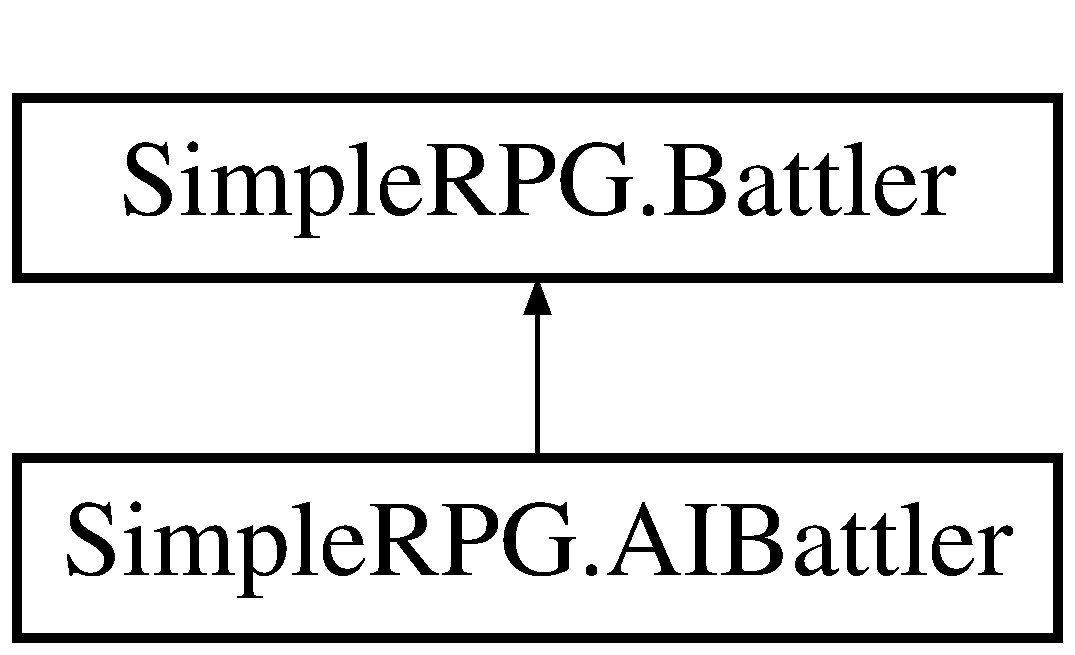
\includegraphics[height=2.000000cm]{class_simple_r_p_g_1_1_a_i_battler}
\end{center}
\end{figure}
\subsection*{Public Member Functions}
\begin{DoxyCompactItemize}
\item 
\hypertarget{class_simple_r_p_g_1_1_a_i_battler_a5343b886da17cdffff98bc39b56a4cf4}{{\bfseries A\-I\-Battler} (string req\-Name, int req\-Max\-H\-P, int req\-Max\-M\-P, int req\-Power, int req\-Will, int exp)}\label{class_simple_r_p_g_1_1_a_i_battler_a5343b886da17cdffff98bc39b56a4cf4}

\item 
\hypertarget{class_simple_r_p_g_1_1_a_i_battler_a3a1f2c68dda706c3a3f347e368275f3e}{override void {\bfseries take\-Turn} (\hyperlink{class_simple_r_p_g_1_1_states_1_1_battle_state}{Battle\-State} battle)}\label{class_simple_r_p_g_1_1_a_i_battler_a3a1f2c68dda706c3a3f347e368275f3e}

\item 
\hypertarget{class_simple_r_p_g_1_1_a_i_battler_a4938f4cfc972d4c6f923ba5e58bb0d9b}{override \hyperlink{class_simple_r_p_g_1_1_battler}{Battler} {\bfseries clone} ()}\label{class_simple_r_p_g_1_1_a_i_battler_a4938f4cfc972d4c6f923ba5e58bb0d9b}

\item 
int \hyperlink{class_simple_r_p_g_1_1_a_i_battler_a803b1a057e75f5a3d3c7c60b8147b6c7}{get\-Exp\-Earned} ()
\begin{DoxyCompactList}\small\item\em Gets the amount of E\-X\-P an \hyperlink{class_simple_r_p_g_1_1_a_i_battler}{A\-I\-Battler} is worth \end{DoxyCompactList}\end{DoxyCompactItemize}
\subsection*{Protected Attributes}
\begin{DoxyCompactItemize}
\item 
int \hyperlink{class_simple_r_p_g_1_1_a_i_battler_a3ccabe122a27e87289f6a40ca4da3c5d}{exp\-Earned}
\begin{DoxyCompactList}\small\item\em The amount of E\-X\-P a player earns for killing this battler \end{DoxyCompactList}\end{DoxyCompactItemize}
\subsection*{Additional Inherited Members}


\subsection{Member Function Documentation}
\hypertarget{class_simple_r_p_g_1_1_a_i_battler_a803b1a057e75f5a3d3c7c60b8147b6c7}{\index{Simple\-R\-P\-G\-::\-A\-I\-Battler@{Simple\-R\-P\-G\-::\-A\-I\-Battler}!get\-Exp\-Earned@{get\-Exp\-Earned}}
\index{get\-Exp\-Earned@{get\-Exp\-Earned}!SimpleRPG::AIBattler@{Simple\-R\-P\-G\-::\-A\-I\-Battler}}
\subsubsection[{get\-Exp\-Earned}]{\setlength{\rightskip}{0pt plus 5cm}int Simple\-R\-P\-G.\-A\-I\-Battler.\-get\-Exp\-Earned (
\begin{DoxyParamCaption}
{}
\end{DoxyParamCaption}
)\hspace{0.3cm}{\ttfamily [inline]}}}\label{class_simple_r_p_g_1_1_a_i_battler_a803b1a057e75f5a3d3c7c60b8147b6c7}


Gets the amount of E\-X\-P an \hyperlink{class_simple_r_p_g_1_1_a_i_battler}{A\-I\-Battler} is worth 

\begin{DoxyReturn}{Returns}
The E\-X\-P awarded for killing this battler
\end{DoxyReturn}


\subsection{Member Data Documentation}
\hypertarget{class_simple_r_p_g_1_1_a_i_battler_a3ccabe122a27e87289f6a40ca4da3c5d}{\index{Simple\-R\-P\-G\-::\-A\-I\-Battler@{Simple\-R\-P\-G\-::\-A\-I\-Battler}!exp\-Earned@{exp\-Earned}}
\index{exp\-Earned@{exp\-Earned}!SimpleRPG::AIBattler@{Simple\-R\-P\-G\-::\-A\-I\-Battler}}
\subsubsection[{exp\-Earned}]{\setlength{\rightskip}{0pt plus 5cm}int Simple\-R\-P\-G.\-A\-I\-Battler.\-exp\-Earned\hspace{0.3cm}{\ttfamily [protected]}}}\label{class_simple_r_p_g_1_1_a_i_battler_a3ccabe122a27e87289f6a40ca4da3c5d}


The amount of E\-X\-P a player earns for killing this battler 



The documentation for this class was generated from the following file\-:\begin{DoxyCompactItemize}
\item 
Simple\-R\-P\-G/\-Simple\-R\-P\-G/A\-I\-Battler.\-cs\end{DoxyCompactItemize}

\hypertarget{class_simple_r_p_g_1_1_animation}{\section{Simple\+R\+P\+G.\+Animation Class Reference}
\label{class_simple_r_p_g_1_1_animation}\index{Simple\+R\+P\+G.\+Animation@{Simple\+R\+P\+G.\+Animation}}
}
\subsection*{Static Public Member Functions}
\begin{DoxyCompactItemize}
\item 
\hypertarget{class_simple_r_p_g_1_1_animation_a6c30d271e7914db827c587792d36c1ce}{static void {\bfseries fade\+In} (\hyperlink{class_simple_r_p_g_1_1_drawable}{Drawable} drawable)}\label{class_simple_r_p_g_1_1_animation_a6c30d271e7914db827c587792d36c1ce}

\item 
\hypertarget{class_simple_r_p_g_1_1_animation_a8a5a03c9d244c3248c828f5c8c961f9f}{static void {\bfseries fade\+In} (\hyperlink{class_simple_r_p_g_1_1_drawable}{Drawable} drawable, int frames)}\label{class_simple_r_p_g_1_1_animation_a8a5a03c9d244c3248c828f5c8c961f9f}

\item 
\hypertarget{class_simple_r_p_g_1_1_animation_a289c9da41575652f1b2573722af62527}{static void {\bfseries fade\+Out} (\hyperlink{class_simple_r_p_g_1_1_drawable}{Drawable} drawable)}\label{class_simple_r_p_g_1_1_animation_a289c9da41575652f1b2573722af62527}

\item 
\hypertarget{class_simple_r_p_g_1_1_animation_a464fa54ff15747341f46bffa81e5a977}{static void {\bfseries fade\+Out} (\hyperlink{class_simple_r_p_g_1_1_drawable}{Drawable} drawable, int frames)}\label{class_simple_r_p_g_1_1_animation_a464fa54ff15747341f46bffa81e5a977}

\item 
\hypertarget{class_simple_r_p_g_1_1_animation_a70728603a4b9154a487cbb8eb8bbef04}{static void {\bfseries none\+In} (\hyperlink{class_simple_r_p_g_1_1_drawable}{Drawable} drawable)}\label{class_simple_r_p_g_1_1_animation_a70728603a4b9154a487cbb8eb8bbef04}

\item 
\hypertarget{class_simple_r_p_g_1_1_animation_aece2c00c52312d164c9ecf73f6f342d7}{static void {\bfseries none\+Out} (\hyperlink{class_simple_r_p_g_1_1_drawable}{Drawable} drawable)}\label{class_simple_r_p_g_1_1_animation_aece2c00c52312d164c9ecf73f6f342d7}

\item 
\hypertarget{class_simple_r_p_g_1_1_animation_a57887aeb5e46066b4426e2fa8d715175}{static void {\bfseries animate\+In} (\hyperlink{class_simple_r_p_g_1_1_drawable}{Drawable} drawable, Animation\+Type animation)}\label{class_simple_r_p_g_1_1_animation_a57887aeb5e46066b4426e2fa8d715175}

\item 
\hypertarget{class_simple_r_p_g_1_1_animation_a45e21ce9caf65cc315313632a1ecb201}{static void {\bfseries animate\+In} (\hyperlink{class_simple_r_p_g_1_1_drawable}{Drawable} drawable, Animation\+Type animation, int frames)}\label{class_simple_r_p_g_1_1_animation_a45e21ce9caf65cc315313632a1ecb201}

\item 
\hypertarget{class_simple_r_p_g_1_1_animation_a3fa90da4edd15c14c9a84ade2274dba0}{static void {\bfseries animate\+Out} (\hyperlink{class_simple_r_p_g_1_1_drawable}{Drawable} drawable, Animation\+Type animation)}\label{class_simple_r_p_g_1_1_animation_a3fa90da4edd15c14c9a84ade2274dba0}

\item 
\hypertarget{class_simple_r_p_g_1_1_animation_a7b584db5a90bc132011bb3f630193d4d}{static void {\bfseries animate\+Out} (\hyperlink{class_simple_r_p_g_1_1_drawable}{Drawable} drawable, Animation\+Type animation, int frames)}\label{class_simple_r_p_g_1_1_animation_a7b584db5a90bc132011bb3f630193d4d}

\end{DoxyCompactItemize}


The documentation for this class was generated from the following file\+:\begin{DoxyCompactItemize}
\item 
D\+:/\+Dropbox/\+Simple\+R\+P\+G/\+Simple\+R\+P\+G/\+Simple\+R\+P\+G/Animation.\+cs\end{DoxyCompactItemize}

\hypertarget{class_simple_r_p_g_1_1_states_1_1_battle_action_select_state}{\section{Simple\+R\+P\+G.\+States.\+Battle\+Action\+Select\+State Class Reference}
\label{class_simple_r_p_g_1_1_states_1_1_battle_action_select_state}\index{Simple\+R\+P\+G.\+States.\+Battle\+Action\+Select\+State@{Simple\+R\+P\+G.\+States.\+Battle\+Action\+Select\+State}}
}
Inheritance diagram for Simple\+R\+P\+G.\+States.\+Battle\+Action\+Select\+State\+:\begin{figure}[H]
\begin{center}
\leavevmode
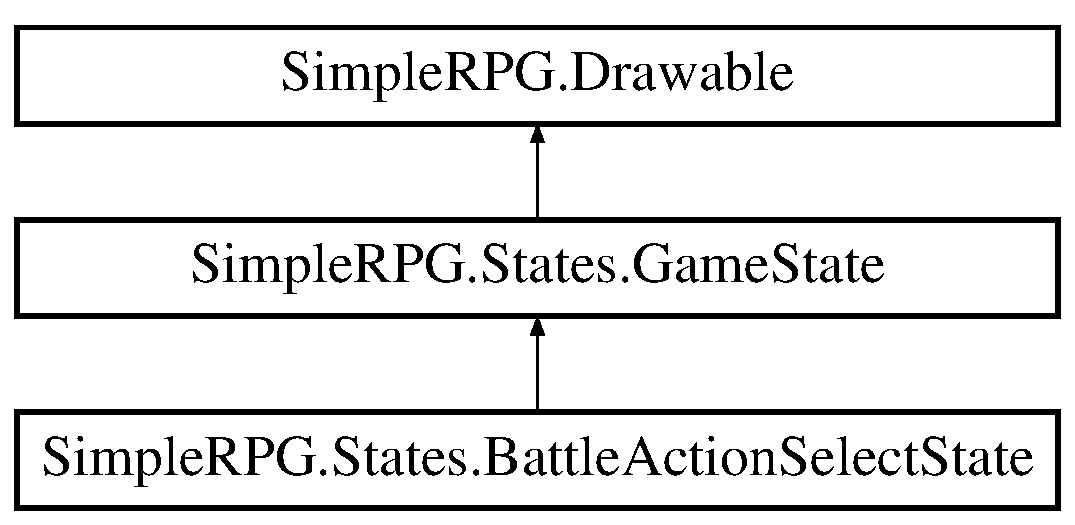
\includegraphics[height=3.000000cm]{class_simple_r_p_g_1_1_states_1_1_battle_action_select_state}
\end{center}
\end{figure}
\subsection*{Public Member Functions}
\begin{DoxyCompactItemize}
\item 
\hypertarget{class_simple_r_p_g_1_1_states_1_1_battle_action_select_state_aaa0f9b76c6f824efd3683ce6dccdcde6}{{\bfseries Battle\+Action\+Select\+State} (\hyperlink{class_simple_r_p_g_1_1_game1}{Game1} game, \hyperlink{class_simple_r_p_g_1_1_states_1_1_game_state}{Game\+State} parent, \hyperlink{class_simple_r_p_g_1_1_states_1_1_state_manager}{State\+Manager} manager, \hyperlink{class_simple_r_p_g_1_1_states_1_1_battle_state}{Battle\+State} battle)}\label{class_simple_r_p_g_1_1_states_1_1_battle_action_select_state_aaa0f9b76c6f824efd3683ce6dccdcde6}

\item 
\hypertarget{class_simple_r_p_g_1_1_states_1_1_battle_action_select_state_a1c5d4bbcde130994d834b345cdf1210a}{override void {\bfseries update} ()}\label{class_simple_r_p_g_1_1_states_1_1_battle_action_select_state_a1c5d4bbcde130994d834b345cdf1210a}

\item 
\hypertarget{class_simple_r_p_g_1_1_states_1_1_battle_action_select_state_a4e73b93f17d6be64765870b3b50987d6}{override void {\bfseries draw} (Sprite\+Batch sprite\+Batch)}\label{class_simple_r_p_g_1_1_states_1_1_battle_action_select_state_a4e73b93f17d6be64765870b3b50987d6}

\end{DoxyCompactItemize}
\subsection*{Protected Member Functions}
\begin{DoxyCompactItemize}
\item 
\hypertarget{class_simple_r_p_g_1_1_states_1_1_battle_action_select_state_ad1eaf46bf46fedfd8d465e9ad29b0018}{override void {\bfseries pass\+Data} (\hyperlink{class_simple_r_p_g_1_1_states_1_1_game_state}{Game\+State} sender, object data)}\label{class_simple_r_p_g_1_1_states_1_1_battle_action_select_state_ad1eaf46bf46fedfd8d465e9ad29b0018}

\end{DoxyCompactItemize}
\subsection*{Protected Attributes}
\begin{DoxyCompactItemize}
\item 
\hypertarget{class_simple_r_p_g_1_1_states_1_1_battle_action_select_state_a39f78e7281767700dfcd8725e0e0febe}{\hyperlink{class_simple_r_p_g_1_1_windows_1_1_list_box}{List\+Box} {\bfseries actions\+Window}}\label{class_simple_r_p_g_1_1_states_1_1_battle_action_select_state_a39f78e7281767700dfcd8725e0e0febe}

\item 
\hypertarget{class_simple_r_p_g_1_1_states_1_1_battle_action_select_state_ae1643c22fb4bbd4d594079fe83dabc60}{\hyperlink{class_simple_r_p_g_1_1_states_1_1_battle_state}{Battle\+State} {\bfseries battle\+State}}\label{class_simple_r_p_g_1_1_states_1_1_battle_action_select_state_ae1643c22fb4bbd4d594079fe83dabc60}

\end{DoxyCompactItemize}


The documentation for this class was generated from the following file\+:\begin{DoxyCompactItemize}
\item 
D\+:/\+Dropbox/\+Simple\+R\+P\+G/\+Simple\+R\+P\+G/\+Simple\+R\+P\+G/\+States/Battle\+Action\+Select\+State.\+cs\end{DoxyCompactItemize}

\hypertarget{class_simple_r_p_g_1_1_battler}{\section{Simple\-R\-P\-G.\-Battler Class Reference}
\label{class_simple_r_p_g_1_1_battler}\index{Simple\-R\-P\-G.\-Battler@{Simple\-R\-P\-G.\-Battler}}
}
Inheritance diagram for Simple\-R\-P\-G.\-Battler\-:\begin{figure}[H]
\begin{center}
\leavevmode
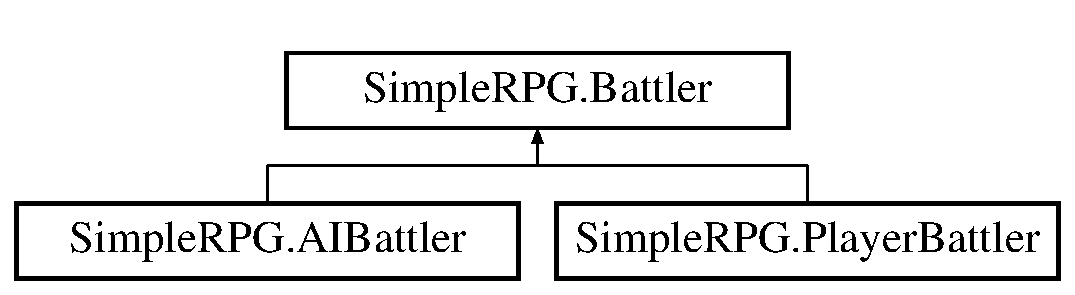
\includegraphics[height=2.000000cm]{class_simple_r_p_g_1_1_battler}
\end{center}
\end{figure}
\subsection*{Public Member Functions}
\begin{DoxyCompactItemize}
\item 
\hypertarget{class_simple_r_p_g_1_1_battler_a2d569c96856b4016469898c763cd80cd}{{\bfseries Battler} (string req\-Name, int req\-Max\-H\-P, int req\-Max\-M\-P, int req\-Power, int req\-Will)}\label{class_simple_r_p_g_1_1_battler_a2d569c96856b4016469898c763cd80cd}

\item 
\hypertarget{class_simple_r_p_g_1_1_battler_a33717e4b3db920bc7b1e91cd5923d440}{int {\bfseries get\-H\-P} ()}\label{class_simple_r_p_g_1_1_battler_a33717e4b3db920bc7b1e91cd5923d440}

\item 
\hypertarget{class_simple_r_p_g_1_1_battler_a4cfa0cad3cbcd37a0b778371f1bca4ac}{int {\bfseries get\-Max\-H\-P} ()}\label{class_simple_r_p_g_1_1_battler_a4cfa0cad3cbcd37a0b778371f1bca4ac}

\item 
\hypertarget{class_simple_r_p_g_1_1_battler_a545f4fc14281ea68bcbc096d74283027}{int {\bfseries get\-M\-P} ()}\label{class_simple_r_p_g_1_1_battler_a545f4fc14281ea68bcbc096d74283027}

\item 
\hypertarget{class_simple_r_p_g_1_1_battler_ac5abba3a65530d57317ffb745904ece5}{int {\bfseries get\-Max\-M\-P} ()}\label{class_simple_r_p_g_1_1_battler_ac5abba3a65530d57317ffb745904ece5}

\item 
\hypertarget{class_simple_r_p_g_1_1_battler_a26be8c08a8909d19e617ef6bc9d0751a}{int {\bfseries get\-Power} ()}\label{class_simple_r_p_g_1_1_battler_a26be8c08a8909d19e617ef6bc9d0751a}

\item 
\hypertarget{class_simple_r_p_g_1_1_battler_ab7539435d53520b9aaee35958e14472f}{int {\bfseries get\-Will} ()}\label{class_simple_r_p_g_1_1_battler_ab7539435d53520b9aaee35958e14472f}

\item 
\hypertarget{class_simple_r_p_g_1_1_battler_ad74e17513ba2f88b2bc6830ce9259e3b}{string {\bfseries get\-Name} ()}\label{class_simple_r_p_g_1_1_battler_ad74e17513ba2f88b2bc6830ce9259e3b}

\item 
\hypertarget{class_simple_r_p_g_1_1_battler_ae33a4b8a4af396dc2dfd26ad4938dcfa}{\hyperlink{class_simple_r_p_g_1_1_map_object}{Map\-Object} {\bfseries get\-Map\-Object} ()}\label{class_simple_r_p_g_1_1_battler_ae33a4b8a4af396dc2dfd26ad4938dcfa}

\item 
\hypertarget{class_simple_r_p_g_1_1_battler_a78193521e8fb0e7d60688c0a7bc303be}{bool {\bfseries is\-Alive} ()}\label{class_simple_r_p_g_1_1_battler_a78193521e8fb0e7d60688c0a7bc303be}

\item 
\hypertarget{class_simple_r_p_g_1_1_battler_a5a12026c4a85de2f20d568f183692f3e}{virtual int {\bfseries calculate\-Damage} ()}\label{class_simple_r_p_g_1_1_battler_a5a12026c4a85de2f20d568f183692f3e}

\item 
\hypertarget{class_simple_r_p_g_1_1_battler_abb9370052205c7cd49dd0865b83dadae}{virtual int {\bfseries defend} ()}\label{class_simple_r_p_g_1_1_battler_abb9370052205c7cd49dd0865b83dadae}

\item 
virtual void \hyperlink{class_simple_r_p_g_1_1_battler_a6afb1d99fc531bbbb9396e1205be1bed}{take\-Damage} (int damage)
\begin{DoxyCompactList}\small\item\em Causes a \hyperlink{class_simple_r_p_g_1_1_battler}{Battler} to directly lose a given amount of damage from their H\-P \end{DoxyCompactList}\item 
\hypertarget{class_simple_r_p_g_1_1_battler_aef46defbbb8c811f13c707099c3c8d4e}{virtual \hyperlink{class_simple_r_p_g_1_1_battler}{Battler} {\bfseries clone} ()}\label{class_simple_r_p_g_1_1_battler_aef46defbbb8c811f13c707099c3c8d4e}

\item 
\hypertarget{class_simple_r_p_g_1_1_battler_a92d63f259fbe5c79c7996db0744b8899}{virtual void {\bfseries take\-Turn} (\hyperlink{class_simple_r_p_g_1_1_states_1_1_battle_state}{Battle\-State} battle)}\label{class_simple_r_p_g_1_1_battler_a92d63f259fbe5c79c7996db0744b8899}

\item 
int \hyperlink{class_simple_r_p_g_1_1_battler_af3564d8cec0c5ca76601bf96e029df37}{physical\-Attack} (\hyperlink{class_simple_r_p_g_1_1_battler}{Battler} other)
\begin{DoxyCompactList}\small\item\em Causes this battler to physically attack a given other battler \end{DoxyCompactList}\item 
\hypertarget{class_simple_r_p_g_1_1_battler_a16434bead1bd62952eb74abc1be34863}{void {\bfseries add\-H\-P} (int value)}\label{class_simple_r_p_g_1_1_battler_a16434bead1bd62952eb74abc1be34863}

\item 
\hypertarget{class_simple_r_p_g_1_1_battler_a6b8fcc1465942de295cf4d181f752048}{void {\bfseries add\-M\-P} (int value)}\label{class_simple_r_p_g_1_1_battler_a6b8fcc1465942de295cf4d181f752048}

\item 
\hypertarget{class_simple_r_p_g_1_1_battler_a2507e5abe2a5029b276df32ef9241278}{void {\bfseries set\-Map\-Object} (\hyperlink{class_simple_r_p_g_1_1_map_object}{Map\-Object} o)}\label{class_simple_r_p_g_1_1_battler_a2507e5abe2a5029b276df32ef9241278}

\end{DoxyCompactItemize}
\subsection*{Static Public Attributes}
\begin{DoxyCompactItemize}
\item 
\hypertarget{class_simple_r_p_g_1_1_battler_ac83c439f26bd3abe3dcaa24d231bbfdc}{static int {\bfseries D\-A\-M\-A\-G\-E\-\_\-\-S\-C\-A\-L\-I\-N\-G} = 1}\label{class_simple_r_p_g_1_1_battler_ac83c439f26bd3abe3dcaa24d231bbfdc}

\item 
\hypertarget{class_simple_r_p_g_1_1_battler_a65a28ffcf2263397e640d77784652df3}{static Random {\bfseries random} = new Random()}\label{class_simple_r_p_g_1_1_battler_a65a28ffcf2263397e640d77784652df3}

\end{DoxyCompactItemize}
\subsection*{Protected Member Functions}
\begin{DoxyCompactItemize}
\item 
\hypertarget{class_simple_r_p_g_1_1_battler_a57e2a41105489240317dce088fc37c0f}{virtual bool {\bfseries is\-Crit} ()}\label{class_simple_r_p_g_1_1_battler_a57e2a41105489240317dce088fc37c0f}

\end{DoxyCompactItemize}
\subsection*{Protected Attributes}
\begin{DoxyCompactItemize}
\item 
\hypertarget{class_simple_r_p_g_1_1_battler_a07c64ffcc5fa74966f73c390b4730cbf}{int {\bfseries hp}}\label{class_simple_r_p_g_1_1_battler_a07c64ffcc5fa74966f73c390b4730cbf}

\item 
\hypertarget{class_simple_r_p_g_1_1_battler_a7d365863a653e2e113e013da68a3c448}{int {\bfseries mp}}\label{class_simple_r_p_g_1_1_battler_a7d365863a653e2e113e013da68a3c448}

\item 
\hypertarget{class_simple_r_p_g_1_1_battler_ad58a5b26c1489837ee06e85ea9525695}{int {\bfseries power}}\label{class_simple_r_p_g_1_1_battler_ad58a5b26c1489837ee06e85ea9525695}

\item 
\hypertarget{class_simple_r_p_g_1_1_battler_a2e7e9847ed0a9db282e0369964692034}{string {\bfseries name}}\label{class_simple_r_p_g_1_1_battler_a2e7e9847ed0a9db282e0369964692034}

\item 
\hypertarget{class_simple_r_p_g_1_1_battler_ae7435ffd77d4173ab28fec88591edf27}{\hyperlink{class_simple_r_p_g_1_1_map_object}{Map\-Object} {\bfseries map\-Object} = null}\label{class_simple_r_p_g_1_1_battler_ae7435ffd77d4173ab28fec88591edf27}

\end{DoxyCompactItemize}


\subsection{Member Function Documentation}
\hypertarget{class_simple_r_p_g_1_1_battler_af3564d8cec0c5ca76601bf96e029df37}{\index{Simple\-R\-P\-G\-::\-Battler@{Simple\-R\-P\-G\-::\-Battler}!physical\-Attack@{physical\-Attack}}
\index{physical\-Attack@{physical\-Attack}!SimpleRPG::Battler@{Simple\-R\-P\-G\-::\-Battler}}
\subsubsection[{physical\-Attack}]{\setlength{\rightskip}{0pt plus 5cm}int Simple\-R\-P\-G.\-Battler.\-physical\-Attack (
\begin{DoxyParamCaption}
\item[{{\bf Battler}}]{other}
\end{DoxyParamCaption}
)\hspace{0.3cm}{\ttfamily [inline]}}}\label{class_simple_r_p_g_1_1_battler_af3564d8cec0c5ca76601bf96e029df37}


Causes this battler to physically attack a given other battler 


\begin{DoxyParams}{Parameters}
{\em other} & The target battler that this battler will attack\\
\hline
\end{DoxyParams}
\begin{DoxyReturn}{Returns}
The amount of damage the target actually suffered
\end{DoxyReturn}
\hypertarget{class_simple_r_p_g_1_1_battler_a6afb1d99fc531bbbb9396e1205be1bed}{\index{Simple\-R\-P\-G\-::\-Battler@{Simple\-R\-P\-G\-::\-Battler}!take\-Damage@{take\-Damage}}
\index{take\-Damage@{take\-Damage}!SimpleRPG::Battler@{Simple\-R\-P\-G\-::\-Battler}}
\subsubsection[{take\-Damage}]{\setlength{\rightskip}{0pt plus 5cm}virtual void Simple\-R\-P\-G.\-Battler.\-take\-Damage (
\begin{DoxyParamCaption}
\item[{int}]{damage}
\end{DoxyParamCaption}
)\hspace{0.3cm}{\ttfamily [inline]}, {\ttfamily [virtual]}}}\label{class_simple_r_p_g_1_1_battler_a6afb1d99fc531bbbb9396e1205be1bed}


Causes a \hyperlink{class_simple_r_p_g_1_1_battler}{Battler} to directly lose a given amount of damage from their H\-P 


\begin{DoxyParams}{Parameters}
{\em damage} & Amount to subtract from the \hyperlink{class_simple_r_p_g_1_1_battler}{Battler}'s current H\-P\\
\hline
\end{DoxyParams}


The documentation for this class was generated from the following file\-:\begin{DoxyCompactItemize}
\item 
Simple\-R\-P\-G/\-Simple\-R\-P\-G/Battler.\-cs\end{DoxyCompactItemize}

\hypertarget{class_simple_r_p_g_1_1_states_1_1_battle_state}{\section{Simple\-R\-P\-G.\-States.\-Battle\-State Class Reference}
\label{class_simple_r_p_g_1_1_states_1_1_battle_state}\index{Simple\-R\-P\-G.\-States.\-Battle\-State@{Simple\-R\-P\-G.\-States.\-Battle\-State}}
}
Inheritance diagram for Simple\-R\-P\-G.\-States.\-Battle\-State\-:\begin{figure}[H]
\begin{center}
\leavevmode
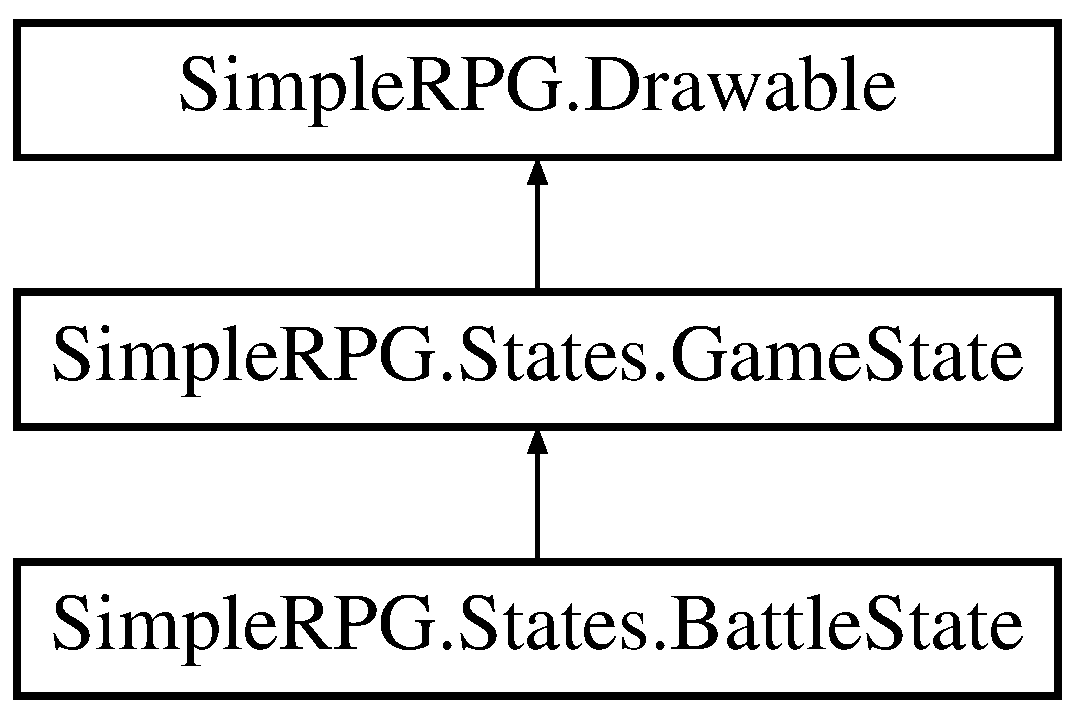
\includegraphics[height=3.000000cm]{class_simple_r_p_g_1_1_states_1_1_battle_state}
\end{center}
\end{figure}
\subsection*{Public Member Functions}
\begin{DoxyCompactItemize}
\item 
\hypertarget{class_simple_r_p_g_1_1_states_1_1_battle_state_a6f6ee41b383c1e50137ad9e3fbbdfcbe}{{\bfseries Battle\-State} (\hyperlink{class_simple_r_p_g_1_1_game1}{Game1} game, \hyperlink{class_simple_r_p_g_1_1_states_1_1_game_state}{Game\-State} parent, \hyperlink{class_simple_r_p_g_1_1_states_1_1_state_manager}{State\-Manager} manager)}\label{class_simple_r_p_g_1_1_states_1_1_battle_state_a6f6ee41b383c1e50137ad9e3fbbdfcbe}

\item 
\hypertarget{class_simple_r_p_g_1_1_states_1_1_battle_state_aea4acbb5ef3605fa73f59840d3f64d85}{override void {\bfseries draw} (Sprite\-Batch sprite\-Batch)}\label{class_simple_r_p_g_1_1_states_1_1_battle_state_aea4acbb5ef3605fa73f59840d3f64d85}

\item 
\hypertarget{class_simple_r_p_g_1_1_states_1_1_battle_state_ab34b5df3fa137fb63111568eb9fd6382}{override void {\bfseries update} ()}\label{class_simple_r_p_g_1_1_states_1_1_battle_state_ab34b5df3fa137fb63111568eb9fd6382}

\item 
\hypertarget{class_simple_r_p_g_1_1_states_1_1_battle_state_a71de4d97035523217f827c4dbbedb36e}{\hyperlink{class_simple_r_p_g_1_1_states_1_1_state_manager}{State\-Manager} {\bfseries get\-State\-Manager} ()}\label{class_simple_r_p_g_1_1_states_1_1_battle_state_a71de4d97035523217f827c4dbbedb36e}

\item 
\hypertarget{class_simple_r_p_g_1_1_states_1_1_battle_state_a219ad99cffee902574176cb9e88b0831}{\hyperlink{class_simple_r_p_g_1_1_game1}{Game1} {\bfseries get\-Game\-Ref} ()}\label{class_simple_r_p_g_1_1_states_1_1_battle_state_a219ad99cffee902574176cb9e88b0831}

\item 
List$<$ \hyperlink{class_simple_r_p_g_1_1_battler}{Battler} $>$ \hyperlink{class_simple_r_p_g_1_1_states_1_1_battle_state_a82c6a6de5de52d9586364607bb61d777}{get\-Enemies} (\hyperlink{class_simple_r_p_g_1_1_battler}{Battler} battler)
\begin{DoxyCompactList}\small\item\em Gets the enemies of a specific battler \end{DoxyCompactList}\item 
List$<$ \hyperlink{class_simple_r_p_g_1_1_battler}{Battler} $>$ \hyperlink{class_simple_r_p_g_1_1_states_1_1_battle_state_aafaee022fae4144c8606e7843db584fd}{get\-Enemies} ()
\begin{DoxyCompactList}\small\item\em Gets the enemies of the current battler \end{DoxyCompactList}\item 
\hypertarget{class_simple_r_p_g_1_1_states_1_1_battle_state_afea1b2b46a818c024abe7420daae1892}{\hyperlink{class_simple_r_p_g_1_1_battler}{Battler} {\bfseries get\-Current\-Battler} ()}\label{class_simple_r_p_g_1_1_states_1_1_battle_state_afea1b2b46a818c024abe7420daae1892}

\item 
\hypertarget{class_simple_r_p_g_1_1_states_1_1_battle_state_ab17e426b7d18e47c0f7f9bef8fc088dd}{void {\bfseries show\-Combat\-Result} (string result)}\label{class_simple_r_p_g_1_1_states_1_1_battle_state_ab17e426b7d18e47c0f7f9bef8fc088dd}

\item 
\hypertarget{class_simple_r_p_g_1_1_states_1_1_battle_state_ad4033eabfbc07f553de8888c4446a62f}{void {\bfseries show\-Combat\-Result} (\hyperlink{class_simple_r_p_g_1_1_battler}{Battler} attacker, \hyperlink{class_simple_r_p_g_1_1_battler}{Battler} defender, int damage)}\label{class_simple_r_p_g_1_1_states_1_1_battle_state_ad4033eabfbc07f553de8888c4446a62f}

\item 
\hypertarget{class_simple_r_p_g_1_1_states_1_1_battle_state_a30b8731548b6653aa0305bc7d7a2ee0b}{void {\bfseries show\-Combat\-Result} (\hyperlink{class_simple_r_p_g_1_1_combat_result}{Combat\-Result} result)}\label{class_simple_r_p_g_1_1_states_1_1_battle_state_a30b8731548b6653aa0305bc7d7a2ee0b}

\item 
\hypertarget{class_simple_r_p_g_1_1_states_1_1_battle_state_a94b60260339a45a2340e4c83d4ddcb0e}{List$<$ \hyperlink{class_simple_r_p_g_1_1_battler}{Battler} $>$ {\bfseries get\-All\-Combatants} ()}\label{class_simple_r_p_g_1_1_states_1_1_battle_state_a94b60260339a45a2340e4c83d4ddcb0e}

\item 
\hypertarget{class_simple_r_p_g_1_1_states_1_1_battle_state_a90dd9cf46e142b4136b8b7e8707228bf}{int {\bfseries get\-Total\-Exp} ()}\label{class_simple_r_p_g_1_1_states_1_1_battle_state_a90dd9cf46e142b4136b8b7e8707228bf}

\item 
\hypertarget{class_simple_r_p_g_1_1_states_1_1_battle_state_a37be2a882cc9772ddcf91f11ece6a83a}{override void {\bfseries exit} ()}\label{class_simple_r_p_g_1_1_states_1_1_battle_state_a37be2a882cc9772ddcf91f11ece6a83a}

\end{DoxyCompactItemize}
\subsection*{Protected Member Functions}
\begin{DoxyCompactItemize}
\item 
virtual bool \hyperlink{class_simple_r_p_g_1_1_states_1_1_battle_state_a5075306cb94df8b52bfabf2bb4971dba}{check\-Battle\-End} ()
\begin{DoxyCompactList}\small\item\em Checks if the enemy party has any living members, and that there are no messages on screen \end{DoxyCompactList}\item 
\hypertarget{class_simple_r_p_g_1_1_states_1_1_battle_state_a66068004749422203c514634de5c95a6}{void {\bfseries next\-Turn} ()}\label{class_simple_r_p_g_1_1_states_1_1_battle_state_a66068004749422203c514634de5c95a6}

\end{DoxyCompactItemize}
\subsection*{Protected Attributes}
\begin{DoxyCompactItemize}
\item 
\hypertarget{class_simple_r_p_g_1_1_states_1_1_battle_state_a8ee2e240ea8fef49273421e887c2a5b1}{List$<$ \hyperlink{class_simple_r_p_g_1_1_battler}{Battler} $>$ {\bfseries player\-Party}}\label{class_simple_r_p_g_1_1_states_1_1_battle_state_a8ee2e240ea8fef49273421e887c2a5b1}

\item 
\hypertarget{class_simple_r_p_g_1_1_states_1_1_battle_state_af412109d775d28d6fc0644d033880424}{List$<$ \hyperlink{class_simple_r_p_g_1_1_a_i_battler}{A\-I\-Battler} $>$ {\bfseries enemy\-Party}}\label{class_simple_r_p_g_1_1_states_1_1_battle_state_af412109d775d28d6fc0644d033880424}

\item 
\hypertarget{class_simple_r_p_g_1_1_states_1_1_battle_state_a0810fb7d1b97d2e8f18f02e4ec90708e}{\hyperlink{class_simple_r_p_g_1_1_battler}{Battler} {\bfseries current\-Battler}}\label{class_simple_r_p_g_1_1_states_1_1_battle_state_a0810fb7d1b97d2e8f18f02e4ec90708e}

\item 
\hypertarget{class_simple_r_p_g_1_1_states_1_1_battle_state_a322abc88cfc8f9911b39ba2d0954189b}{Queue$<$ \hyperlink{class_simple_r_p_g_1_1_battler}{Battler} $>$ {\bfseries battle\-Queue}}\label{class_simple_r_p_g_1_1_states_1_1_battle_state_a322abc88cfc8f9911b39ba2d0954189b}

\item 
\hypertarget{class_simple_r_p_g_1_1_states_1_1_battle_state_a2220bb7da4a4a23bb41b7affb6bf045c}{\hyperlink{class_simple_r_p_g_1_1_states_1_1_state_manager}{State\-Manager} {\bfseries battle\-State\-Manager}}\label{class_simple_r_p_g_1_1_states_1_1_battle_state_a2220bb7da4a4a23bb41b7affb6bf045c}

\item 
\hypertarget{class_simple_r_p_g_1_1_states_1_1_battle_state_a851189a4c36d8f38c2c36882b64c3d8b}{List$<$ \hyperlink{class_simple_r_p_g_1_1_windows_1_1_window}{Window} $>$ {\bfseries windows}}\label{class_simple_r_p_g_1_1_states_1_1_battle_state_a851189a4c36d8f38c2c36882b64c3d8b}

\item 
\hypertarget{class_simple_r_p_g_1_1_states_1_1_battle_state_a01ac843035cd5438964132ff543ce30f}{List$<$ \hyperlink{class_simple_r_p_g_1_1_widgets_1_1_text_widget}{Text\-Widget} $>$ {\bfseries widgets}}\label{class_simple_r_p_g_1_1_states_1_1_battle_state_a01ac843035cd5438964132ff543ce30f}

\item 
\hypertarget{class_simple_r_p_g_1_1_states_1_1_battle_state_a14b7f61ded8f59006ea6744db662c7da}{List$<$ \hyperlink{class_simple_r_p_g_1_1_map_object}{Map\-Object} $>$ {\bfseries added\-To\-Map}}\label{class_simple_r_p_g_1_1_states_1_1_battle_state_a14b7f61ded8f59006ea6744db662c7da}

\end{DoxyCompactItemize}


\subsection{Member Function Documentation}
\hypertarget{class_simple_r_p_g_1_1_states_1_1_battle_state_a5075306cb94df8b52bfabf2bb4971dba}{\index{Simple\-R\-P\-G\-::\-States\-::\-Battle\-State@{Simple\-R\-P\-G\-::\-States\-::\-Battle\-State}!check\-Battle\-End@{check\-Battle\-End}}
\index{check\-Battle\-End@{check\-Battle\-End}!SimpleRPG::States::BattleState@{Simple\-R\-P\-G\-::\-States\-::\-Battle\-State}}
\subsubsection[{check\-Battle\-End}]{\setlength{\rightskip}{0pt plus 5cm}virtual bool Simple\-R\-P\-G.\-States.\-Battle\-State.\-check\-Battle\-End (
\begin{DoxyParamCaption}
{}
\end{DoxyParamCaption}
)\hspace{0.3cm}{\ttfamily [inline]}, {\ttfamily [protected]}, {\ttfamily [virtual]}}}\label{class_simple_r_p_g_1_1_states_1_1_battle_state_a5075306cb94df8b52bfabf2bb4971dba}


Checks if the enemy party has any living members, and that there are no messages on screen 

\begin{DoxyReturn}{Returns}
Returns false if there are some living enemies, or true if the battle is done
\end{DoxyReturn}
\hypertarget{class_simple_r_p_g_1_1_states_1_1_battle_state_a82c6a6de5de52d9586364607bb61d777}{\index{Simple\-R\-P\-G\-::\-States\-::\-Battle\-State@{Simple\-R\-P\-G\-::\-States\-::\-Battle\-State}!get\-Enemies@{get\-Enemies}}
\index{get\-Enemies@{get\-Enemies}!SimpleRPG::States::BattleState@{Simple\-R\-P\-G\-::\-States\-::\-Battle\-State}}
\subsubsection[{get\-Enemies}]{\setlength{\rightskip}{0pt plus 5cm}List$<${\bf Battler}$>$ Simple\-R\-P\-G.\-States.\-Battle\-State.\-get\-Enemies (
\begin{DoxyParamCaption}
\item[{{\bf Battler}}]{battler}
\end{DoxyParamCaption}
)\hspace{0.3cm}{\ttfamily [inline]}}}\label{class_simple_r_p_g_1_1_states_1_1_battle_state_a82c6a6de5de52d9586364607bb61d777}


Gets the enemies of a specific battler 


\begin{DoxyParams}{Parameters}
{\em battler} & The battler whose enemies are wanted\\
\hline
\end{DoxyParams}
\begin{DoxyReturn}{Returns}
The enemies of the specified battler
\end{DoxyReturn}
\hypertarget{class_simple_r_p_g_1_1_states_1_1_battle_state_aafaee022fae4144c8606e7843db584fd}{\index{Simple\-R\-P\-G\-::\-States\-::\-Battle\-State@{Simple\-R\-P\-G\-::\-States\-::\-Battle\-State}!get\-Enemies@{get\-Enemies}}
\index{get\-Enemies@{get\-Enemies}!SimpleRPG::States::BattleState@{Simple\-R\-P\-G\-::\-States\-::\-Battle\-State}}
\subsubsection[{get\-Enemies}]{\setlength{\rightskip}{0pt plus 5cm}List$<${\bf Battler}$>$ Simple\-R\-P\-G.\-States.\-Battle\-State.\-get\-Enemies (
\begin{DoxyParamCaption}
{}
\end{DoxyParamCaption}
)\hspace{0.3cm}{\ttfamily [inline]}}}\label{class_simple_r_p_g_1_1_states_1_1_battle_state_aafaee022fae4144c8606e7843db584fd}


Gets the enemies of the current battler 

\begin{DoxyReturn}{Returns}
The enemies of the current battler
\end{DoxyReturn}


The documentation for this class was generated from the following file\-:\begin{DoxyCompactItemize}
\item 
Simple\-R\-P\-G/\-Simple\-R\-P\-G/\-States/Battle\-State.\-cs\end{DoxyCompactItemize}

\hypertarget{class_simple_r_p_g_1_1_camera}{\section{Simple\+R\+P\+G.\+Camera Class Reference}
\label{class_simple_r_p_g_1_1_camera}\index{Simple\+R\+P\+G.\+Camera@{Simple\+R\+P\+G.\+Camera}}
}
Inheritance diagram for Simple\+R\+P\+G.\+Camera\+:\begin{figure}[H]
\begin{center}
\leavevmode
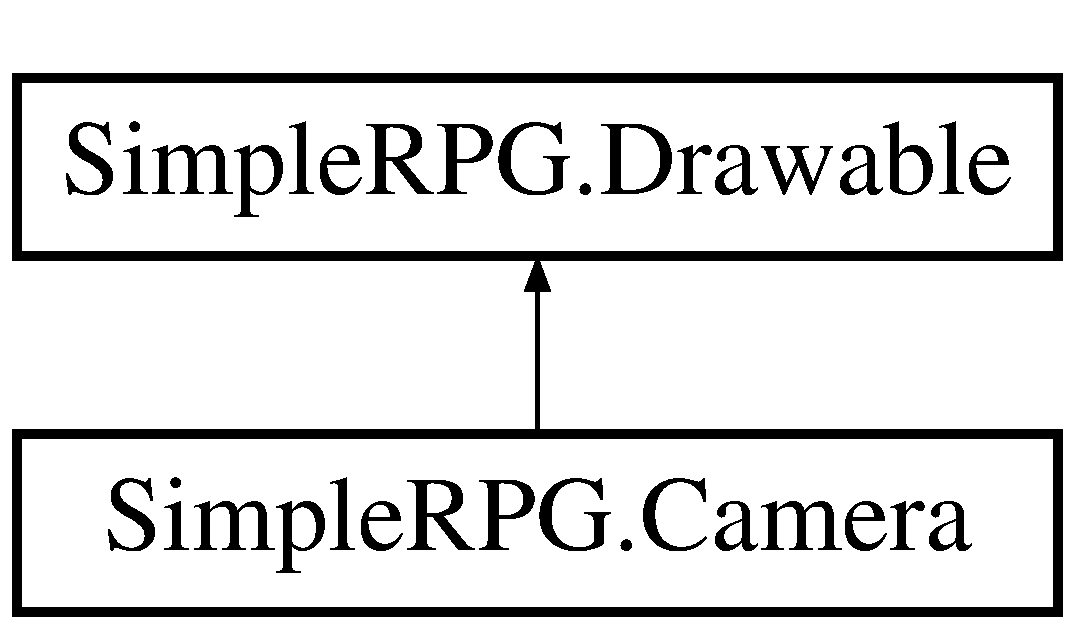
\includegraphics[height=2.000000cm]{class_simple_r_p_g_1_1_camera}
\end{center}
\end{figure}
\subsection*{Public Member Functions}
\begin{DoxyCompactItemize}
\item 
\hypertarget{class_simple_r_p_g_1_1_camera_a3df3d47b11911673673c2b6f4ca93f2b}{{\bfseries Camera} (int req\+Width, int req\+Height)}\label{class_simple_r_p_g_1_1_camera_a3df3d47b11911673673c2b6f4ca93f2b}

\item 
\hypertarget{class_simple_r_p_g_1_1_camera_a4aff6363c8bdfabb2f56fe779272ad0b}{void {\bfseries update} ()}\label{class_simple_r_p_g_1_1_camera_a4aff6363c8bdfabb2f56fe779272ad0b}

\item 
\hypertarget{class_simple_r_p_g_1_1_camera_a57ce092c1b4078fd61a3179c2ab8b93c}{void {\bfseries draw} (Sprite\+Batch sprite\+Batch)}\label{class_simple_r_p_g_1_1_camera_a57ce092c1b4078fd61a3179c2ab8b93c}

\item 
\hypertarget{class_simple_r_p_g_1_1_camera_aa79c2b9a8151f5441c694f5e6ccd2cfd}{void {\bfseries set\+Map} (\hyperlink{class_simple_r_p_g_1_1_tile_map}{Tile\+Map} new\+Map)}\label{class_simple_r_p_g_1_1_camera_aa79c2b9a8151f5441c694f5e6ccd2cfd}

\item 
\hypertarget{class_simple_r_p_g_1_1_camera_ac252db1ef72425c155d7914a408320bd}{void {\bfseries set\+Following} (\hyperlink{class_simple_r_p_g_1_1_map_object}{Map\+Object} to\+Follow)}\label{class_simple_r_p_g_1_1_camera_ac252db1ef72425c155d7914a408320bd}

\item 
\hypertarget{class_simple_r_p_g_1_1_camera_a0fd8e940f8f45fa9b2d6a8dc625211ea}{void {\bfseries follow} ()}\label{class_simple_r_p_g_1_1_camera_a0fd8e940f8f45fa9b2d6a8dc625211ea}

\item 
\hypertarget{class_simple_r_p_g_1_1_camera_a9765209fd53634d10039c02ac3efc58e}{void {\bfseries move} (Point value)}\label{class_simple_r_p_g_1_1_camera_a9765209fd53634d10039c02ac3efc58e}

\item 
\hypertarget{class_simple_r_p_g_1_1_camera_a49af7ca99f42cb5fe226fdc40c9cf4bd}{void {\bfseries increase\+Zoom} ()}\label{class_simple_r_p_g_1_1_camera_a49af7ca99f42cb5fe226fdc40c9cf4bd}

\item 
\hypertarget{class_simple_r_p_g_1_1_camera_a5a97dec2fa082efa5b3d58ac96d04af3}{void {\bfseries decrease\+Zoom} ()}\label{class_simple_r_p_g_1_1_camera_a5a97dec2fa082efa5b3d58ac96d04af3}

\item 
\hypertarget{class_simple_r_p_g_1_1_camera_a8822f4b9d972bd6c4cf21d0c1c74ee1f}{void {\bfseries set\+Zoom} (int value)}\label{class_simple_r_p_g_1_1_camera_a8822f4b9d972bd6c4cf21d0c1c74ee1f}

\end{DoxyCompactItemize}
\subsection*{Protected Attributes}
\begin{DoxyCompactItemize}
\item 
\hypertarget{class_simple_r_p_g_1_1_camera_ab0fea3d111b817fcb7f838b4648c4657}{int {\bfseries width}}\label{class_simple_r_p_g_1_1_camera_ab0fea3d111b817fcb7f838b4648c4657}

\item 
\hypertarget{class_simple_r_p_g_1_1_camera_ae1387580f2a0ebd55db53956c6dd13e5}{Point {\bfseries position}}\label{class_simple_r_p_g_1_1_camera_ae1387580f2a0ebd55db53956c6dd13e5}

\item 
\hypertarget{class_simple_r_p_g_1_1_camera_a1641f20a80724c541768c011ad2764dd}{\hyperlink{class_simple_r_p_g_1_1_tile_map}{Tile\+Map} {\bfseries map}}\label{class_simple_r_p_g_1_1_camera_a1641f20a80724c541768c011ad2764dd}

\item 
\hypertarget{class_simple_r_p_g_1_1_camera_aca69b516daceee441b7720ada3c332e4}{\hyperlink{class_simple_r_p_g_1_1_map_object}{Map\+Object} {\bfseries following}}\label{class_simple_r_p_g_1_1_camera_aca69b516daceee441b7720ada3c332e4}

\item 
\hypertarget{class_simple_r_p_g_1_1_camera_a107cbdb4e731179affca5292ea1b2a4a}{int {\bfseries scale} = 3}\label{class_simple_r_p_g_1_1_camera_a107cbdb4e731179affca5292ea1b2a4a}

\end{DoxyCompactItemize}


The documentation for this class was generated from the following file\+:\begin{DoxyCompactItemize}
\item 
D\+:/\+Dropbox/\+Simple\+R\+P\+G/\+Simple\+R\+P\+G/\+Simple\+R\+P\+G/Camera.\+cs\end{DoxyCompactItemize}

\hypertarget{class_simple_r_p_g_1_1_drawable}{\section{Simple\-R\-P\-G.\-Drawable Class Reference}
\label{class_simple_r_p_g_1_1_drawable}\index{Simple\-R\-P\-G.\-Drawable@{Simple\-R\-P\-G.\-Drawable}}
}
Inheritance diagram for Simple\-R\-P\-G.\-Drawable\-:\begin{figure}[H]
\begin{center}
\leavevmode
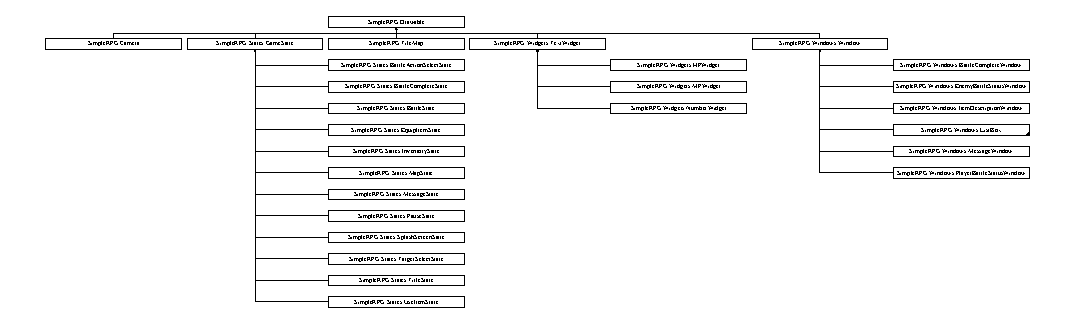
\includegraphics[height=3.902439cm]{class_simple_r_p_g_1_1_drawable}
\end{center}
\end{figure}
\subsection*{Public Member Functions}
\begin{DoxyCompactItemize}
\item 
\hypertarget{class_simple_r_p_g_1_1_drawable_a5a0bce0391462d1a6dd89f42b2db285d}{virtual void {\bfseries update} ()}\label{class_simple_r_p_g_1_1_drawable_a5a0bce0391462d1a6dd89f42b2db285d}

\item 
\hypertarget{class_simple_r_p_g_1_1_drawable_af8aa3c3839a2bba48eb04e314ebed6df}{virtual void {\bfseries draw} (Sprite\-Batch sprite\-Batch)}\label{class_simple_r_p_g_1_1_drawable_af8aa3c3839a2bba48eb04e314ebed6df}

\item 
\hypertarget{class_simple_r_p_g_1_1_drawable_a25a8469074c74391bce1d6cbf9e44c5d}{void {\bfseries set\-Opacity} (float value)}\label{class_simple_r_p_g_1_1_drawable_a25a8469074c74391bce1d6cbf9e44c5d}

\item 
\hypertarget{class_simple_r_p_g_1_1_drawable_a9210f178abf928fa27b822d73c7c0005}{void {\bfseries set\-Opacity} (float value, int frames\-To\-Fade)}\label{class_simple_r_p_g_1_1_drawable_a9210f178abf928fa27b822d73c7c0005}

\item 
\hypertarget{class_simple_r_p_g_1_1_drawable_a6c4159739e886073e9fc6567825c176e}{float {\bfseries get\-Opacity} ()}\label{class_simple_r_p_g_1_1_drawable_a6c4159739e886073e9fc6567825c176e}

\end{DoxyCompactItemize}
\subsection*{Protected Attributes}
\begin{DoxyCompactItemize}
\item 
\hypertarget{class_simple_r_p_g_1_1_drawable_a7378ddf59da70427cd4315925a9273b3}{float {\bfseries opacity} = 1}\label{class_simple_r_p_g_1_1_drawable_a7378ddf59da70427cd4315925a9273b3}

\end{DoxyCompactItemize}


The documentation for this class was generated from the following file\-:\begin{DoxyCompactItemize}
\item 
Simple\-R\-P\-G/\-Simple\-R\-P\-G/Drawable.\-cs\end{DoxyCompactItemize}

\hypertarget{class_simple_r_p_g_1_1_drawable_layer}{\section{Simple\+R\+P\+G.\+Drawable\+Layer Class Reference}
\label{class_simple_r_p_g_1_1_drawable_layer}\index{Simple\+R\+P\+G.\+Drawable\+Layer@{Simple\+R\+P\+G.\+Drawable\+Layer}}
}
Inheritance diagram for Simple\+R\+P\+G.\+Drawable\+Layer\+:\begin{figure}[H]
\begin{center}
\leavevmode
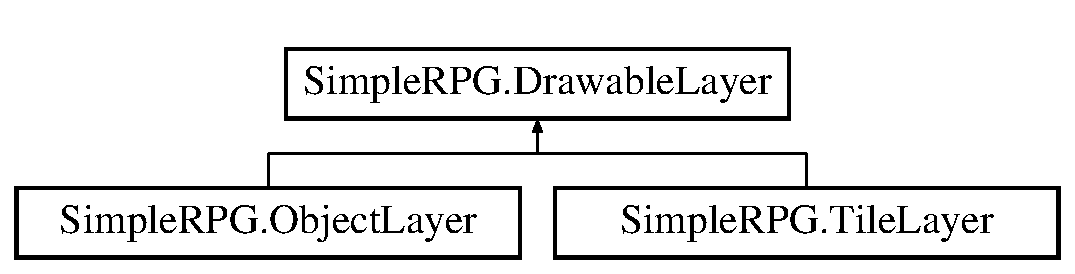
\includegraphics[height=2.000000cm]{class_simple_r_p_g_1_1_drawable_layer}
\end{center}
\end{figure}
\subsection*{Public Member Functions}
\begin{DoxyCompactItemize}
\item 
\hypertarget{class_simple_r_p_g_1_1_drawable_layer_a0803d17ddf796c736412a3ec9b099bea}{virtual void {\bfseries update} ()}\label{class_simple_r_p_g_1_1_drawable_layer_a0803d17ddf796c736412a3ec9b099bea}

\item 
\hypertarget{class_simple_r_p_g_1_1_drawable_layer_abf1e9fa363dd592d5c01935e46bcd71e}{virtual void {\bfseries draw} (Sprite\+Batch sprite\+Batch, Point first\+Tile, int tiles\+Across, int tiles\+Down, Point offset)}\label{class_simple_r_p_g_1_1_drawable_layer_abf1e9fa363dd592d5c01935e46bcd71e}

\item 
\hypertarget{class_simple_r_p_g_1_1_drawable_layer_af4129d9ebd2e139ccaf2618b0c93e1bb}{virtual void {\bfseries draw} (Sprite\+Batch sprite\+Batch, Point first\+Tile, int tiles\+Across, int tiles\+Down, Point offset, int scale)}\label{class_simple_r_p_g_1_1_drawable_layer_af4129d9ebd2e139ccaf2618b0c93e1bb}

\item 
\hypertarget{class_simple_r_p_g_1_1_drawable_layer_a87911cd99c0a4d379d0c3f1c2f0af84c}{void {\bfseries set\+Opacity} (float value)}\label{class_simple_r_p_g_1_1_drawable_layer_a87911cd99c0a4d379d0c3f1c2f0af84c}

\item 
\hypertarget{class_simple_r_p_g_1_1_drawable_layer_a2267e4b442be555ea7386e83295e832a}{void {\bfseries add\+Opacity} (float value)}\label{class_simple_r_p_g_1_1_drawable_layer_a2267e4b442be555ea7386e83295e832a}

\item 
\hypertarget{class_simple_r_p_g_1_1_drawable_layer_a8891ce4a9e4d5fbfa993cb6b0073dfbf}{float {\bfseries get\+Opacity} ()}\label{class_simple_r_p_g_1_1_drawable_layer_a8891ce4a9e4d5fbfa993cb6b0073dfbf}

\item 
\hypertarget{class_simple_r_p_g_1_1_drawable_layer_adb33676bd4d70ddec74667c74f4e0c0e}{virtual Passability {\bfseries get\+Passability} (int x, int y)}\label{class_simple_r_p_g_1_1_drawable_layer_adb33676bd4d70ddec74667c74f4e0c0e}

\end{DoxyCompactItemize}
\subsection*{Protected Member Functions}
\begin{DoxyCompactItemize}
\item 
\hypertarget{class_simple_r_p_g_1_1_drawable_layer_a015e72b02bc28151e2d42e6d22420c00}{{\bfseries Drawable\+Layer} (string req\+Name)}\label{class_simple_r_p_g_1_1_drawable_layer_a015e72b02bc28151e2d42e6d22420c00}

\end{DoxyCompactItemize}
\subsection*{Protected Attributes}
\begin{DoxyCompactItemize}
\item 
\hypertarget{class_simple_r_p_g_1_1_drawable_layer_a613c63f79a863ca37dbd1f18ea4c2915}{float {\bfseries opacity}}\label{class_simple_r_p_g_1_1_drawable_layer_a613c63f79a863ca37dbd1f18ea4c2915}

\item 
\hypertarget{class_simple_r_p_g_1_1_drawable_layer_ac006479228e4588dc3aef0d885c2cbfc}{string {\bfseries name}}\label{class_simple_r_p_g_1_1_drawable_layer_ac006479228e4588dc3aef0d885c2cbfc}

\end{DoxyCompactItemize}


The documentation for this class was generated from the following file\+:\begin{DoxyCompactItemize}
\item 
D\+:/\+Dropbox/\+Simple\+R\+P\+G/\+Simple\+R\+P\+G/\+Simple\+R\+P\+G/Drawable\+Layer.\+cs\end{DoxyCompactItemize}

\hypertarget{class_simple_r_p_g_1_1_enemy_manager}{\section{Simple\+R\+P\+G.\+Enemy\+Manager Class Reference}
\label{class_simple_r_p_g_1_1_enemy_manager}\index{Simple\+R\+P\+G.\+Enemy\+Manager@{Simple\+R\+P\+G.\+Enemy\+Manager}}
}
\subsection*{Static Public Member Functions}
\begin{DoxyCompactItemize}
\item 
\hypertarget{class_simple_r_p_g_1_1_enemy_manager_a14baa62389dfdead6dfcee80e5011e11}{static void {\bfseries add\+Enemy} (\hyperlink{class_simple_r_p_g_1_1_battler}{Battler} new\+Enemy)}\label{class_simple_r_p_g_1_1_enemy_manager_a14baa62389dfdead6dfcee80e5011e11}

\item 
\hypertarget{class_simple_r_p_g_1_1_enemy_manager_a06f546f669c154cc8365b2bbeaca5f4f}{static \hyperlink{class_simple_r_p_g_1_1_battler}{Battler} {\bfseries get\+Enemy} (string enemy\+Name)}\label{class_simple_r_p_g_1_1_enemy_manager_a06f546f669c154cc8365b2bbeaca5f4f}

\item 
\hypertarget{class_simple_r_p_g_1_1_enemy_manager_a398c5141a704ce9c65606465dca71700}{static void {\bfseries initialize} ()}\label{class_simple_r_p_g_1_1_enemy_manager_a398c5141a704ce9c65606465dca71700}

\end{DoxyCompactItemize}


The documentation for this class was generated from the following file\+:\begin{DoxyCompactItemize}
\item 
D\+:/\+Dropbox/\+Simple\+R\+P\+G/\+Simple\+R\+P\+G/\+Simple\+R\+P\+G/Enemy\+Manager.\+cs\end{DoxyCompactItemize}

\hypertarget{class_simple_r_p_g_1_1_events_1_1_event}{\section{Simple\+R\+P\+G.\+Events.\+Event Class Reference}
\label{class_simple_r_p_g_1_1_events_1_1_event}\index{Simple\+R\+P\+G.\+Events.\+Event@{Simple\+R\+P\+G.\+Events.\+Event}}
}
Inheritance diagram for Simple\+R\+P\+G.\+Events.\+Event\+:\begin{figure}[H]
\begin{center}
\leavevmode
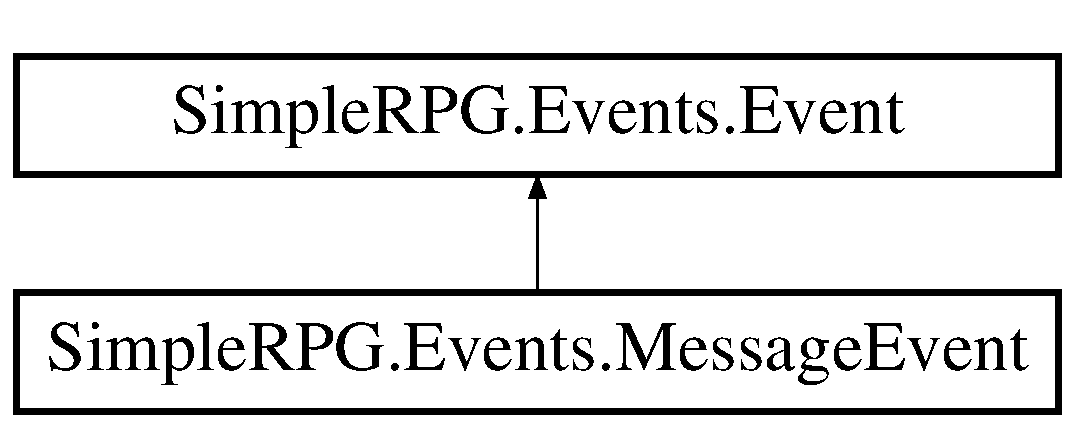
\includegraphics[height=2.000000cm]{class_simple_r_p_g_1_1_events_1_1_event}
\end{center}
\end{figure}
\subsection*{Public Member Functions}
\begin{DoxyCompactItemize}
\item 
\hypertarget{class_simple_r_p_g_1_1_events_1_1_event_ab7dfb6fbd4e0d5f9489bab5a7c129230}{{\bfseries Event} (\hyperlink{class_simple_r_p_g_1_1_game1}{Game1} game, \hyperlink{class_simple_r_p_g_1_1_states_1_1_state_manager}{State\+Manager} manager)}\label{class_simple_r_p_g_1_1_events_1_1_event_ab7dfb6fbd4e0d5f9489bab5a7c129230}

\item 
\hypertarget{class_simple_r_p_g_1_1_events_1_1_event_ad2ba4008dc240e6f5112def47a7239bd}{virtual void {\bfseries start} ()}\label{class_simple_r_p_g_1_1_events_1_1_event_ad2ba4008dc240e6f5112def47a7239bd}

\item 
\hypertarget{class_simple_r_p_g_1_1_events_1_1_event_af827a485fcc3cd3e52a3ecd306bf0c57}{virtual void {\bfseries update} ()}\label{class_simple_r_p_g_1_1_events_1_1_event_af827a485fcc3cd3e52a3ecd306bf0c57}

\item 
\hypertarget{class_simple_r_p_g_1_1_events_1_1_event_aaa5a7c0b6f04cd6564be3bcd69621279}{Boolean {\bfseries is\+Finished} ()}\label{class_simple_r_p_g_1_1_events_1_1_event_aaa5a7c0b6f04cd6564be3bcd69621279}

\end{DoxyCompactItemize}
\subsection*{Protected Attributes}
\begin{DoxyCompactItemize}
\item 
\hypertarget{class_simple_r_p_g_1_1_events_1_1_event_af9e2be9b16bc904e3276ed114a4d11a5}{Boolean {\bfseries finished} = false}\label{class_simple_r_p_g_1_1_events_1_1_event_af9e2be9b16bc904e3276ed114a4d11a5}

\item 
\hypertarget{class_simple_r_p_g_1_1_events_1_1_event_a60fe4373065c00d225e11f24c785197c}{\hyperlink{class_simple_r_p_g_1_1_game1}{Game1} {\bfseries game\+Ref}}\label{class_simple_r_p_g_1_1_events_1_1_event_a60fe4373065c00d225e11f24c785197c}

\item 
\hypertarget{class_simple_r_p_g_1_1_events_1_1_event_a08f23edd033e042324051522a1533c84}{\hyperlink{class_simple_r_p_g_1_1_states_1_1_state_manager}{State\+Manager} {\bfseries state\+Manager}}\label{class_simple_r_p_g_1_1_events_1_1_event_a08f23edd033e042324051522a1533c84}

\end{DoxyCompactItemize}


The documentation for this class was generated from the following file\+:\begin{DoxyCompactItemize}
\item 
D\+:/\+Dropbox/\+Simple\+R\+P\+G/\+Simple\+R\+P\+G/\+Simple\+R\+P\+G/\+Events/Event.\+cs\end{DoxyCompactItemize}

\hypertarget{class_simple_r_p_g_1_1_game1}{\section{Simple\-R\-P\-G.\-Game1 Class Reference}
\label{class_simple_r_p_g_1_1_game1}\index{Simple\-R\-P\-G.\-Game1@{Simple\-R\-P\-G.\-Game1}}
}


This is the main type for your game  


Inheritance diagram for Simple\-R\-P\-G.\-Game1\-:\begin{figure}[H]
\begin{center}
\leavevmode
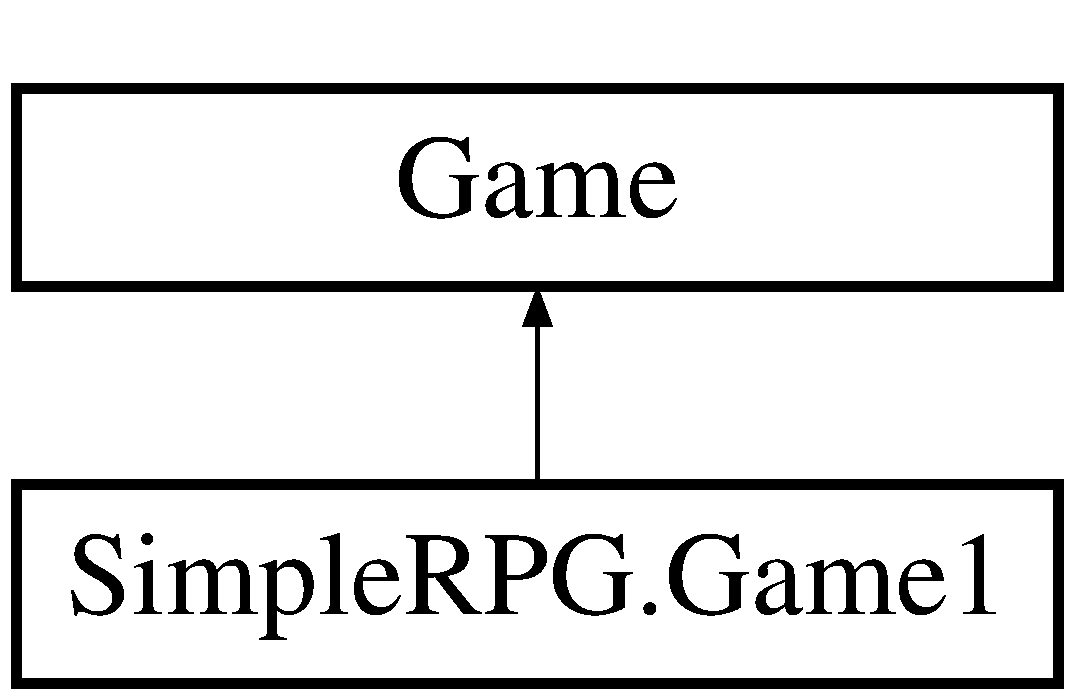
\includegraphics[height=2.000000cm]{class_simple_r_p_g_1_1_game1}
\end{center}
\end{figure}
\subsection*{Public Member Functions}
\begin{DoxyCompactItemize}
\item 
\hypertarget{class_simple_r_p_g_1_1_game1_aa58c4de2751f3b18058353f9e027eaf1}{\hyperlink{class_simple_r_p_g_1_1_states_1_1_game_state}{Game\-State} {\bfseries get\-First\-Game\-State} ()}\label{class_simple_r_p_g_1_1_game1_aa58c4de2751f3b18058353f9e027eaf1}

\item 
\hypertarget{class_simple_r_p_g_1_1_game1_acc5c4e36f80f0306fdafa3abb5846965}{int {\bfseries get\-Width} ()}\label{class_simple_r_p_g_1_1_game1_acc5c4e36f80f0306fdafa3abb5846965}

\item 
\hypertarget{class_simple_r_p_g_1_1_game1_acbd455c6801cd38476a757d40868d254}{int {\bfseries get\-Height} ()}\label{class_simple_r_p_g_1_1_game1_acbd455c6801cd38476a757d40868d254}

\item 
\hypertarget{class_simple_r_p_g_1_1_game1_a43306d1ac0dbb1e718127ece2b1e8c9e}{\hyperlink{class_simple_r_p_g_1_1_camera}{Camera} {\bfseries get\-Camera} ()}\label{class_simple_r_p_g_1_1_game1_a43306d1ac0dbb1e718127ece2b1e8c9e}

\item 
\hypertarget{class_simple_r_p_g_1_1_game1_a37252745c74499e7d63394079e7005a1}{int {\bfseries get\-Graphics\-Scale} ()}\label{class_simple_r_p_g_1_1_game1_a37252745c74499e7d63394079e7005a1}

\item 
\hypertarget{class_simple_r_p_g_1_1_game1_aabe60775a0239351456d6fd55eb1c838}{Sprite\-Font {\bfseries get\-Font} ()}\label{class_simple_r_p_g_1_1_game1_aabe60775a0239351456d6fd55eb1c838}

\end{DoxyCompactItemize}
\subsection*{Protected Member Functions}
\begin{DoxyCompactItemize}
\item 
override void \hyperlink{class_simple_r_p_g_1_1_game1_adb79c18a672c47805ed8e1ae2674b56a}{Initialize} ()
\begin{DoxyCompactList}\small\item\em Allows the game to perform any initialization it needs to before starting to run. This is where it can query for any required services and load any non-\/graphic related content. Calling base.\-Initialize will enumerate through any components and initialize them as well. \end{DoxyCompactList}\item 
override void \hyperlink{class_simple_r_p_g_1_1_game1_a2e98fc6671e04587ffec98ffcca94238}{Load\-Content} ()
\begin{DoxyCompactList}\small\item\em Load\-Content will be called once per game and is the place to load all of your content. \end{DoxyCompactList}\item 
override void \hyperlink{class_simple_r_p_g_1_1_game1_a59ed8cc0b068541b3d6193ca2b11fe87}{Unload\-Content} ()
\begin{DoxyCompactList}\small\item\em Unload\-Content will be called once per game and is the place to unload all content. \end{DoxyCompactList}\item 
override void \hyperlink{class_simple_r_p_g_1_1_game1_a85efe43ca6a5e6404743a8dc97dc3698}{Update} (Game\-Time game\-Time)
\begin{DoxyCompactList}\small\item\em Allows the game to run logic such as updating the world, checking for collisions, gathering input, and playing audio. \end{DoxyCompactList}\item 
override void \hyperlink{class_simple_r_p_g_1_1_game1_a6fdaff73ada28185db615d2eeae9bdfc}{Draw} (Game\-Time game\-Time)
\begin{DoxyCompactList}\small\item\em This is called when the game should draw itself. \end{DoxyCompactList}\end{DoxyCompactItemize}


\subsection{Detailed Description}
This is the main type for your game 



\subsection{Member Function Documentation}
\hypertarget{class_simple_r_p_g_1_1_game1_a6fdaff73ada28185db615d2eeae9bdfc}{\index{Simple\-R\-P\-G\-::\-Game1@{Simple\-R\-P\-G\-::\-Game1}!Draw@{Draw}}
\index{Draw@{Draw}!SimpleRPG::Game1@{Simple\-R\-P\-G\-::\-Game1}}
\subsubsection[{Draw}]{\setlength{\rightskip}{0pt plus 5cm}override void Simple\-R\-P\-G.\-Game1.\-Draw (
\begin{DoxyParamCaption}
\item[{Game\-Time}]{game\-Time}
\end{DoxyParamCaption}
)\hspace{0.3cm}{\ttfamily [inline]}, {\ttfamily [protected]}}}\label{class_simple_r_p_g_1_1_game1_a6fdaff73ada28185db615d2eeae9bdfc}


This is called when the game should draw itself. 


\begin{DoxyParams}{Parameters}
{\em game\-Time} & Provides a snapshot of timing values.\\
\hline
\end{DoxyParams}
\hypertarget{class_simple_r_p_g_1_1_game1_adb79c18a672c47805ed8e1ae2674b56a}{\index{Simple\-R\-P\-G\-::\-Game1@{Simple\-R\-P\-G\-::\-Game1}!Initialize@{Initialize}}
\index{Initialize@{Initialize}!SimpleRPG::Game1@{Simple\-R\-P\-G\-::\-Game1}}
\subsubsection[{Initialize}]{\setlength{\rightskip}{0pt plus 5cm}override void Simple\-R\-P\-G.\-Game1.\-Initialize (
\begin{DoxyParamCaption}
{}
\end{DoxyParamCaption}
)\hspace{0.3cm}{\ttfamily [inline]}, {\ttfamily [protected]}}}\label{class_simple_r_p_g_1_1_game1_adb79c18a672c47805ed8e1ae2674b56a}


Allows the game to perform any initialization it needs to before starting to run. This is where it can query for any required services and load any non-\/graphic related content. Calling base.\-Initialize will enumerate through any components and initialize them as well. 

\hypertarget{class_simple_r_p_g_1_1_game1_a2e98fc6671e04587ffec98ffcca94238}{\index{Simple\-R\-P\-G\-::\-Game1@{Simple\-R\-P\-G\-::\-Game1}!Load\-Content@{Load\-Content}}
\index{Load\-Content@{Load\-Content}!SimpleRPG::Game1@{Simple\-R\-P\-G\-::\-Game1}}
\subsubsection[{Load\-Content}]{\setlength{\rightskip}{0pt plus 5cm}override void Simple\-R\-P\-G.\-Game1.\-Load\-Content (
\begin{DoxyParamCaption}
{}
\end{DoxyParamCaption}
)\hspace{0.3cm}{\ttfamily [inline]}, {\ttfamily [protected]}}}\label{class_simple_r_p_g_1_1_game1_a2e98fc6671e04587ffec98ffcca94238}


Load\-Content will be called once per game and is the place to load all of your content. 

\hypertarget{class_simple_r_p_g_1_1_game1_a59ed8cc0b068541b3d6193ca2b11fe87}{\index{Simple\-R\-P\-G\-::\-Game1@{Simple\-R\-P\-G\-::\-Game1}!Unload\-Content@{Unload\-Content}}
\index{Unload\-Content@{Unload\-Content}!SimpleRPG::Game1@{Simple\-R\-P\-G\-::\-Game1}}
\subsubsection[{Unload\-Content}]{\setlength{\rightskip}{0pt plus 5cm}override void Simple\-R\-P\-G.\-Game1.\-Unload\-Content (
\begin{DoxyParamCaption}
{}
\end{DoxyParamCaption}
)\hspace{0.3cm}{\ttfamily [inline]}, {\ttfamily [protected]}}}\label{class_simple_r_p_g_1_1_game1_a59ed8cc0b068541b3d6193ca2b11fe87}


Unload\-Content will be called once per game and is the place to unload all content. 

\hypertarget{class_simple_r_p_g_1_1_game1_a85efe43ca6a5e6404743a8dc97dc3698}{\index{Simple\-R\-P\-G\-::\-Game1@{Simple\-R\-P\-G\-::\-Game1}!Update@{Update}}
\index{Update@{Update}!SimpleRPG::Game1@{Simple\-R\-P\-G\-::\-Game1}}
\subsubsection[{Update}]{\setlength{\rightskip}{0pt plus 5cm}override void Simple\-R\-P\-G.\-Game1.\-Update (
\begin{DoxyParamCaption}
\item[{Game\-Time}]{game\-Time}
\end{DoxyParamCaption}
)\hspace{0.3cm}{\ttfamily [inline]}, {\ttfamily [protected]}}}\label{class_simple_r_p_g_1_1_game1_a85efe43ca6a5e6404743a8dc97dc3698}


Allows the game to run logic such as updating the world, checking for collisions, gathering input, and playing audio. 


\begin{DoxyParams}{Parameters}
{\em game\-Time} & Provides a snapshot of timing values.\\
\hline
\end{DoxyParams}


The documentation for this class was generated from the following file\-:\begin{DoxyCompactItemize}
\item 
Simple\-R\-P\-G/\-Simple\-R\-P\-G/Game1.\-cs\end{DoxyCompactItemize}

\hypertarget{class_simple_r_p_g_1_1_states_1_1_game_state}{\section{Simple\+R\+P\+G.\+States.\+Game\+State Class Reference}
\label{class_simple_r_p_g_1_1_states_1_1_game_state}\index{Simple\+R\+P\+G.\+States.\+Game\+State@{Simple\+R\+P\+G.\+States.\+Game\+State}}
}
Inheritance diagram for Simple\+R\+P\+G.\+States.\+Game\+State\+:\begin{figure}[H]
\begin{center}
\leavevmode
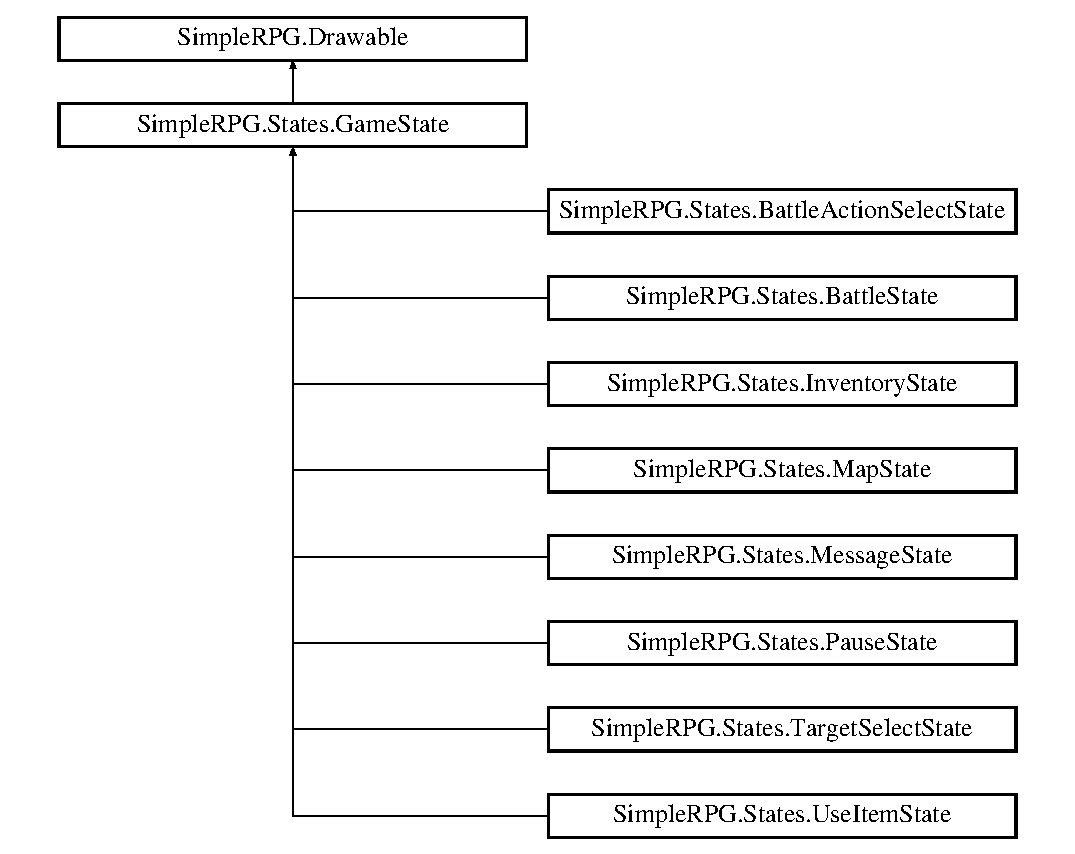
\includegraphics[height=10.000000cm]{class_simple_r_p_g_1_1_states_1_1_game_state}
\end{center}
\end{figure}
\subsection*{Public Member Functions}
\begin{DoxyCompactItemize}
\item 
\hypertarget{class_simple_r_p_g_1_1_states_1_1_game_state_a0739c91318628b0180c6039558fdaf59}{{\bfseries Game\+State} (\hyperlink{class_simple_r_p_g_1_1_game1}{Game1} game, \hyperlink{class_simple_r_p_g_1_1_states_1_1_game_state}{Game\+State} parent, \hyperlink{class_simple_r_p_g_1_1_states_1_1_state_manager}{State\+Manager} manager)}\label{class_simple_r_p_g_1_1_states_1_1_game_state_a0739c91318628b0180c6039558fdaf59}

\item 
\hypertarget{class_simple_r_p_g_1_1_states_1_1_game_state_ac89d802264bde3ba8d889375f413e4ea}{override void {\bfseries update} ()}\label{class_simple_r_p_g_1_1_states_1_1_game_state_ac89d802264bde3ba8d889375f413e4ea}

\item 
\hypertarget{class_simple_r_p_g_1_1_states_1_1_game_state_a0c2042a1d0c61f53d630c4befbb130b9}{virtual void {\bfseries draw} (Sprite\+Batch sprite\+Batch)}\label{class_simple_r_p_g_1_1_states_1_1_game_state_a0c2042a1d0c61f53d630c4befbb130b9}

\item 
\hypertarget{class_simple_r_p_g_1_1_states_1_1_game_state_a52586b02847099e993bb3acd30f996a5}{virtual void {\bfseries exit} ()}\label{class_simple_r_p_g_1_1_states_1_1_game_state_a52586b02847099e993bb3acd30f996a5}

\item 
\hypertarget{class_simple_r_p_g_1_1_states_1_1_game_state_a2a3a4da7363acb938403f669517b9de0}{void {\bfseries add\+Child\+State} (\hyperlink{class_simple_r_p_g_1_1_states_1_1_game_state}{Game\+State} state)}\label{class_simple_r_p_g_1_1_states_1_1_game_state_a2a3a4da7363acb938403f669517b9de0}

\end{DoxyCompactItemize}
\subsection*{Protected Member Functions}
\begin{DoxyCompactItemize}
\item 
\hypertarget{class_simple_r_p_g_1_1_states_1_1_game_state_aec6e20917880e857868ac584906515c6}{virtual void {\bfseries pass\+Data} (\hyperlink{class_simple_r_p_g_1_1_states_1_1_game_state}{Game\+State} sender, object data)}\label{class_simple_r_p_g_1_1_states_1_1_game_state_aec6e20917880e857868ac584906515c6}

\end{DoxyCompactItemize}
\subsection*{Protected Attributes}
\begin{DoxyCompactItemize}
\item 
\hypertarget{class_simple_r_p_g_1_1_states_1_1_game_state_abebc6e51f9c375485bc03185a466fe4b}{\hyperlink{class_simple_r_p_g_1_1_game1}{Game1} {\bfseries game\+Ref}}\label{class_simple_r_p_g_1_1_states_1_1_game_state_abebc6e51f9c375485bc03185a466fe4b}

\item 
\hypertarget{class_simple_r_p_g_1_1_states_1_1_game_state_a7ede7a30255b2894fee92cd3dcb9b5fe}{\hyperlink{class_simple_r_p_g_1_1_states_1_1_state_manager}{State\+Manager} {\bfseries state\+Manager}}\label{class_simple_r_p_g_1_1_states_1_1_game_state_a7ede7a30255b2894fee92cd3dcb9b5fe}

\item 
\hypertarget{class_simple_r_p_g_1_1_states_1_1_game_state_ada3000d2cec329e802a0693e2a2a8281}{bool {\bfseries pop\+On\+Escape} = true}\label{class_simple_r_p_g_1_1_states_1_1_game_state_ada3000d2cec329e802a0693e2a2a8281}

\item 
\hypertarget{class_simple_r_p_g_1_1_states_1_1_game_state_a03c7c40f61ca5893d6e5a106e9d9d5a8}{Animation\+Type {\bfseries in\+Animation} = Animation\+Type.\+Fade}\label{class_simple_r_p_g_1_1_states_1_1_game_state_a03c7c40f61ca5893d6e5a106e9d9d5a8}

\item 
\hypertarget{class_simple_r_p_g_1_1_states_1_1_game_state_a3cb05ec585e6744764a94f160efe05ab}{bool {\bfseries closing} = false}\label{class_simple_r_p_g_1_1_states_1_1_game_state_a3cb05ec585e6744764a94f160efe05ab}

\item 
\hypertarget{class_simple_r_p_g_1_1_states_1_1_game_state_a24084ddfaff8f9469c7432fb4be05a1e}{\hyperlink{class_simple_r_p_g_1_1_states_1_1_game_state}{Game\+State} {\bfseries parent\+State}}\label{class_simple_r_p_g_1_1_states_1_1_game_state_a24084ddfaff8f9469c7432fb4be05a1e}

\end{DoxyCompactItemize}


The documentation for this class was generated from the following file\+:\begin{DoxyCompactItemize}
\item 
D\+:/\+Dropbox/\+Simple\+R\+P\+G/\+Simple\+R\+P\+G/\+Simple\+R\+P\+G/\+States/Game\+State.\+cs\end{DoxyCompactItemize}

\hypertarget{class_simple_r_p_g_1_1_input}{\section{Simple\-R\-P\-G.\-Input Class Reference}
\label{class_simple_r_p_g_1_1_input}\index{Simple\-R\-P\-G.\-Input@{Simple\-R\-P\-G.\-Input}}
}
\subsection*{Static Public Member Functions}
\begin{DoxyCompactItemize}
\item 
\hypertarget{class_simple_r_p_g_1_1_input_a5030a4e61c1ca8fc490575e968339126}{static void {\bfseries update} ()}\label{class_simple_r_p_g_1_1_input_a5030a4e61c1ca8fc490575e968339126}

\item 
\hypertarget{class_simple_r_p_g_1_1_input_a187b5eab7cd9b9f198adb08d7a507b3c}{static bool {\bfseries is\-Key\-Down} (Keys key)}\label{class_simple_r_p_g_1_1_input_a187b5eab7cd9b9f198adb08d7a507b3c}

\item 
\hypertarget{class_simple_r_p_g_1_1_input_ab67cea9332b183fb664d9bf497ad61c6}{static bool {\bfseries is\-Key\-Pressed} (Keys key)}\label{class_simple_r_p_g_1_1_input_ab67cea9332b183fb664d9bf497ad61c6}

\item 
\hypertarget{class_simple_r_p_g_1_1_input_aa2424d5308db570017de73a616ad48eb}{static bool {\bfseries is\-Key\-Released} (Keys key)}\label{class_simple_r_p_g_1_1_input_aa2424d5308db570017de73a616ad48eb}

\item 
\hypertarget{class_simple_r_p_g_1_1_input_a70cff65ec2b3d91956952a1986fa22d6}{static Vector2 {\bfseries get\-Mouse\-Position} ()}\label{class_simple_r_p_g_1_1_input_a70cff65ec2b3d91956952a1986fa22d6}

\end{DoxyCompactItemize}


The documentation for this class was generated from the following file\-:\begin{DoxyCompactItemize}
\item 
Simple\-R\-P\-G/\-Simple\-R\-P\-G/Input.\-cs\end{DoxyCompactItemize}

\hypertarget{class_simple_r_p_g_1_1_states_1_1_inventory_state}{\section{Simple\+R\+P\+G.\+States.\+Inventory\+State Class Reference}
\label{class_simple_r_p_g_1_1_states_1_1_inventory_state}\index{Simple\+R\+P\+G.\+States.\+Inventory\+State@{Simple\+R\+P\+G.\+States.\+Inventory\+State}}
}
Inheritance diagram for Simple\+R\+P\+G.\+States.\+Inventory\+State\+:\begin{figure}[H]
\begin{center}
\leavevmode
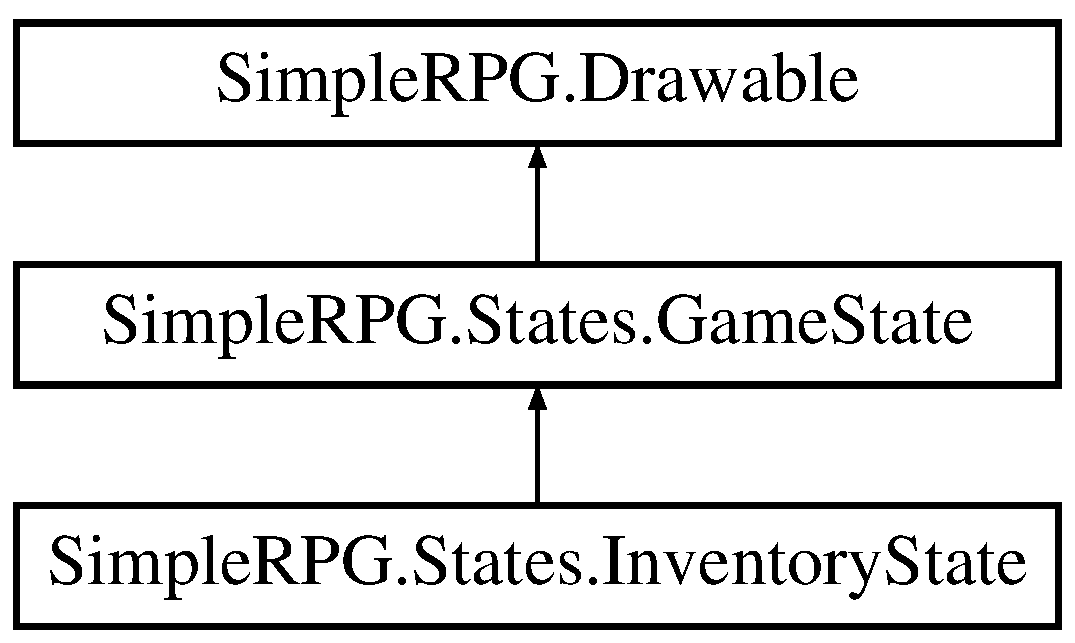
\includegraphics[height=3.000000cm]{class_simple_r_p_g_1_1_states_1_1_inventory_state}
\end{center}
\end{figure}
\subsection*{Public Member Functions}
\begin{DoxyCompactItemize}
\item 
\hypertarget{class_simple_r_p_g_1_1_states_1_1_inventory_state_aeed5770ba4e1f6d9a4c132d2fb1b71f1}{{\bfseries Inventory\+State} (\hyperlink{class_simple_r_p_g_1_1_game1}{Game1} game, \hyperlink{class_simple_r_p_g_1_1_states_1_1_state_manager}{State\+Manager} manager, \hyperlink{class_simple_r_p_g_1_1_states_1_1_game_state}{Game\+State} parent, Point window\+Position)}\label{class_simple_r_p_g_1_1_states_1_1_inventory_state_aeed5770ba4e1f6d9a4c132d2fb1b71f1}

\item 
\hypertarget{class_simple_r_p_g_1_1_states_1_1_inventory_state_a87827673a8facbdc18bbe4de68eb250b}{override void {\bfseries update} ()}\label{class_simple_r_p_g_1_1_states_1_1_inventory_state_a87827673a8facbdc18bbe4de68eb250b}

\item 
\hypertarget{class_simple_r_p_g_1_1_states_1_1_inventory_state_a1632dd2d7dba038d8416130ef4e7e643}{override void {\bfseries exit} ()}\label{class_simple_r_p_g_1_1_states_1_1_inventory_state_a1632dd2d7dba038d8416130ef4e7e643}

\item 
\hypertarget{class_simple_r_p_g_1_1_states_1_1_inventory_state_a1a7b78358df3cc6c9e21084195f1c99e}{override void {\bfseries draw} (Sprite\+Batch sprite\+Batch)}\label{class_simple_r_p_g_1_1_states_1_1_inventory_state_a1a7b78358df3cc6c9e21084195f1c99e}

\end{DoxyCompactItemize}
\subsection*{Protected Attributes}
\begin{DoxyCompactItemize}
\item 
\hypertarget{class_simple_r_p_g_1_1_states_1_1_inventory_state_aa5316f2c76266582d48e44d711d484d8}{\hyperlink{class_simple_r_p_g_1_1_item_container}{Item\+Container} {\bfseries player\+Inventory}}\label{class_simple_r_p_g_1_1_states_1_1_inventory_state_aa5316f2c76266582d48e44d711d484d8}

\item 
\hypertarget{class_simple_r_p_g_1_1_states_1_1_inventory_state_ade61f6d43d5d01beaf81c2542f6a4c80}{\hyperlink{class_simple_r_p_g_1_1_windows_1_1_item_list}{Item\+List} {\bfseries item\+List}}\label{class_simple_r_p_g_1_1_states_1_1_inventory_state_ade61f6d43d5d01beaf81c2542f6a4c80}

\item 
\hypertarget{class_simple_r_p_g_1_1_states_1_1_inventory_state_a82b7015c1fd0c9f7f79bb8eb20f63959}{\hyperlink{class_simple_r_p_g_1_1_windows_1_1_item_description_window}{Item\+Description\+Window} {\bfseries description\+Window}}\label{class_simple_r_p_g_1_1_states_1_1_inventory_state_a82b7015c1fd0c9f7f79bb8eb20f63959}

\end{DoxyCompactItemize}
\subsection*{Additional Inherited Members}


The documentation for this class was generated from the following file\+:\begin{DoxyCompactItemize}
\item 
D\+:/\+Dropbox/\+Simple\+R\+P\+G/\+Simple\+R\+P\+G/\+Simple\+R\+P\+G/\+States/Inventory\+State.\+cs\end{DoxyCompactItemize}

\hypertarget{class_simple_r_p_g_1_1_item}{\section{Simple\+R\+P\+G.\+Item Class Reference}
\label{class_simple_r_p_g_1_1_item}\index{Simple\+R\+P\+G.\+Item@{Simple\+R\+P\+G.\+Item}}
}
\subsection*{Public Member Functions}
\begin{DoxyCompactItemize}
\item 
\hypertarget{class_simple_r_p_g_1_1_item_a63d4839f76cceeb7f531c6ff5843993c}{{\bfseries Item} (string item\+Name, string item\+Description)}\label{class_simple_r_p_g_1_1_item_a63d4839f76cceeb7f531c6ff5843993c}

\item 
\hypertarget{class_simple_r_p_g_1_1_item_a7389a06ee32aa5f6bd22087a660b642f}{string {\bfseries get\+Name} ()}\label{class_simple_r_p_g_1_1_item_a7389a06ee32aa5f6bd22087a660b642f}

\item 
\hypertarget{class_simple_r_p_g_1_1_item_a4e5a4789bbbf66b9881afe307e971449}{string {\bfseries get\+Description} ()}\label{class_simple_r_p_g_1_1_item_a4e5a4789bbbf66b9881afe307e971449}

\item 
\hypertarget{class_simple_r_p_g_1_1_item_a82dba77a31a3d0898ea32a1f8ad1d8f6}{\hyperlink{class_simple_r_p_g_1_1_item}{Item} {\bfseries clone} ()}\label{class_simple_r_p_g_1_1_item_a82dba77a31a3d0898ea32a1f8ad1d8f6}

\end{DoxyCompactItemize}
\subsection*{Protected Attributes}
\begin{DoxyCompactItemize}
\item 
\hypertarget{class_simple_r_p_g_1_1_item_ad3f8fe06680aa41d2e8b09860ca8c9b5}{string {\bfseries name}}\label{class_simple_r_p_g_1_1_item_ad3f8fe06680aa41d2e8b09860ca8c9b5}

\item 
\hypertarget{class_simple_r_p_g_1_1_item_ad311fedc8d5f53b55f4053de21cb58b0}{Texture2\+D {\bfseries icon}}\label{class_simple_r_p_g_1_1_item_ad311fedc8d5f53b55f4053de21cb58b0}

\end{DoxyCompactItemize}


The documentation for this class was generated from the following file\+:\begin{DoxyCompactItemize}
\item 
D\+:/\+Dropbox/\+Simple\+R\+P\+G/\+Simple\+R\+P\+G/\+Simple\+R\+P\+G/Item.\+cs\end{DoxyCompactItemize}

\hypertarget{class_simple_r_p_g_1_1_item_container}{\section{Simple\+R\+P\+G.\+Item\+Container Class Reference}
\label{class_simple_r_p_g_1_1_item_container}\index{Simple\+R\+P\+G.\+Item\+Container@{Simple\+R\+P\+G.\+Item\+Container}}
}
\subsection*{Public Member Functions}
\begin{DoxyCompactItemize}
\item 
\hypertarget{class_simple_r_p_g_1_1_item_container_af7845137ba10a262ec241c5c7d0176b3}{bool {\bfseries contains} (\hyperlink{class_simple_r_p_g_1_1_item}{Item} item)}\label{class_simple_r_p_g_1_1_item_container_af7845137ba10a262ec241c5c7d0176b3}

\item 
\hypertarget{class_simple_r_p_g_1_1_item_container_ac7d2bf711fd35c069ed0c6fca9286186}{bool {\bfseries contains} (string item\+Name)}\label{class_simple_r_p_g_1_1_item_container_ac7d2bf711fd35c069ed0c6fca9286186}

\item 
\hypertarget{class_simple_r_p_g_1_1_item_container_abe794c84a443d0cc5b2a93ca766982f1}{int {\bfseries number\+Of\+Item} (\hyperlink{class_simple_r_p_g_1_1_item}{Item} item)}\label{class_simple_r_p_g_1_1_item_container_abe794c84a443d0cc5b2a93ca766982f1}

\item 
\hypertarget{class_simple_r_p_g_1_1_item_container_af0fceaa5260f3e0e342a9c6ea2dd14b8}{int {\bfseries number\+Of\+Item} (string item\+Name)}\label{class_simple_r_p_g_1_1_item_container_af0fceaa5260f3e0e342a9c6ea2dd14b8}

\item 
\hypertarget{class_simple_r_p_g_1_1_item_container_a83f030ff97e9609c60f46f98ea530acd}{void {\bfseries add\+Item} (\hyperlink{class_simple_r_p_g_1_1_item}{Item} item)}\label{class_simple_r_p_g_1_1_item_container_a83f030ff97e9609c60f46f98ea530acd}

\item 
\hypertarget{class_simple_r_p_g_1_1_item_container_a2ee46a7efb27787692534b528dbb9ae4}{void {\bfseries add\+Item} (string item\+Name)}\label{class_simple_r_p_g_1_1_item_container_a2ee46a7efb27787692534b528dbb9ae4}

\item 
\hypertarget{class_simple_r_p_g_1_1_item_container_adbcd58034e8002b2de9e187a03096d9f}{void {\bfseries remove\+Item} (\hyperlink{class_simple_r_p_g_1_1_item}{Item} item)}\label{class_simple_r_p_g_1_1_item_container_adbcd58034e8002b2de9e187a03096d9f}

\item 
\hypertarget{class_simple_r_p_g_1_1_item_container_af25b73361cb340c7d269d7899e298863}{void {\bfseries remove\+Item} (string item\+Name)}\label{class_simple_r_p_g_1_1_item_container_af25b73361cb340c7d269d7899e298863}

\item 
\hypertarget{class_simple_r_p_g_1_1_item_container_ad2e359e69ee0ce1803484a5e2297c832}{int {\bfseries count} ()}\label{class_simple_r_p_g_1_1_item_container_ad2e359e69ee0ce1803484a5e2297c832}

\item 
\hypertarget{class_simple_r_p_g_1_1_item_container_a70f22b47613da478f2d214c01fc2155a}{string\mbox{[}$\,$\mbox{]} {\bfseries get\+Item\+Names} ()}\label{class_simple_r_p_g_1_1_item_container_a70f22b47613da478f2d214c01fc2155a}

\end{DoxyCompactItemize}
\subsection*{Protected Attributes}
\begin{DoxyCompactItemize}
\item 
\hypertarget{class_simple_r_p_g_1_1_item_container_a0034a3a35d900ba8998929555c8d7dcf}{Dictionary$<$ string, int $>$ {\bfseries item\+Quantities}}\label{class_simple_r_p_g_1_1_item_container_a0034a3a35d900ba8998929555c8d7dcf}

\end{DoxyCompactItemize}


The documentation for this class was generated from the following file\+:\begin{DoxyCompactItemize}
\item 
D\+:/\+Dropbox/\+Simple\+R\+P\+G/\+Simple\+R\+P\+G/\+Simple\+R\+P\+G/Item\+Container.\+cs\end{DoxyCompactItemize}

\hypertarget{class_simple_r_p_g_1_1_windows_1_1_item_description_window}{\section{Simple\-R\-P\-G.\-Windows.\-Item\-Description\-Window Class Reference}
\label{class_simple_r_p_g_1_1_windows_1_1_item_description_window}\index{Simple\-R\-P\-G.\-Windows.\-Item\-Description\-Window@{Simple\-R\-P\-G.\-Windows.\-Item\-Description\-Window}}
}
Inheritance diagram for Simple\-R\-P\-G.\-Windows.\-Item\-Description\-Window\-:\begin{figure}[H]
\begin{center}
\leavevmode
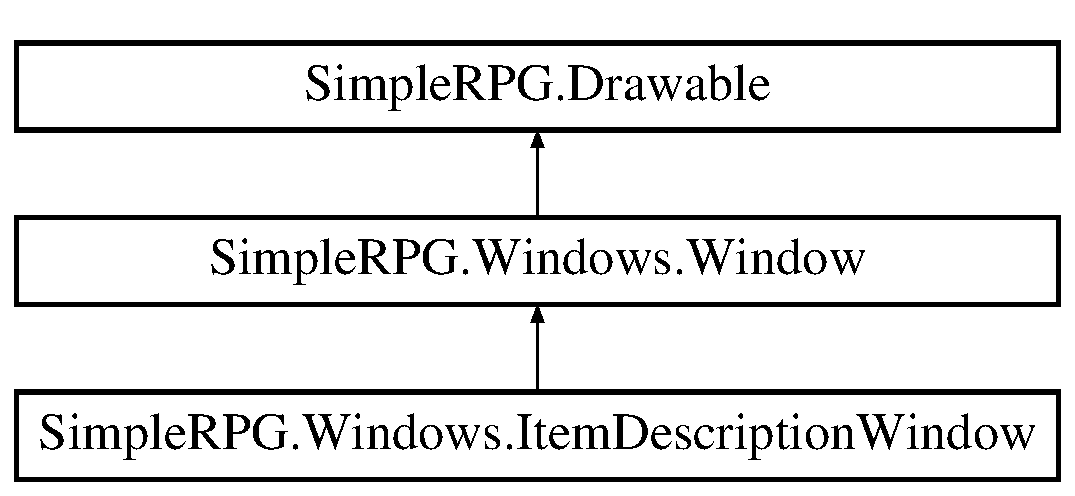
\includegraphics[height=3.000000cm]{class_simple_r_p_g_1_1_windows_1_1_item_description_window}
\end{center}
\end{figure}
\subsection*{Public Member Functions}
\begin{DoxyCompactItemize}
\item 
\hypertarget{class_simple_r_p_g_1_1_windows_1_1_item_description_window_a632484e7c47d19555b68a43c7ef314b1}{{\bfseries Item\-Description\-Window} (\hyperlink{class_simple_r_p_g_1_1_game1}{Game1} game, Point req\-Position, int req\-Width, int req\-Height)}\label{class_simple_r_p_g_1_1_windows_1_1_item_description_window_a632484e7c47d19555b68a43c7ef314b1}

\item 
\hypertarget{class_simple_r_p_g_1_1_windows_1_1_item_description_window_a5346e4574e7a29a3a09cbde41e523fbe}{override void {\bfseries draw} (Sprite\-Batch sprite\-Batch)}\label{class_simple_r_p_g_1_1_windows_1_1_item_description_window_a5346e4574e7a29a3a09cbde41e523fbe}

\item 
\hypertarget{class_simple_r_p_g_1_1_windows_1_1_item_description_window_aec5da8cb493b5960a6cda6d5ec10610d}{void {\bfseries set\-Description} (string new\-Description)}\label{class_simple_r_p_g_1_1_windows_1_1_item_description_window_aec5da8cb493b5960a6cda6d5ec10610d}

\end{DoxyCompactItemize}
\subsection*{Protected Attributes}
\begin{DoxyCompactItemize}
\item 
\hypertarget{class_simple_r_p_g_1_1_windows_1_1_item_description_window_ac9367e28041ff7f0bfa406bd8d3e49b3}{string {\bfseries description} = \char`\"{}\char`\"{}}\label{class_simple_r_p_g_1_1_windows_1_1_item_description_window_ac9367e28041ff7f0bfa406bd8d3e49b3}

\end{DoxyCompactItemize}


The documentation for this class was generated from the following file\-:\begin{DoxyCompactItemize}
\item 
Simple\-R\-P\-G/\-Simple\-R\-P\-G/\-Windows/Item\-Description\-Window.\-cs\end{DoxyCompactItemize}

\hypertarget{class_simple_r_p_g_1_1_windows_1_1_item_list}{\section{Simple\+R\+P\+G.\+Windows.\+Item\+List Class Reference}
\label{class_simple_r_p_g_1_1_windows_1_1_item_list}\index{Simple\+R\+P\+G.\+Windows.\+Item\+List@{Simple\+R\+P\+G.\+Windows.\+Item\+List}}
}
Inheritance diagram for Simple\+R\+P\+G.\+Windows.\+Item\+List\+:\begin{figure}[H]
\begin{center}
\leavevmode
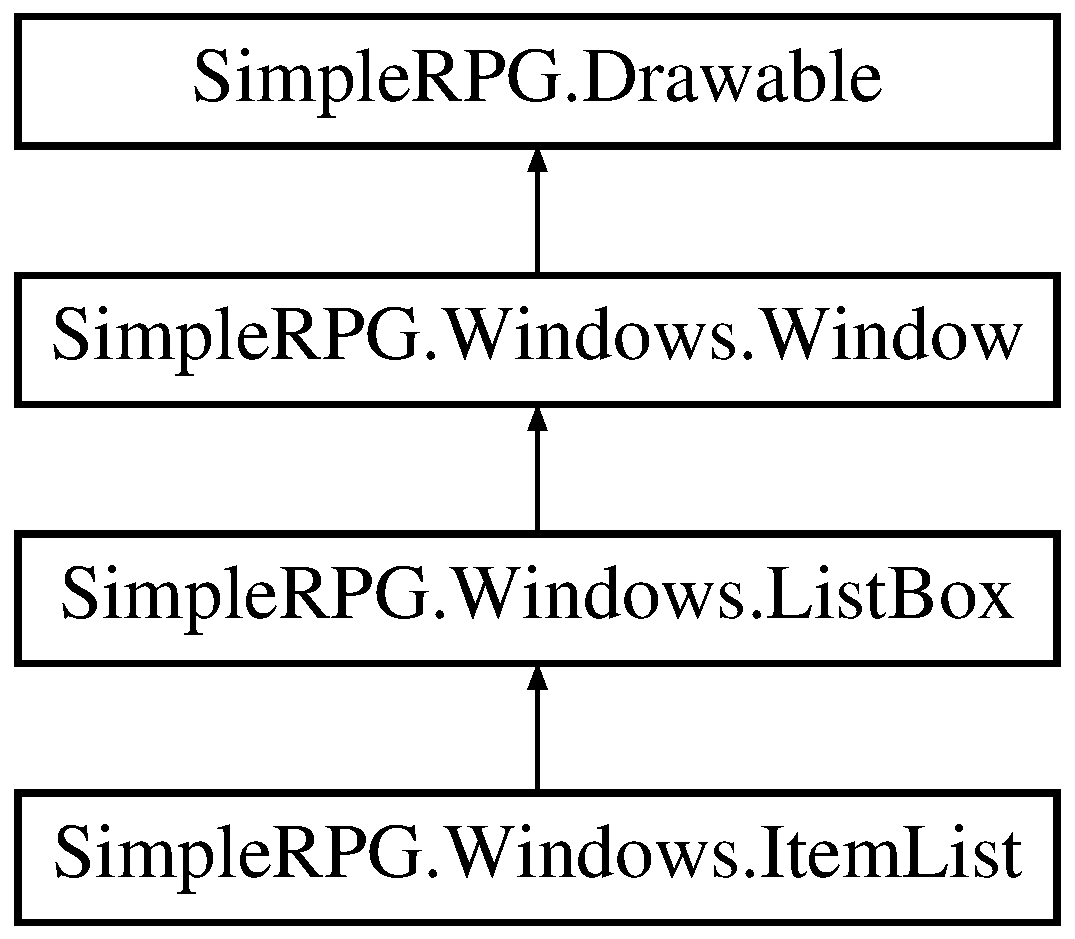
\includegraphics[height=4.000000cm]{class_simple_r_p_g_1_1_windows_1_1_item_list}
\end{center}
\end{figure}
\subsection*{Public Member Functions}
\begin{DoxyCompactItemize}
\item 
\hypertarget{class_simple_r_p_g_1_1_windows_1_1_item_list_a18f5608d7498c2c0bcefd449853a67cc}{{\bfseries Item\+List} (\hyperlink{class_simple_r_p_g_1_1_game1}{Game1} game, Point req\+Position, int req\+Width, int options\+In\+Window, \hyperlink{class_simple_r_p_g_1_1_item_container}{Item\+Container} items)}\label{class_simple_r_p_g_1_1_windows_1_1_item_list_a18f5608d7498c2c0bcefd449853a67cc}

\item 
\hypertarget{class_simple_r_p_g_1_1_windows_1_1_item_list_a3e66f13e5441ede760ea0354dcad386b}{\hyperlink{class_simple_r_p_g_1_1_item}{Item} {\bfseries get\+Selected\+Item} ()}\label{class_simple_r_p_g_1_1_windows_1_1_item_list_a3e66f13e5441ede760ea0354dcad386b}

\end{DoxyCompactItemize}
\subsection*{Protected Member Functions}
\begin{DoxyCompactItemize}
\item 
\hypertarget{class_simple_r_p_g_1_1_windows_1_1_item_list_a1a0df2d3034a3ce9dd2e98f6a1a0aed6}{override void {\bfseries draw\+Options} (Sprite\+Batch sprite\+Batch)}\label{class_simple_r_p_g_1_1_windows_1_1_item_list_a1a0df2d3034a3ce9dd2e98f6a1a0aed6}

\end{DoxyCompactItemize}
\subsection*{Protected Attributes}
\begin{DoxyCompactItemize}
\item 
\hypertarget{class_simple_r_p_g_1_1_windows_1_1_item_list_a85d047fe8d365e9be51af2f59dc47782}{\hyperlink{class_simple_r_p_g_1_1_item_container}{Item\+Container} {\bfseries item\+Container}}\label{class_simple_r_p_g_1_1_windows_1_1_item_list_a85d047fe8d365e9be51af2f59dc47782}

\end{DoxyCompactItemize}


The documentation for this class was generated from the following file\+:\begin{DoxyCompactItemize}
\item 
D\+:/\+Dropbox/\+Simple\+R\+P\+G/\+Simple\+R\+P\+G/\+Simple\+R\+P\+G/\+Windows/Item\+List.\+cs\end{DoxyCompactItemize}

\hypertarget{class_simple_r_p_g_1_1_item_manager}{\section{Simple\+R\+P\+G.\+Item\+Manager Class Reference}
\label{class_simple_r_p_g_1_1_item_manager}\index{Simple\+R\+P\+G.\+Item\+Manager@{Simple\+R\+P\+G.\+Item\+Manager}}
}
\subsection*{Static Public Member Functions}
\begin{DoxyCompactItemize}
\item 
\hypertarget{class_simple_r_p_g_1_1_item_manager_a50b3096096d3181934d872b5b96a0477}{static void {\bfseries add\+New\+Item} (\hyperlink{class_simple_r_p_g_1_1_item}{Item} item)}\label{class_simple_r_p_g_1_1_item_manager_a50b3096096d3181934d872b5b96a0477}

\item 
\hypertarget{class_simple_r_p_g_1_1_item_manager_a1bed1b8f2d71a468934d1b652f14e711}{static \hyperlink{class_simple_r_p_g_1_1_item}{Item} {\bfseries get\+Item} (string item\+Name)}\label{class_simple_r_p_g_1_1_item_manager_a1bed1b8f2d71a468934d1b652f14e711}

\item 
\hypertarget{class_simple_r_p_g_1_1_item_manager_a2a9850af52bb4675e337d344e570a5e1}{static void {\bfseries initialize} ()}\label{class_simple_r_p_g_1_1_item_manager_a2a9850af52bb4675e337d344e570a5e1}

\end{DoxyCompactItemize}


The documentation for this class was generated from the following file\+:\begin{DoxyCompactItemize}
\item 
D\+:/\+Dropbox/\+Simple\+R\+P\+G/\+Simple\+R\+P\+G/\+Simple\+R\+P\+G/Item\+Manager.\+cs\end{DoxyCompactItemize}

\hypertarget{class_simple_r_p_g_1_1_windows_1_1_list_box}{\section{Simple\-R\-P\-G.\-Windows.\-List\-Box Class Reference}
\label{class_simple_r_p_g_1_1_windows_1_1_list_box}\index{Simple\-R\-P\-G.\-Windows.\-List\-Box@{Simple\-R\-P\-G.\-Windows.\-List\-Box}}
}
Inheritance diagram for Simple\-R\-P\-G.\-Windows.\-List\-Box\-:\begin{figure}[H]
\begin{center}
\leavevmode
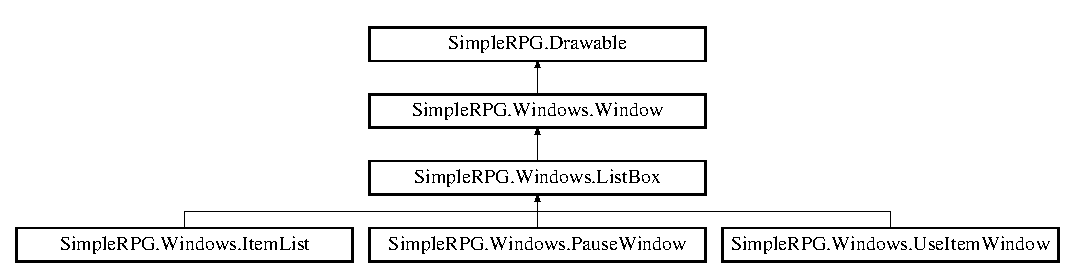
\includegraphics[height=2.362869cm]{class_simple_r_p_g_1_1_windows_1_1_list_box}
\end{center}
\end{figure}
\subsection*{Public Member Functions}
\begin{DoxyCompactItemize}
\item 
\hypertarget{class_simple_r_p_g_1_1_windows_1_1_list_box_adb75959fbbfaad12d00d92ea25df02fd}{{\bfseries List\-Box} (\hyperlink{class_simple_r_p_g_1_1_game1}{Game1} game, Point req\-Position, int req\-Width, int options\-In\-Window, string\mbox{[}$\,$\mbox{]} items, string windowskin)}\label{class_simple_r_p_g_1_1_windows_1_1_list_box_adb75959fbbfaad12d00d92ea25df02fd}

\item 
\hypertarget{class_simple_r_p_g_1_1_windows_1_1_list_box_a9554b0fc0656571c97d4b633dd63f4c0}{override void {\bfseries draw} (Sprite\-Batch sprite\-Batch)}\label{class_simple_r_p_g_1_1_windows_1_1_list_box_a9554b0fc0656571c97d4b633dd63f4c0}

\item 
\hypertarget{class_simple_r_p_g_1_1_windows_1_1_list_box_ae061189951387436b8d0edc90e667330}{override void {\bfseries update} ()}\label{class_simple_r_p_g_1_1_windows_1_1_list_box_ae061189951387436b8d0edc90e667330}

\item 
\hypertarget{class_simple_r_p_g_1_1_windows_1_1_list_box_a70ee330db8b560653f784c5cadbad07c}{void {\bfseries set\-Options} (string\mbox{[}$\,$\mbox{]} items, bool\mbox{[}$\,$\mbox{]} enabled)}\label{class_simple_r_p_g_1_1_windows_1_1_list_box_a70ee330db8b560653f784c5cadbad07c}

\item 
\hypertarget{class_simple_r_p_g_1_1_windows_1_1_list_box_a3b6d40c01a1c816fc7e72aea2e6d328a}{void {\bfseries set\-Options} (string\mbox{[}$\,$\mbox{]} items)}\label{class_simple_r_p_g_1_1_windows_1_1_list_box_a3b6d40c01a1c816fc7e72aea2e6d328a}

\item 
\hypertarget{class_simple_r_p_g_1_1_windows_1_1_list_box_aa9dd5bf1dc7b9440a12ec386280f50dd}{void {\bfseries set\-Index\-Enable\-State} (int temp\-Index, bool new\-State)}\label{class_simple_r_p_g_1_1_windows_1_1_list_box_aa9dd5bf1dc7b9440a12ec386280f50dd}

\item 
\hypertarget{class_simple_r_p_g_1_1_windows_1_1_list_box_aa7f9529f9103613c7743ea4507da0308}{void {\bfseries set\-Enabled\-Options} (bool\mbox{[}$\,$\mbox{]} enabled)}\label{class_simple_r_p_g_1_1_windows_1_1_list_box_aa7f9529f9103613c7743ea4507da0308}

\item 
\hypertarget{class_simple_r_p_g_1_1_windows_1_1_list_box_a4abd9037503be834ae7a194bd1449999}{int {\bfseries get\-Index} ()}\label{class_simple_r_p_g_1_1_windows_1_1_list_box_a4abd9037503be834ae7a194bd1449999}

\item 
\hypertarget{class_simple_r_p_g_1_1_windows_1_1_list_box_a830d5ae33e0866b2f2c9c712cec51510}{void {\bfseries set\-Text\-Align} (\hyperlink{namespace_simple_r_p_g_a956c6a011833191ccb1b0aa38a1d5916}{Text\-Align} new\-Alignment)}\label{class_simple_r_p_g_1_1_windows_1_1_list_box_a830d5ae33e0866b2f2c9c712cec51510}

\end{DoxyCompactItemize}
\subsection*{Protected Member Functions}
\begin{DoxyCompactItemize}
\item 
\hypertarget{class_simple_r_p_g_1_1_windows_1_1_list_box_a210c6cdcd777e69676153e318e2cf565}{void {\bfseries set\-First\-Index} ()}\label{class_simple_r_p_g_1_1_windows_1_1_list_box_a210c6cdcd777e69676153e318e2cf565}

\item 
\hypertarget{class_simple_r_p_g_1_1_windows_1_1_list_box_a2005eacdc6532a13a25933f880e5ede1}{virtual void {\bfseries draw\-Options} (Sprite\-Batch sprite\-Batch)}\label{class_simple_r_p_g_1_1_windows_1_1_list_box_a2005eacdc6532a13a25933f880e5ede1}

\item 
\hypertarget{class_simple_r_p_g_1_1_windows_1_1_list_box_a4c2195c09a0f158c667c7cfcf802ff48}{void {\bfseries move\-Cursor\-Down} ()}\label{class_simple_r_p_g_1_1_windows_1_1_list_box_a4c2195c09a0f158c667c7cfcf802ff48}

\item 
\hypertarget{class_simple_r_p_g_1_1_windows_1_1_list_box_a499a5c3c093ceae369ab8572cad411ab}{void {\bfseries move\-Cursor\-Up} ()}\label{class_simple_r_p_g_1_1_windows_1_1_list_box_a499a5c3c093ceae369ab8572cad411ab}

\end{DoxyCompactItemize}
\subsection*{Protected Attributes}
\begin{DoxyCompactItemize}
\item 
\hypertarget{class_simple_r_p_g_1_1_windows_1_1_list_box_a92c83b7cef9c2dfc6a73d7eff0452f4b}{List$<$ string $>$ {\bfseries options}}\label{class_simple_r_p_g_1_1_windows_1_1_list_box_a92c83b7cef9c2dfc6a73d7eff0452f4b}

\item 
\hypertarget{class_simple_r_p_g_1_1_windows_1_1_list_box_a297d8960ed0e02cfc6ec17667eb6ffe7}{int {\bfseries index} = 0}\label{class_simple_r_p_g_1_1_windows_1_1_list_box_a297d8960ed0e02cfc6ec17667eb6ffe7}

\item 
\hypertarget{class_simple_r_p_g_1_1_windows_1_1_list_box_acca590bb773b0dd119b704005d9f451d}{\hyperlink{namespace_simple_r_p_g_a956c6a011833191ccb1b0aa38a1d5916}{Text\-Align} {\bfseries text\-Align} = Text\-Align.\-Right}\label{class_simple_r_p_g_1_1_windows_1_1_list_box_acca590bb773b0dd119b704005d9f451d}

\item 
\hypertarget{class_simple_r_p_g_1_1_windows_1_1_list_box_a9b580e3991f944c314e1cdd874ea65dc}{List$<$ bool $>$ {\bfseries option\-States}}\label{class_simple_r_p_g_1_1_windows_1_1_list_box_a9b580e3991f944c314e1cdd874ea65dc}

\end{DoxyCompactItemize}
\subsection*{Static Protected Attributes}
\begin{DoxyCompactItemize}
\item 
\hypertarget{class_simple_r_p_g_1_1_windows_1_1_list_box_a794905b5eec11a6f002b162c4a135266}{static Color {\bfseries selected\-Color} = new Color(50, 190, 255)}\label{class_simple_r_p_g_1_1_windows_1_1_list_box_a794905b5eec11a6f002b162c4a135266}

\end{DoxyCompactItemize}


The documentation for this class was generated from the following file\-:\begin{DoxyCompactItemize}
\item 
Simple\-R\-P\-G/\-Simple\-R\-P\-G/\-Windows/List\-Box.\-cs\end{DoxyCompactItemize}

\hypertarget{class_simple_r_p_g_1_1_map_object}{\section{Simple\-R\-P\-G.\-Map\-Object Class Reference}
\label{class_simple_r_p_g_1_1_map_object}\index{Simple\-R\-P\-G.\-Map\-Object@{Simple\-R\-P\-G.\-Map\-Object}}
}
Inheritance diagram for Simple\-R\-P\-G.\-Map\-Object\-:\begin{figure}[H]
\begin{center}
\leavevmode
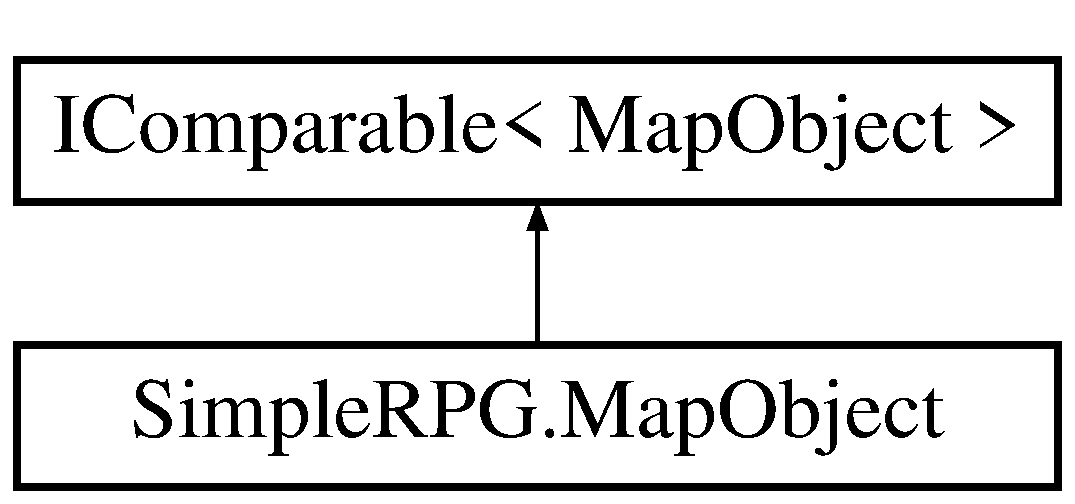
\includegraphics[height=2.000000cm]{class_simple_r_p_g_1_1_map_object}
\end{center}
\end{figure}
\subsection*{Public Member Functions}
\begin{DoxyCompactItemize}
\item 
\hypertarget{class_simple_r_p_g_1_1_map_object_ac8d60dc3cf08cb96a718209e32beecda}{{\bfseries Map\-Object} (Game game, string texture\-Name, int x\-Coord, int y\-Coord, Facing req\-Facing)}\label{class_simple_r_p_g_1_1_map_object_ac8d60dc3cf08cb96a718209e32beecda}

\item 
\hypertarget{class_simple_r_p_g_1_1_map_object_aa3fefac8f45293267c07618a32293ea0}{{\bfseries Map\-Object} (Game game, string texture\-Name, int x\-Coord, int y\-Coord)}\label{class_simple_r_p_g_1_1_map_object_aa3fefac8f45293267c07618a32293ea0}

\item 
\hypertarget{class_simple_r_p_g_1_1_map_object_a343f9c1780eb489f4bdf1539cd9c9aa0}{{\bfseries Map\-Object} (Game game, string texture\-Name, int x\-Coord, int y\-Coord, int tile\-Size)}\label{class_simple_r_p_g_1_1_map_object_a343f9c1780eb489f4bdf1539cd9c9aa0}

\item 
\hypertarget{class_simple_r_p_g_1_1_map_object_a4f44437b2648e204421cb4ebe20444b2}{void {\bfseries update} ()}\label{class_simple_r_p_g_1_1_map_object_a4f44437b2648e204421cb4ebe20444b2}

\item 
\hypertarget{class_simple_r_p_g_1_1_map_object_a1140405f31bbcc5fa466c50e0a22bb7e}{void {\bfseries draw} (Sprite\-Batch sprite\-Batch, float opacity, Point map\-Offset, int scale)}\label{class_simple_r_p_g_1_1_map_object_a1140405f31bbcc5fa466c50e0a22bb7e}

\item 
\hypertarget{class_simple_r_p_g_1_1_map_object_aee23ac75f7495b486038e13b056a6e83}{void {\bfseries move} (Point move\-Value)}\label{class_simple_r_p_g_1_1_map_object_aee23ac75f7495b486038e13b056a6e83}

\item 
\hypertarget{class_simple_r_p_g_1_1_map_object_adb50148e1809aba8d0b1c45ee5937aee}{void {\bfseries face} (Point point)}\label{class_simple_r_p_g_1_1_map_object_adb50148e1809aba8d0b1c45ee5937aee}

\item 
\hypertarget{class_simple_r_p_g_1_1_map_object_a20db9118baf359ac6b4caa6096adf097}{void {\bfseries set\-Containing\-Map} (\hyperlink{class_simple_r_p_g_1_1_tile_map}{Tile\-Map} value)}\label{class_simple_r_p_g_1_1_map_object_a20db9118baf359ac6b4caa6096adf097}

\item 
\hypertarget{class_simple_r_p_g_1_1_map_object_a2c0c5356e14e872ecc612c1c1edc4be6}{void {\bfseries set\-Passability} (\hyperlink{namespace_simple_r_p_g_a5f1ec21e7f4e36278a6cedd38c51e650}{Passability} pass)}\label{class_simple_r_p_g_1_1_map_object_a2c0c5356e14e872ecc612c1c1edc4be6}

\item 
\hypertarget{class_simple_r_p_g_1_1_map_object_aca9f243080ca6ac6d092e60d89c5b2b3}{void {\bfseries set\-Facing} (Facing face)}\label{class_simple_r_p_g_1_1_map_object_aca9f243080ca6ac6d092e60d89c5b2b3}

\item 
\hypertarget{class_simple_r_p_g_1_1_map_object_ac035cf163df3cd9b68ad0e39af9a853f}{void {\bfseries set\-Position} (int x, int y)}\label{class_simple_r_p_g_1_1_map_object_ac035cf163df3cd9b68ad0e39af9a853f}

\item 
\hypertarget{class_simple_r_p_g_1_1_map_object_a0bafe3eee08618c007b554fca627a82e}{int {\bfseries Compare\-To} (\hyperlink{class_simple_r_p_g_1_1_map_object}{Map\-Object} other)}\label{class_simple_r_p_g_1_1_map_object_a0bafe3eee08618c007b554fca627a82e}

\item 
\hypertarget{class_simple_r_p_g_1_1_map_object_a79666252fccc4b73bc87676160501a24}{\hyperlink{class_simple_r_p_g_1_1_tile_map}{Tile\-Map} {\bfseries get\-Containing\-Map} ()}\label{class_simple_r_p_g_1_1_map_object_a79666252fccc4b73bc87676160501a24}

\item 
\hypertarget{class_simple_r_p_g_1_1_map_object_ae273c60239d2162358ed06d474f6d53c}{Point {\bfseries get\-Position} ()}\label{class_simple_r_p_g_1_1_map_object_ae273c60239d2162358ed06d474f6d53c}

\item 
\hypertarget{class_simple_r_p_g_1_1_map_object_a5de0cb7af0b7060c8a842968caf4ef4e}{Point {\bfseries get\-Absolute\-Position} ()}\label{class_simple_r_p_g_1_1_map_object_a5de0cb7af0b7060c8a842968caf4ef4e}

\item 
\hypertarget{class_simple_r_p_g_1_1_map_object_a6f796cbf753b20dd31a745fb13cb6952}{Point {\bfseries get\-Offset} ()}\label{class_simple_r_p_g_1_1_map_object_a6f796cbf753b20dd31a745fb13cb6952}

\item 
\hypertarget{class_simple_r_p_g_1_1_map_object_a766ecb7691248b4af03d27a165823c2b}{int {\bfseries get\-Width} ()}\label{class_simple_r_p_g_1_1_map_object_a766ecb7691248b4af03d27a165823c2b}

\item 
\hypertarget{class_simple_r_p_g_1_1_map_object_a71210665b57a6ea94e1ad8232d067828}{int {\bfseries get\-Height} ()}\label{class_simple_r_p_g_1_1_map_object_a71210665b57a6ea94e1ad8232d067828}

\item 
\hypertarget{class_simple_r_p_g_1_1_map_object_a0c72f383828177a237a1347ce151a5ae}{\hyperlink{namespace_simple_r_p_g_a5f1ec21e7f4e36278a6cedd38c51e650}{Passability} {\bfseries get\-Passability} ()}\label{class_simple_r_p_g_1_1_map_object_a0c72f383828177a237a1347ce151a5ae}

\item 
\hypertarget{class_simple_r_p_g_1_1_map_object_a318f3ee4c39a9a5cc6fb5933c9c3778e}{bool {\bfseries is\-On\-Map} (\hyperlink{class_simple_r_p_g_1_1_tile_map}{Tile\-Map} map)}\label{class_simple_r_p_g_1_1_map_object_a318f3ee4c39a9a5cc6fb5933c9c3778e}

\end{DoxyCompactItemize}
\subsection*{Static Public Member Functions}
\begin{DoxyCompactItemize}
\item 
\hypertarget{class_simple_r_p_g_1_1_map_object_a52ee46b1a27838426c06d1324bcfde4e}{static Point {\bfseries facing\-To\-Point} (Facing face)}\label{class_simple_r_p_g_1_1_map_object_a52ee46b1a27838426c06d1324bcfde4e}

\item 
\hypertarget{class_simple_r_p_g_1_1_map_object_a4acb120e4b9fe431e0ad6f0ecb4ffb91}{static Facing {\bfseries point\-To\-Facing} (Point point)}\label{class_simple_r_p_g_1_1_map_object_a4acb120e4b9fe431e0ad6f0ecb4ffb91}

\item 
\hypertarget{class_simple_r_p_g_1_1_map_object_a213905eca91fb7aa102754c09bbb5d4b}{static int {\bfseries facing\-To\-Int} (Facing face)}\label{class_simple_r_p_g_1_1_map_object_a213905eca91fb7aa102754c09bbb5d4b}

\end{DoxyCompactItemize}
\subsection*{Protected Attributes}
\begin{DoxyCompactItemize}
\item 
\hypertarget{class_simple_r_p_g_1_1_map_object_ae014494246731c8ab9dc257ce4f2014f}{int {\bfseries id}}\label{class_simple_r_p_g_1_1_map_object_ae014494246731c8ab9dc257ce4f2014f}

\item 
\hypertarget{class_simple_r_p_g_1_1_map_object_abadd8bb893f7105e5d58914377da004b}{Point {\bfseries location}}\label{class_simple_r_p_g_1_1_map_object_abadd8bb893f7105e5d58914377da004b}

\item 
\hypertarget{class_simple_r_p_g_1_1_map_object_a74de510fc5519cc030fbd40278b3055b}{Texture2\-D {\bfseries spritesheet}}\label{class_simple_r_p_g_1_1_map_object_a74de510fc5519cc030fbd40278b3055b}

\item 
\hypertarget{class_simple_r_p_g_1_1_map_object_af2cc5123349a39665908ae723499dc89}{int {\bfseries frame}}\label{class_simple_r_p_g_1_1_map_object_af2cc5123349a39665908ae723499dc89}

\item 
\hypertarget{class_simple_r_p_g_1_1_map_object_a2f5dd4ec31a9caa81a54f7897ebbc4c7}{int {\bfseries game\-Frames\-Per\-Frame} = 3}\label{class_simple_r_p_g_1_1_map_object_a2f5dd4ec31a9caa81a54f7897ebbc4c7}

\item 
\hypertarget{class_simple_r_p_g_1_1_map_object_a8400e2878a7be96b986b3cb9c4540e25}{int {\bfseries frames\-Since\-Animation} = 0}\label{class_simple_r_p_g_1_1_map_object_a8400e2878a7be96b986b3cb9c4540e25}

\item 
\hypertarget{class_simple_r_p_g_1_1_map_object_acd8ae5f5cec25d5d2c5b8007204f2f2f}{Facing {\bfseries facing}}\label{class_simple_r_p_g_1_1_map_object_acd8ae5f5cec25d5d2c5b8007204f2f2f}

\item 
\hypertarget{class_simple_r_p_g_1_1_map_object_a80ed5dceff7ef41541cd975a55a52b01}{\hyperlink{class_simple_r_p_g_1_1_tile_map}{Tile\-Map} {\bfseries containing\-Map}}\label{class_simple_r_p_g_1_1_map_object_a80ed5dceff7ef41541cd975a55a52b01}

\item 
\hypertarget{class_simple_r_p_g_1_1_map_object_a96cebab1a15feda253342be768c52343}{bool {\bfseries moving} = false}\label{class_simple_r_p_g_1_1_map_object_a96cebab1a15feda253342be768c52343}

\item 
\hypertarget{class_simple_r_p_g_1_1_map_object_aa03f7e7baaec7a1076771ceed3d4ae70}{\hyperlink{namespace_simple_r_p_g_a5f1ec21e7f4e36278a6cedd38c51e650}{Passability} {\bfseries passability}}\label{class_simple_r_p_g_1_1_map_object_aa03f7e7baaec7a1076771ceed3d4ae70}

\end{DoxyCompactItemize}


The documentation for this class was generated from the following file\-:\begin{DoxyCompactItemize}
\item 
Simple\-R\-P\-G/\-Simple\-R\-P\-G/Map\-Object.\-cs\end{DoxyCompactItemize}

\hypertarget{class_simple_r_p_g_1_1_states_1_1_map_state}{\section{Simple\+R\+P\+G.\+States.\+Map\+State Class Reference}
\label{class_simple_r_p_g_1_1_states_1_1_map_state}\index{Simple\+R\+P\+G.\+States.\+Map\+State@{Simple\+R\+P\+G.\+States.\+Map\+State}}
}
Inheritance diagram for Simple\+R\+P\+G.\+States.\+Map\+State\+:\begin{figure}[H]
\begin{center}
\leavevmode
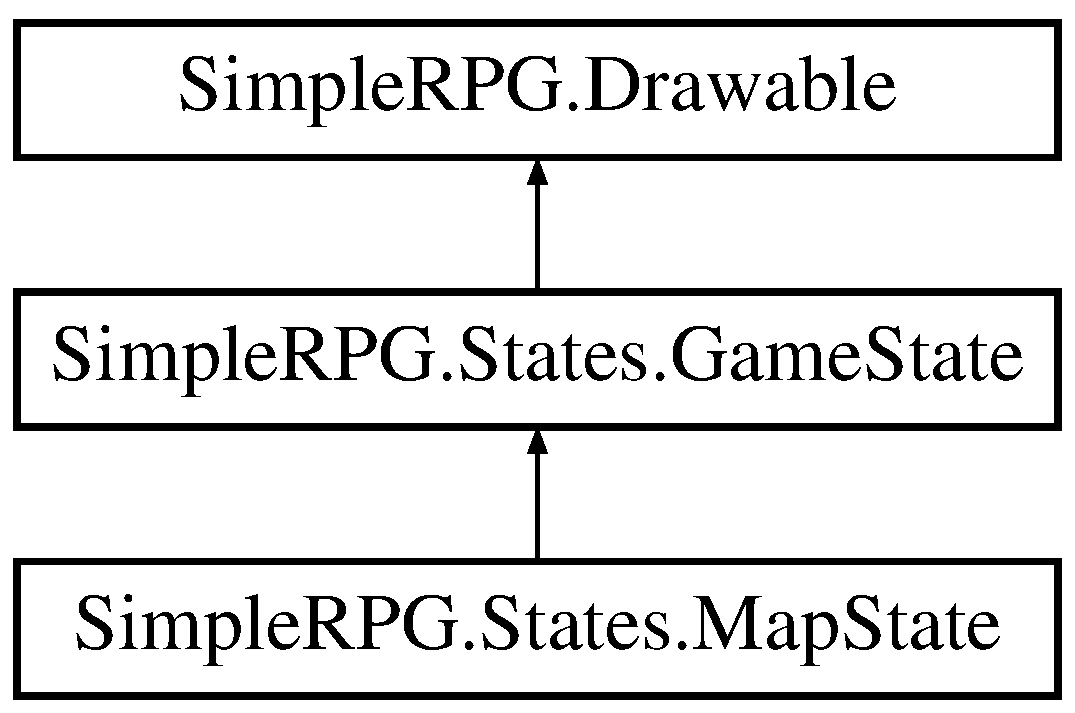
\includegraphics[height=3.000000cm]{class_simple_r_p_g_1_1_states_1_1_map_state}
\end{center}
\end{figure}
\subsection*{Public Member Functions}
\begin{DoxyCompactItemize}
\item 
\hypertarget{class_simple_r_p_g_1_1_states_1_1_map_state_a50fdccce55137f029299c1f503bc7036}{{\bfseries Map\+State} (\hyperlink{class_simple_r_p_g_1_1_game1}{Game1} game, \hyperlink{class_simple_r_p_g_1_1_states_1_1_game_state}{Game\+State} parent, \hyperlink{class_simple_r_p_g_1_1_states_1_1_state_manager}{State\+Manager} manager, \hyperlink{class_simple_r_p_g_1_1_tile_map}{Tile\+Map} req\+Map, \hyperlink{class_simple_r_p_g_1_1_camera}{Camera} req\+Camera, \hyperlink{class_simple_r_p_g_1_1_map_object}{Map\+Object} player\+Ref)}\label{class_simple_r_p_g_1_1_states_1_1_map_state_a50fdccce55137f029299c1f503bc7036}

\item 
\hypertarget{class_simple_r_p_g_1_1_states_1_1_map_state_a33046184ea7cbf635fa2523705c1b2fb}{override void {\bfseries update} ()}\label{class_simple_r_p_g_1_1_states_1_1_map_state_a33046184ea7cbf635fa2523705c1b2fb}

\item 
\hypertarget{class_simple_r_p_g_1_1_states_1_1_map_state_ad50aff095077e679434d708abb11e716}{override void {\bfseries draw} (Sprite\+Batch sprite\+Batch)}\label{class_simple_r_p_g_1_1_states_1_1_map_state_ad50aff095077e679434d708abb11e716}

\end{DoxyCompactItemize}
\subsection*{Protected Attributes}
\begin{DoxyCompactItemize}
\item 
\hypertarget{class_simple_r_p_g_1_1_states_1_1_map_state_a39f94c5063719b3a3f7657e8ed17fed6}{\hyperlink{class_simple_r_p_g_1_1_tile_map}{Tile\+Map} {\bfseries map}}\label{class_simple_r_p_g_1_1_states_1_1_map_state_a39f94c5063719b3a3f7657e8ed17fed6}

\item 
\hypertarget{class_simple_r_p_g_1_1_states_1_1_map_state_a8b39dc14b2f3e3c3b8120bf31ec79b74}{\hyperlink{class_simple_r_p_g_1_1_camera}{Camera} {\bfseries camera}}\label{class_simple_r_p_g_1_1_states_1_1_map_state_a8b39dc14b2f3e3c3b8120bf31ec79b74}

\item 
\hypertarget{class_simple_r_p_g_1_1_states_1_1_map_state_a106c108b36c278592bd8b2a660b40949}{\hyperlink{class_simple_r_p_g_1_1_map_object}{Map\+Object} {\bfseries player}}\label{class_simple_r_p_g_1_1_states_1_1_map_state_a106c108b36c278592bd8b2a660b40949}

\end{DoxyCompactItemize}
\subsection*{Additional Inherited Members}


The documentation for this class was generated from the following file\+:\begin{DoxyCompactItemize}
\item 
D\+:/\+Dropbox/\+Simple\+R\+P\+G/\+Simple\+R\+P\+G/\+Simple\+R\+P\+G/\+States/Map\+State.\+cs\end{DoxyCompactItemize}

\hypertarget{class_simple_r_p_g_1_1_events_1_1_message_event}{\section{Simple\+R\+P\+G.\+Events.\+Message\+Event Class Reference}
\label{class_simple_r_p_g_1_1_events_1_1_message_event}\index{Simple\+R\+P\+G.\+Events.\+Message\+Event@{Simple\+R\+P\+G.\+Events.\+Message\+Event}}
}
Inheritance diagram for Simple\+R\+P\+G.\+Events.\+Message\+Event\+:\begin{figure}[H]
\begin{center}
\leavevmode
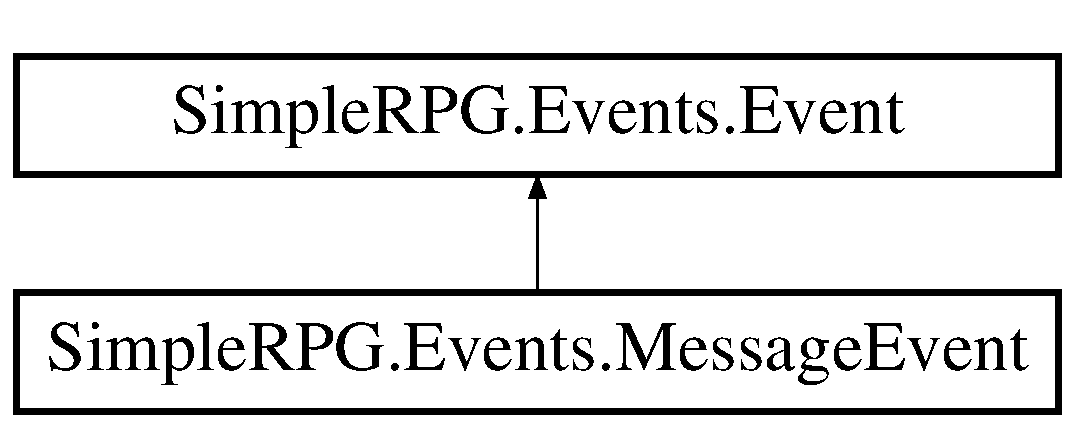
\includegraphics[height=2.000000cm]{class_simple_r_p_g_1_1_events_1_1_message_event}
\end{center}
\end{figure}
\subsection*{Public Member Functions}
\begin{DoxyCompactItemize}
\item 
\hypertarget{class_simple_r_p_g_1_1_events_1_1_message_event_ac726b325c3a3524d04eb0ec26613fe0f}{{\bfseries Message\+Event} (\hyperlink{class_simple_r_p_g_1_1_game1}{Game1} game, \hyperlink{class_simple_r_p_g_1_1_states_1_1_state_manager}{State\+Manager} manager, string req\+Message)}\label{class_simple_r_p_g_1_1_events_1_1_message_event_ac726b325c3a3524d04eb0ec26613fe0f}

\item 
\hypertarget{class_simple_r_p_g_1_1_events_1_1_message_event_ab615ebfc5d3227ecf36ca235e532a498}{override void {\bfseries start} ()}\label{class_simple_r_p_g_1_1_events_1_1_message_event_ab615ebfc5d3227ecf36ca235e532a498}

\end{DoxyCompactItemize}
\subsection*{Protected Attributes}
\begin{DoxyCompactItemize}
\item 
\hypertarget{class_simple_r_p_g_1_1_events_1_1_message_event_a0f7824800c128e02c3b41c641adc5d59}{string {\bfseries message}}\label{class_simple_r_p_g_1_1_events_1_1_message_event_a0f7824800c128e02c3b41c641adc5d59}

\end{DoxyCompactItemize}


The documentation for this class was generated from the following file\+:\begin{DoxyCompactItemize}
\item 
D\+:/\+Dropbox/\+Simple\+R\+P\+G/\+Simple\+R\+P\+G/\+Simple\+R\+P\+G/\+Events/Message\+Event.\+cs\end{DoxyCompactItemize}

\hypertarget{class_simple_r_p_g_1_1_states_1_1_message_state}{\section{Simple\-R\-P\-G.\-States.\-Message\-State Class Reference}
\label{class_simple_r_p_g_1_1_states_1_1_message_state}\index{Simple\-R\-P\-G.\-States.\-Message\-State@{Simple\-R\-P\-G.\-States.\-Message\-State}}
}
Inheritance diagram for Simple\-R\-P\-G.\-States.\-Message\-State\-:\begin{figure}[H]
\begin{center}
\leavevmode
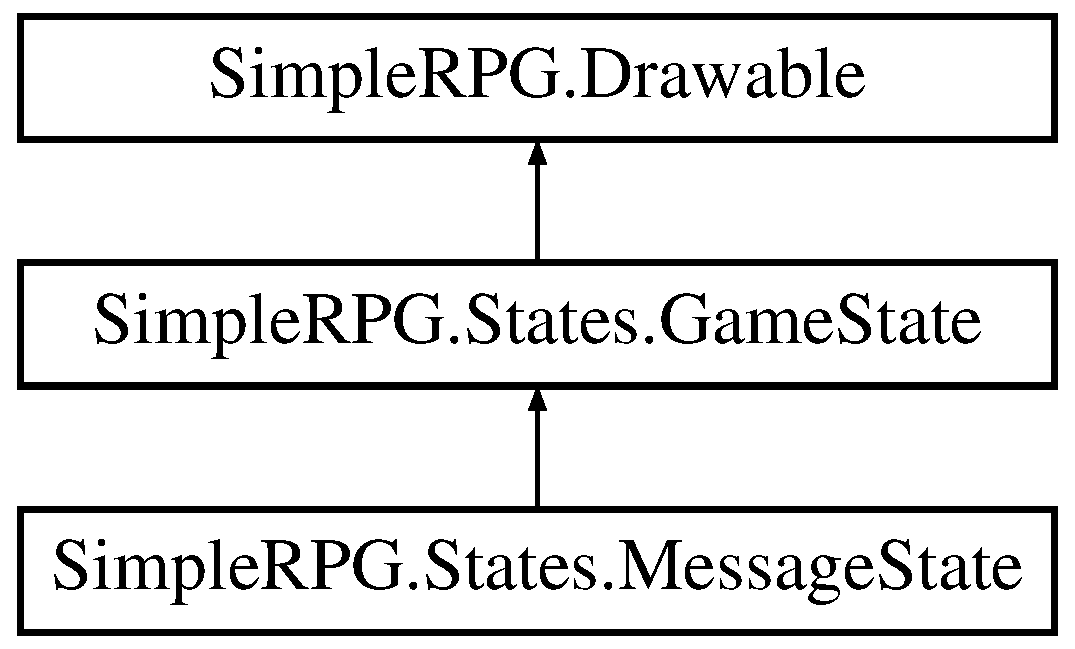
\includegraphics[height=3.000000cm]{class_simple_r_p_g_1_1_states_1_1_message_state}
\end{center}
\end{figure}
\subsection*{Public Member Functions}
\begin{DoxyCompactItemize}
\item 
\hypertarget{class_simple_r_p_g_1_1_states_1_1_message_state_a34cf4aff1d373a0dfb3a3fb663396fab}{{\bfseries Message\-State} (\hyperlink{class_simple_r_p_g_1_1_game1}{Game1} game, \hyperlink{class_simple_r_p_g_1_1_states_1_1_game_state}{Game\-State} parent, \hyperlink{class_simple_r_p_g_1_1_states_1_1_state_manager}{State\-Manager} manager, string message)}\label{class_simple_r_p_g_1_1_states_1_1_message_state_a34cf4aff1d373a0dfb3a3fb663396fab}

\item 
\hypertarget{class_simple_r_p_g_1_1_states_1_1_message_state_a400422f08ad5f53cf408e861695a3648}{override void {\bfseries update} ()}\label{class_simple_r_p_g_1_1_states_1_1_message_state_a400422f08ad5f53cf408e861695a3648}

\item 
\hypertarget{class_simple_r_p_g_1_1_states_1_1_message_state_ae1a03eead4c1e591e8d26c99dff899b9}{override void {\bfseries draw} (Sprite\-Batch sprite\-Batch)}\label{class_simple_r_p_g_1_1_states_1_1_message_state_ae1a03eead4c1e591e8d26c99dff899b9}

\end{DoxyCompactItemize}
\subsection*{Protected Attributes}
\begin{DoxyCompactItemize}
\item 
\hypertarget{class_simple_r_p_g_1_1_states_1_1_message_state_ae73420c7b3446e1db21cf6bb14861358}{\hyperlink{class_simple_r_p_g_1_1_windows_1_1_message_window}{Message\-Window} {\bfseries window}}\label{class_simple_r_p_g_1_1_states_1_1_message_state_ae73420c7b3446e1db21cf6bb14861358}

\end{DoxyCompactItemize}


The documentation for this class was generated from the following file\-:\begin{DoxyCompactItemize}
\item 
Simple\-R\-P\-G/\-Simple\-R\-P\-G/\-States/Message\-State.\-cs\end{DoxyCompactItemize}

\hypertarget{class_simple_r_p_g_1_1_windows_1_1_message_window}{\section{Simple\+R\+P\+G.\+Windows.\+Message\+Window Class Reference}
\label{class_simple_r_p_g_1_1_windows_1_1_message_window}\index{Simple\+R\+P\+G.\+Windows.\+Message\+Window@{Simple\+R\+P\+G.\+Windows.\+Message\+Window}}
}
Inheritance diagram for Simple\+R\+P\+G.\+Windows.\+Message\+Window\+:\begin{figure}[H]
\begin{center}
\leavevmode
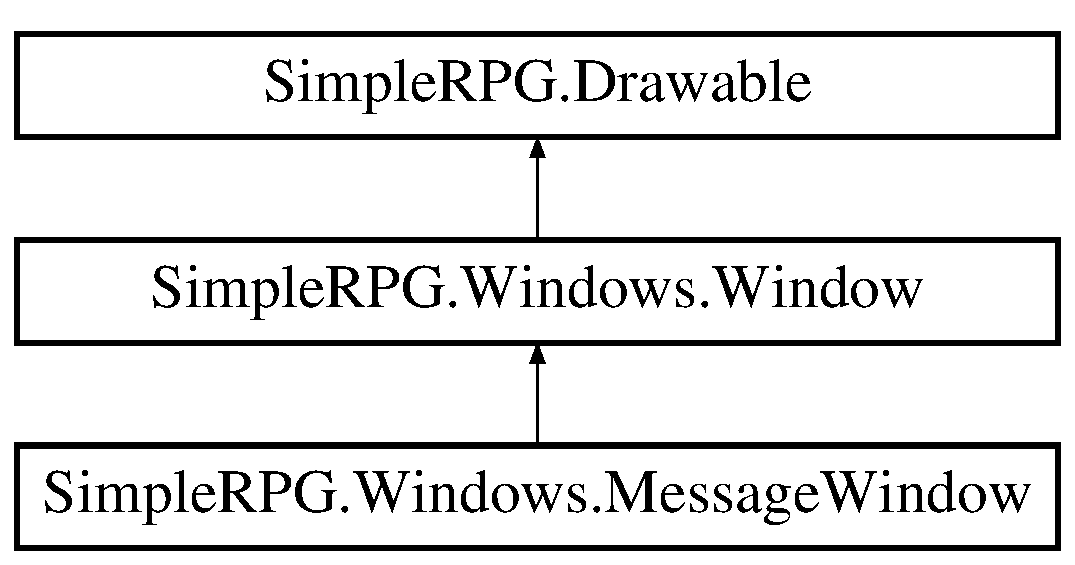
\includegraphics[height=3.000000cm]{class_simple_r_p_g_1_1_windows_1_1_message_window}
\end{center}
\end{figure}
\subsection*{Public Member Functions}
\begin{DoxyCompactItemize}
\item 
\hypertarget{class_simple_r_p_g_1_1_windows_1_1_message_window_aa0d4dc6a22265a7cc941da3891c7e7b3}{{\bfseries Message\+Window} (\hyperlink{class_simple_r_p_g_1_1_game1}{Game1} game, string req\+Message)}\label{class_simple_r_p_g_1_1_windows_1_1_message_window_aa0d4dc6a22265a7cc941da3891c7e7b3}

\item 
\hypertarget{class_simple_r_p_g_1_1_windows_1_1_message_window_aa695ec14b2b596a465dc7b5c9019298a}{override void {\bfseries update} ()}\label{class_simple_r_p_g_1_1_windows_1_1_message_window_aa695ec14b2b596a465dc7b5c9019298a}

\item 
\hypertarget{class_simple_r_p_g_1_1_windows_1_1_message_window_a1ad20623ea7ad20479a064f6b125a90b}{bool {\bfseries is\+Finished} ()}\label{class_simple_r_p_g_1_1_windows_1_1_message_window_a1ad20623ea7ad20479a064f6b125a90b}

\item 
\hypertarget{class_simple_r_p_g_1_1_windows_1_1_message_window_ad84de4bd052fa5fdede8cdb5c749dd9f}{override void {\bfseries draw} (Sprite\+Batch sprite\+Batch)}\label{class_simple_r_p_g_1_1_windows_1_1_message_window_ad84de4bd052fa5fdede8cdb5c749dd9f}

\end{DoxyCompactItemize}
\subsection*{Protected Attributes}
\begin{DoxyCompactItemize}
\item 
\hypertarget{class_simple_r_p_g_1_1_windows_1_1_message_window_a69bd0d73bf3f010d325f9162e59331be}{string {\bfseries message}}\label{class_simple_r_p_g_1_1_windows_1_1_message_window_a69bd0d73bf3f010d325f9162e59331be}

\item 
\hypertarget{class_simple_r_p_g_1_1_windows_1_1_message_window_a90d77890d714f454bb14a131e409821a}{int {\bfseries message\+Length}}\label{class_simple_r_p_g_1_1_windows_1_1_message_window_a90d77890d714f454bb14a131e409821a}

\item 
\hypertarget{class_simple_r_p_g_1_1_windows_1_1_message_window_aeaf30e10ea84c29970d99d2162439050}{Boolean {\bfseries remove\+Me} = false}\label{class_simple_r_p_g_1_1_windows_1_1_message_window_aeaf30e10ea84c29970d99d2162439050}

\end{DoxyCompactItemize}


The documentation for this class was generated from the following file\+:\begin{DoxyCompactItemize}
\item 
D\+:/\+Dropbox/\+Simple\+R\+P\+G/\+Simple\+R\+P\+G/\+Simple\+R\+P\+G/\+Windows/Message\+Window.\+cs\end{DoxyCompactItemize}

\hypertarget{class_simple_r_p_g_1_1_object_layer}{\section{Simple\-R\-P\-G.\-Object\-Layer Class Reference}
\label{class_simple_r_p_g_1_1_object_layer}\index{Simple\-R\-P\-G.\-Object\-Layer@{Simple\-R\-P\-G.\-Object\-Layer}}
}
Inheritance diagram for Simple\-R\-P\-G.\-Object\-Layer\-:\begin{figure}[H]
\begin{center}
\leavevmode
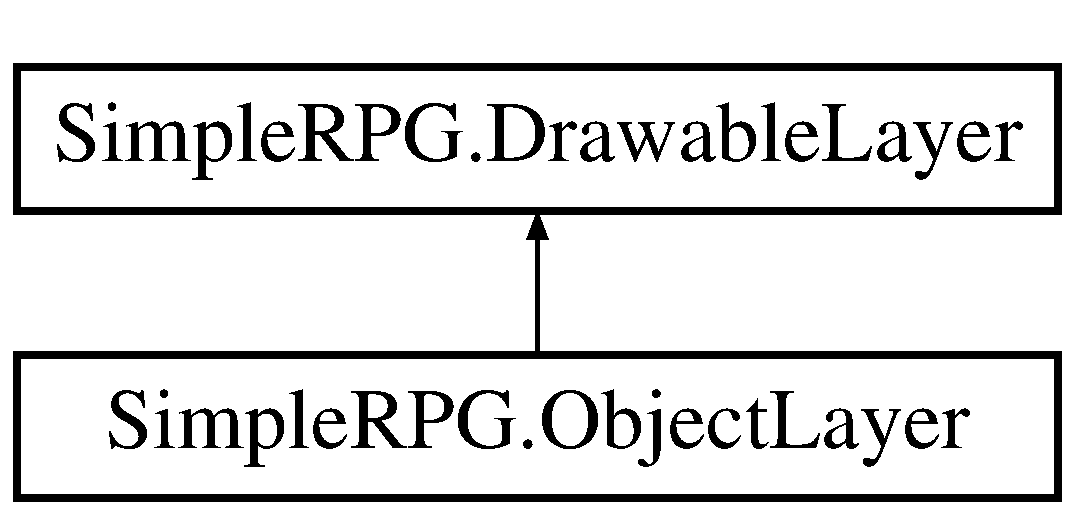
\includegraphics[height=2.000000cm]{class_simple_r_p_g_1_1_object_layer}
\end{center}
\end{figure}
\subsection*{Public Member Functions}
\begin{DoxyCompactItemize}
\item 
\hypertarget{class_simple_r_p_g_1_1_object_layer_a6f3e721aca78266fe74c2a0f3000645f}{{\bfseries Object\-Layer} (string req\-Name)}\label{class_simple_r_p_g_1_1_object_layer_a6f3e721aca78266fe74c2a0f3000645f}

\item 
\hypertarget{class_simple_r_p_g_1_1_object_layer_a799b067c1d7a5583cde3428a40c71ef2}{void {\bfseries add\-Object} (\hyperlink{class_simple_r_p_g_1_1_map_object}{Map\-Object} to\-Add)}\label{class_simple_r_p_g_1_1_object_layer_a799b067c1d7a5583cde3428a40c71ef2}

\item 
\hypertarget{class_simple_r_p_g_1_1_object_layer_acf7fff277839bac25f55a309925ed264}{void {\bfseries remove\-Object} (\hyperlink{class_simple_r_p_g_1_1_map_object}{Map\-Object} to\-Remove)}\label{class_simple_r_p_g_1_1_object_layer_acf7fff277839bac25f55a309925ed264}

\item 
\hypertarget{class_simple_r_p_g_1_1_object_layer_a1a74a83f0e799b85c0af1368dd26bc33}{override void {\bfseries update} ()}\label{class_simple_r_p_g_1_1_object_layer_a1a74a83f0e799b85c0af1368dd26bc33}

\item 
\hypertarget{class_simple_r_p_g_1_1_object_layer_a5c41bac76d7907dbcad3eb637bb74803}{override void {\bfseries draw} (Sprite\-Batch sprite\-Batch, Point first\-Tile, int tiles\-Across, int tiles\-Down, Point offset, int scale)}\label{class_simple_r_p_g_1_1_object_layer_a5c41bac76d7907dbcad3eb637bb74803}

\item 
\hypertarget{class_simple_r_p_g_1_1_object_layer_a9d519d9760d0be2acba494db6c60992d}{override \hyperlink{namespace_simple_r_p_g_a5f1ec21e7f4e36278a6cedd38c51e650}{Passability} {\bfseries get\-Passability} (int x, int y)}\label{class_simple_r_p_g_1_1_object_layer_a9d519d9760d0be2acba494db6c60992d}

\end{DoxyCompactItemize}
\subsection*{Additional Inherited Members}


The documentation for this class was generated from the following file\-:\begin{DoxyCompactItemize}
\item 
Simple\-R\-P\-G/\-Simple\-R\-P\-G/Object\-Layer.\-cs\end{DoxyCompactItemize}

\hypertarget{class_simple_r_p_g_1_1_states_1_1_pause_state}{\section{Simple\-R\-P\-G.\-States.\-Pause\-State Class Reference}
\label{class_simple_r_p_g_1_1_states_1_1_pause_state}\index{Simple\-R\-P\-G.\-States.\-Pause\-State@{Simple\-R\-P\-G.\-States.\-Pause\-State}}
}
Inheritance diagram for Simple\-R\-P\-G.\-States.\-Pause\-State\-:\begin{figure}[H]
\begin{center}
\leavevmode
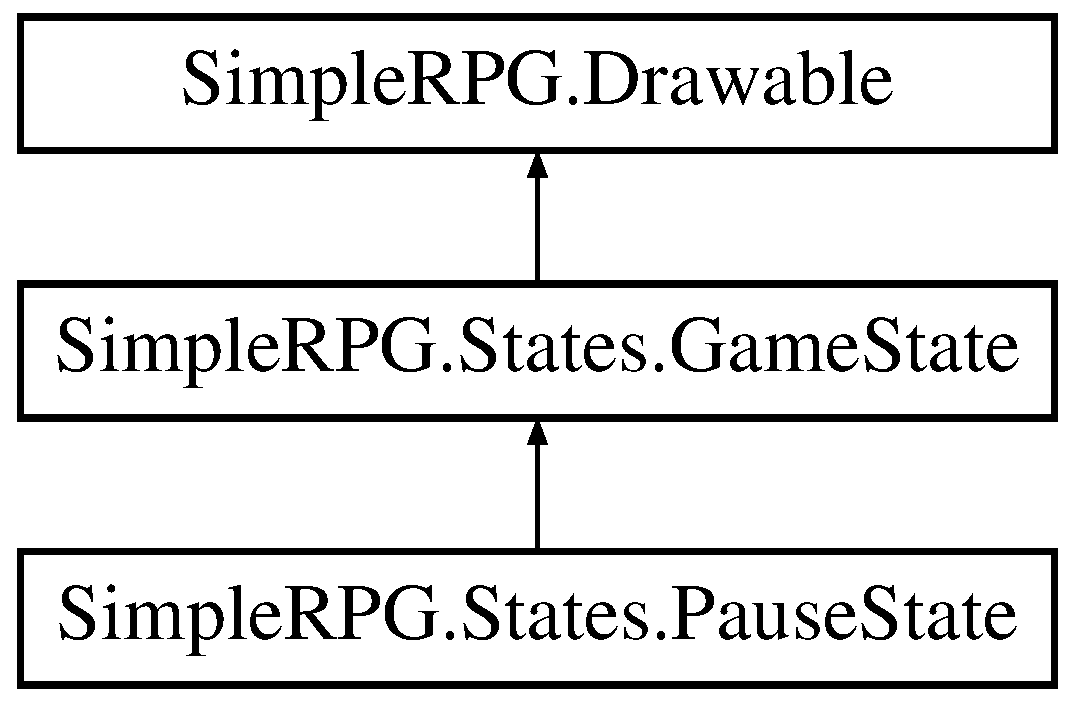
\includegraphics[height=3.000000cm]{class_simple_r_p_g_1_1_states_1_1_pause_state}
\end{center}
\end{figure}
\subsection*{Public Member Functions}
\begin{DoxyCompactItemize}
\item 
\hypertarget{class_simple_r_p_g_1_1_states_1_1_pause_state_a70f5183636726b5ec49cfc05636083a6}{{\bfseries Pause\-State} (\hyperlink{class_simple_r_p_g_1_1_game1}{Game1} game, \hyperlink{class_simple_r_p_g_1_1_states_1_1_game_state}{Game\-State} parent, \hyperlink{class_simple_r_p_g_1_1_states_1_1_state_manager}{State\-Manager} manager)}\label{class_simple_r_p_g_1_1_states_1_1_pause_state_a70f5183636726b5ec49cfc05636083a6}

\item 
\hypertarget{class_simple_r_p_g_1_1_states_1_1_pause_state_a3c042a639731a387501b22ec6f5cbd41}{override void {\bfseries update} ()}\label{class_simple_r_p_g_1_1_states_1_1_pause_state_a3c042a639731a387501b22ec6f5cbd41}

\item 
\hypertarget{class_simple_r_p_g_1_1_states_1_1_pause_state_aa364801aece7b7497a0f09fe3fc41085}{override void {\bfseries draw} (Sprite\-Batch sprite\-Batch)}\label{class_simple_r_p_g_1_1_states_1_1_pause_state_aa364801aece7b7497a0f09fe3fc41085}

\end{DoxyCompactItemize}
\subsection*{Protected Attributes}
\begin{DoxyCompactItemize}
\item 
\hypertarget{class_simple_r_p_g_1_1_states_1_1_pause_state_a5ca649a458e41330e32f5f4cc68fc66e}{\hyperlink{class_simple_r_p_g_1_1_windows_1_1_list_box}{List\-Box} {\bfseries pause\-Window}}\label{class_simple_r_p_g_1_1_states_1_1_pause_state_a5ca649a458e41330e32f5f4cc68fc66e}

\end{DoxyCompactItemize}


The documentation for this class was generated from the following file\-:\begin{DoxyCompactItemize}
\item 
Simple\-R\-P\-G/\-Simple\-R\-P\-G/\-States/Pause\-State.\-cs\end{DoxyCompactItemize}

\hypertarget{class_simple_r_p_g_1_1_windows_1_1_pause_window}{\section{Simple\+R\+P\+G.\+Windows.\+Pause\+Window Class Reference}
\label{class_simple_r_p_g_1_1_windows_1_1_pause_window}\index{Simple\+R\+P\+G.\+Windows.\+Pause\+Window@{Simple\+R\+P\+G.\+Windows.\+Pause\+Window}}
}
Inheritance diagram for Simple\+R\+P\+G.\+Windows.\+Pause\+Window\+:\begin{figure}[H]
\begin{center}
\leavevmode
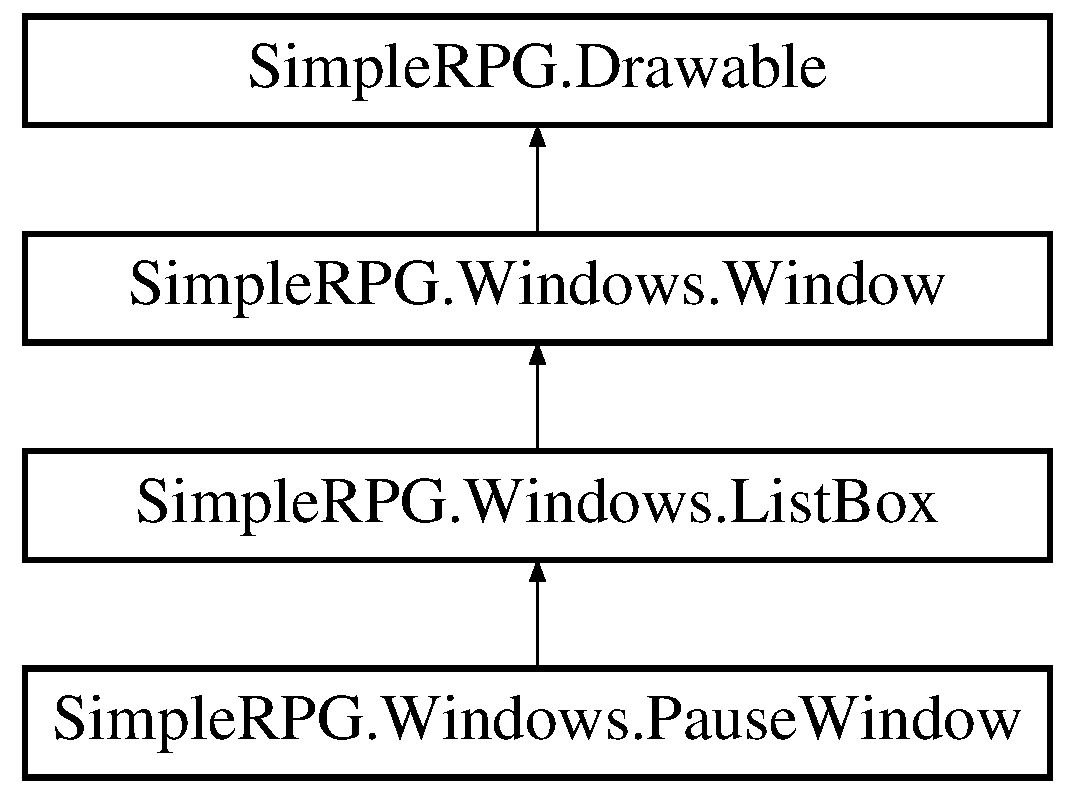
\includegraphics[height=4.000000cm]{class_simple_r_p_g_1_1_windows_1_1_pause_window}
\end{center}
\end{figure}
\subsection*{Public Member Functions}
\begin{DoxyCompactItemize}
\item 
\hypertarget{class_simple_r_p_g_1_1_windows_1_1_pause_window_a70df9c6ba9111340a7ef0dd7ecd09ab6}{{\bfseries Pause\+Window} (\hyperlink{class_simple_r_p_g_1_1_game1}{Game1} game)}\label{class_simple_r_p_g_1_1_windows_1_1_pause_window_a70df9c6ba9111340a7ef0dd7ecd09ab6}

\end{DoxyCompactItemize}
\subsection*{Additional Inherited Members}


The documentation for this class was generated from the following file\+:\begin{DoxyCompactItemize}
\item 
D\+:/\+Dropbox/\+Simple\+R\+P\+G/\+Simple\+R\+P\+G/\+Simple\+R\+P\+G/\+Windows/Pause\+Window.\+cs\end{DoxyCompactItemize}

\hypertarget{class_simple_r_p_g_1_1_player}{\section{Simple\+R\+P\+G.\+Player Class Reference}
\label{class_simple_r_p_g_1_1_player}\index{Simple\+R\+P\+G.\+Player@{Simple\+R\+P\+G.\+Player}}
}
\subsection*{Static Public Member Functions}
\begin{DoxyCompactItemize}
\item 
\hypertarget{class_simple_r_p_g_1_1_player_a848b6a19ab65bf51097e7e4cb47ad021}{static void {\bfseries initialize} ()}\label{class_simple_r_p_g_1_1_player_a848b6a19ab65bf51097e7e4cb47ad021}

\item 
\hypertarget{class_simple_r_p_g_1_1_player_a7b7f4514e3020e56a948316ef1fb5cc9}{static \hyperlink{class_simple_r_p_g_1_1_item_container}{Item\+Container} {\bfseries get\+Inventory} ()}\label{class_simple_r_p_g_1_1_player_a7b7f4514e3020e56a948316ef1fb5cc9}

\item 
\hypertarget{class_simple_r_p_g_1_1_player_ab5267292b513dc9b853f607dd34b1c38}{static void {\bfseries give\+Item} (\hyperlink{class_simple_r_p_g_1_1_item}{Item} item)}\label{class_simple_r_p_g_1_1_player_ab5267292b513dc9b853f607dd34b1c38}

\item 
\hypertarget{class_simple_r_p_g_1_1_player_a50294b9cd7ca33f530dce63e83b0acfe}{static void {\bfseries take\+Item} (\hyperlink{class_simple_r_p_g_1_1_item}{Item} item)}\label{class_simple_r_p_g_1_1_player_a50294b9cd7ca33f530dce63e83b0acfe}

\item 
\hypertarget{class_simple_r_p_g_1_1_player_a94a62653441c455e38a9572ccc6b8936}{static List$<$ \hyperlink{class_simple_r_p_g_1_1_battler}{Battler} $>$ {\bfseries get\+Party} ()}\label{class_simple_r_p_g_1_1_player_a94a62653441c455e38a9572ccc6b8936}

\end{DoxyCompactItemize}
\subsection*{Static Protected Attributes}
\begin{DoxyCompactItemize}
\item 
\hypertarget{class_simple_r_p_g_1_1_player_a64192a3f860c47d7a67fc885dbb8ffcd}{static \hyperlink{class_simple_r_p_g_1_1_item_container}{Item\+Container} {\bfseries inventory} = new \hyperlink{class_simple_r_p_g_1_1_item_container}{Item\+Container}()}\label{class_simple_r_p_g_1_1_player_a64192a3f860c47d7a67fc885dbb8ffcd}

\item 
\hypertarget{class_simple_r_p_g_1_1_player_a254855437c04bc8cbc74d63225b05bfe}{static List$<$ \hyperlink{class_simple_r_p_g_1_1_battler}{Battler} $>$ {\bfseries party} = new List$<$\hyperlink{class_simple_r_p_g_1_1_battler}{Battler}$>$()}\label{class_simple_r_p_g_1_1_player_a254855437c04bc8cbc74d63225b05bfe}

\end{DoxyCompactItemize}


The documentation for this class was generated from the following file\+:\begin{DoxyCompactItemize}
\item 
D\+:/\+Dropbox/\+Simple\+R\+P\+G/\+Simple\+R\+P\+G/\+Simple\+R\+P\+G/Player.\+cs\end{DoxyCompactItemize}

\hypertarget{class_simple_r_p_g_1_1_player_battler}{\section{Simple\+R\+P\+G.\+Player\+Battler Class Reference}
\label{class_simple_r_p_g_1_1_player_battler}\index{Simple\+R\+P\+G.\+Player\+Battler@{Simple\+R\+P\+G.\+Player\+Battler}}
}
Inheritance diagram for Simple\+R\+P\+G.\+Player\+Battler\+:\begin{figure}[H]
\begin{center}
\leavevmode
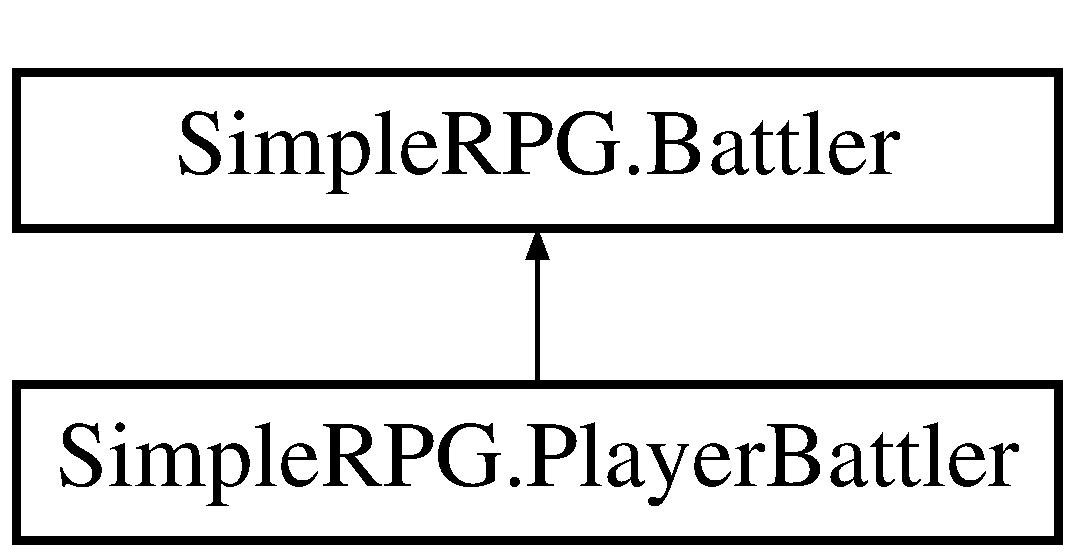
\includegraphics[height=2.000000cm]{class_simple_r_p_g_1_1_player_battler}
\end{center}
\end{figure}
\subsection*{Additional Inherited Members}


The documentation for this class was generated from the following file\+:\begin{DoxyCompactItemize}
\item 
D\+:/\+Dropbox/\+Simple\+R\+P\+G/\+Simple\+R\+P\+G/\+Simple\+R\+P\+G/Player\+Battler.\+cs\end{DoxyCompactItemize}

\hypertarget{class_simple_r_p_g_1_1_windows_1_1_player_battle_status_window}{\section{Simple\+R\+P\+G.\+Windows.\+Player\+Battle\+Status\+Window Class Reference}
\label{class_simple_r_p_g_1_1_windows_1_1_player_battle_status_window}\index{Simple\+R\+P\+G.\+Windows.\+Player\+Battle\+Status\+Window@{Simple\+R\+P\+G.\+Windows.\+Player\+Battle\+Status\+Window}}
}
Inheritance diagram for Simple\+R\+P\+G.\+Windows.\+Player\+Battle\+Status\+Window\+:\begin{figure}[H]
\begin{center}
\leavevmode
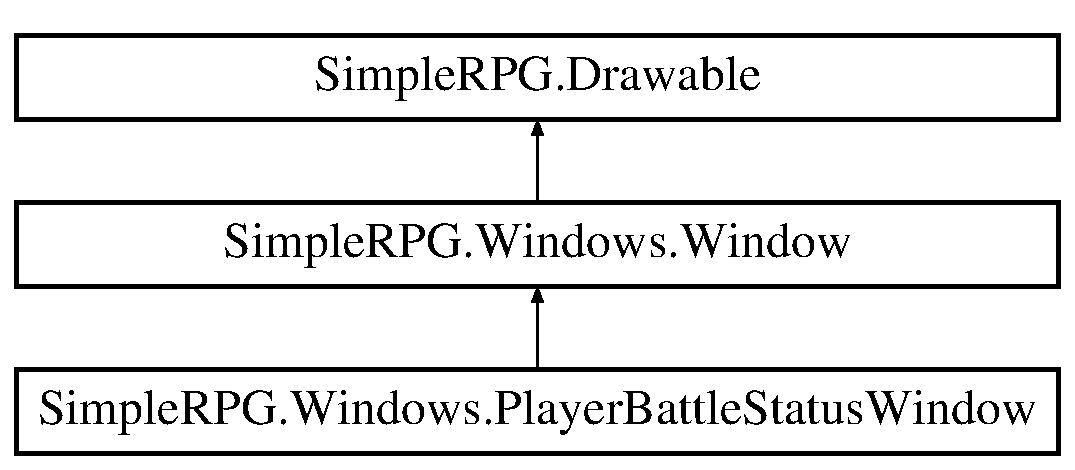
\includegraphics[height=3.000000cm]{class_simple_r_p_g_1_1_windows_1_1_player_battle_status_window}
\end{center}
\end{figure}
\subsection*{Public Member Functions}
\begin{DoxyCompactItemize}
\item 
\hypertarget{class_simple_r_p_g_1_1_windows_1_1_player_battle_status_window_ae2ad2483a7a871d0d4680c9aa232ee76}{{\bfseries Player\+Battle\+Status\+Window} (\hyperlink{class_simple_r_p_g_1_1_game1}{Game1} game, Point req\+Position, string windowskin, \hyperlink{class_simple_r_p_g_1_1_battler}{Battler} battler)}\label{class_simple_r_p_g_1_1_windows_1_1_player_battle_status_window_ae2ad2483a7a871d0d4680c9aa232ee76}

\item 
\hypertarget{class_simple_r_p_g_1_1_windows_1_1_player_battle_status_window_a24e6f06bae4c4aef79a4a935ee2536ab}{override void {\bfseries update} ()}\label{class_simple_r_p_g_1_1_windows_1_1_player_battle_status_window_a24e6f06bae4c4aef79a4a935ee2536ab}

\item 
\hypertarget{class_simple_r_p_g_1_1_windows_1_1_player_battle_status_window_abbb624620fe13be8267c0ab4ad440d95}{override void {\bfseries draw} (Sprite\+Batch sprite\+Batch)}\label{class_simple_r_p_g_1_1_windows_1_1_player_battle_status_window_abbb624620fe13be8267c0ab4ad440d95}

\end{DoxyCompactItemize}
\subsection*{Protected Attributes}
\begin{DoxyCompactItemize}
\item 
\hypertarget{class_simple_r_p_g_1_1_windows_1_1_player_battle_status_window_a3dc74bda60f07aa2648e52c9d1d0ae64}{\hyperlink{class_simple_r_p_g_1_1_battler}{Battler} {\bfseries player}}\label{class_simple_r_p_g_1_1_windows_1_1_player_battle_status_window_a3dc74bda60f07aa2648e52c9d1d0ae64}

\item 
\hypertarget{class_simple_r_p_g_1_1_windows_1_1_player_battle_status_window_a26394a47b764a11d91455d3f3212efd0}{Texture2\+D {\bfseries player\+Health}}\label{class_simple_r_p_g_1_1_windows_1_1_player_battle_status_window_a26394a47b764a11d91455d3f3212efd0}

\item 
\hypertarget{class_simple_r_p_g_1_1_windows_1_1_player_battle_status_window_a62f2437b21ed476211989db68f3e77f8}{Color {\bfseries hp\+Color} = Color.\+White}\label{class_simple_r_p_g_1_1_windows_1_1_player_battle_status_window_a62f2437b21ed476211989db68f3e77f8}

\item 
\hypertarget{class_simple_r_p_g_1_1_windows_1_1_player_battle_status_window_a07a3053b58268a4d79ee3f1f62c2a53f}{int {\bfseries hp\+Grad} = 0}\label{class_simple_r_p_g_1_1_windows_1_1_player_battle_status_window_a07a3053b58268a4d79ee3f1f62c2a53f}

\end{DoxyCompactItemize}


The documentation for this class was generated from the following file\+:\begin{DoxyCompactItemize}
\item 
D\+:/\+Dropbox/\+Simple\+R\+P\+G/\+Simple\+R\+P\+G/\+Simple\+R\+P\+G/\+Windows/Player\+Battle\+Status\+Window.\+cs\end{DoxyCompactItemize}

\hypertarget{class_simple_r_p_g_1_1_states_1_1_state_manager}{\section{Simple\-R\-P\-G.\-States.\-State\-Manager Class Reference}
\label{class_simple_r_p_g_1_1_states_1_1_state_manager}\index{Simple\-R\-P\-G.\-States.\-State\-Manager@{Simple\-R\-P\-G.\-States.\-State\-Manager}}
}
\subsection*{Public Member Functions}
\begin{DoxyCompactItemize}
\item 
\hypertarget{class_simple_r_p_g_1_1_states_1_1_state_manager_a190d4de26a1b06b94cf488a124fd407d}{{\bfseries State\-Manager} (\hyperlink{class_simple_r_p_g_1_1_game1}{Game1} game)}\label{class_simple_r_p_g_1_1_states_1_1_state_manager_a190d4de26a1b06b94cf488a124fd407d}

\item 
\hypertarget{class_simple_r_p_g_1_1_states_1_1_state_manager_ae5698b19b0cf74dec089f2217bbb7b94}{void {\bfseries add\-State} (\hyperlink{class_simple_r_p_g_1_1_states_1_1_game_state}{Game\-State} new\-State)}\label{class_simple_r_p_g_1_1_states_1_1_state_manager_ae5698b19b0cf74dec089f2217bbb7b94}

\item 
\hypertarget{class_simple_r_p_g_1_1_states_1_1_state_manager_a082635e320668aeb0b4e386c00e26b95}{\hyperlink{class_simple_r_p_g_1_1_states_1_1_game_state}{Game\-State} {\bfseries pop\-State} ()}\label{class_simple_r_p_g_1_1_states_1_1_state_manager_a082635e320668aeb0b4e386c00e26b95}

\item 
\hypertarget{class_simple_r_p_g_1_1_states_1_1_state_manager_ab2299a6b8ec00cb7954f2482e61f6d9d}{\hyperlink{class_simple_r_p_g_1_1_states_1_1_game_state}{Game\-State} {\bfseries get\-Current\-State} ()}\label{class_simple_r_p_g_1_1_states_1_1_state_manager_ab2299a6b8ec00cb7954f2482e61f6d9d}

\item 
\hypertarget{class_simple_r_p_g_1_1_states_1_1_state_manager_a8b6fc7246fed3a0b56b863289fa6afd0}{\hyperlink{class_simple_r_p_g_1_1_states_1_1_game_state}{Game\-State} {\bfseries remove\-State} (\hyperlink{class_simple_r_p_g_1_1_states_1_1_game_state}{Game\-State} state)}\label{class_simple_r_p_g_1_1_states_1_1_state_manager_a8b6fc7246fed3a0b56b863289fa6afd0}

\item 
\hypertarget{class_simple_r_p_g_1_1_states_1_1_state_manager_a087db2b322e7df7dd718fe9bfa8de005}{void {\bfseries update} ()}\label{class_simple_r_p_g_1_1_states_1_1_state_manager_a087db2b322e7df7dd718fe9bfa8de005}

\item 
\hypertarget{class_simple_r_p_g_1_1_states_1_1_state_manager_a79b249bd1e60b228ad9666b02b6308cf}{void {\bfseries draw} (Sprite\-Batch sprite\-Batch)}\label{class_simple_r_p_g_1_1_states_1_1_state_manager_a79b249bd1e60b228ad9666b02b6308cf}

\item 
\hypertarget{class_simple_r_p_g_1_1_states_1_1_state_manager_a1d346eab57b9633c88d051d555919921}{void {\bfseries clear} ()}\label{class_simple_r_p_g_1_1_states_1_1_state_manager_a1d346eab57b9633c88d051d555919921}

\item 
\hypertarget{class_simple_r_p_g_1_1_states_1_1_state_manager_a11cac71d35a247ebc836576c779f8b61}{bool {\bfseries is\-Empty} ()}\label{class_simple_r_p_g_1_1_states_1_1_state_manager_a11cac71d35a247ebc836576c779f8b61}

\end{DoxyCompactItemize}


The documentation for this class was generated from the following file\-:\begin{DoxyCompactItemize}
\item 
Simple\-R\-P\-G/\-Simple\-R\-P\-G/\-States/State\-Manager.\-cs\end{DoxyCompactItemize}

\hypertarget{class_simple_r_p_g_1_1_states_1_1_target_select_state}{\section{Simple\-R\-P\-G.\-States.\-Target\-Select\-State Class Reference}
\label{class_simple_r_p_g_1_1_states_1_1_target_select_state}\index{Simple\-R\-P\-G.\-States.\-Target\-Select\-State@{Simple\-R\-P\-G.\-States.\-Target\-Select\-State}}
}
Inheritance diagram for Simple\-R\-P\-G.\-States.\-Target\-Select\-State\-:\begin{figure}[H]
\begin{center}
\leavevmode
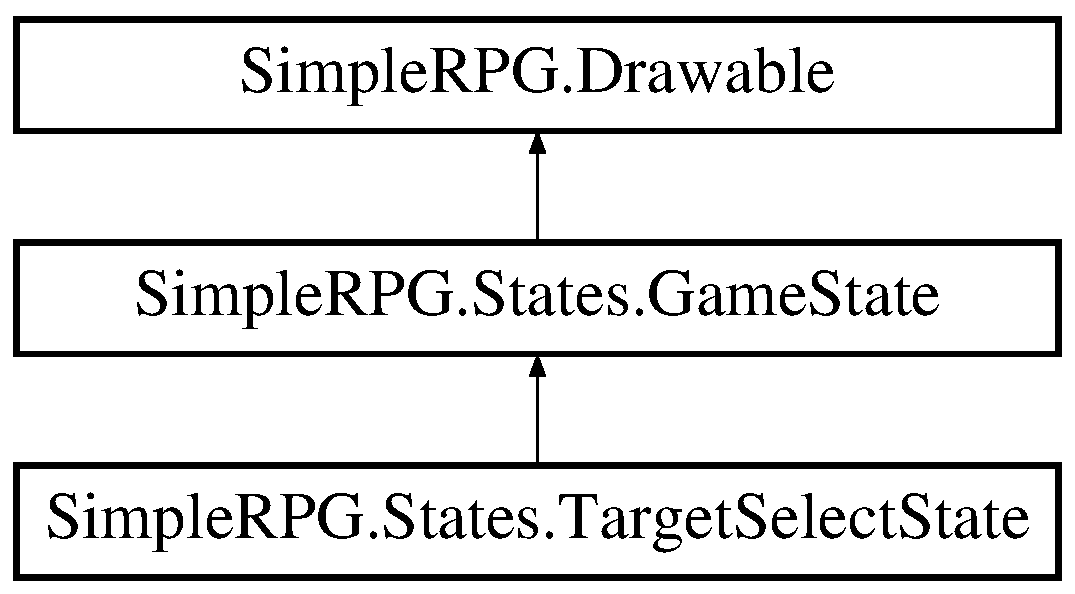
\includegraphics[height=3.000000cm]{class_simple_r_p_g_1_1_states_1_1_target_select_state}
\end{center}
\end{figure}
\subsection*{Public Member Functions}
\begin{DoxyCompactItemize}
\item 
\hypertarget{class_simple_r_p_g_1_1_states_1_1_target_select_state_abc7562e63e14f09da3ca852ff0b90435}{{\bfseries Target\-Select\-State} (\hyperlink{class_simple_r_p_g_1_1_game1}{Game1} game, \hyperlink{class_simple_r_p_g_1_1_states_1_1_game_state}{Game\-State} parent, \hyperlink{class_simple_r_p_g_1_1_states_1_1_state_manager}{State\-Manager} manager, List$<$ \hyperlink{class_simple_r_p_g_1_1_battler}{Battler} $>$ battlers)}\label{class_simple_r_p_g_1_1_states_1_1_target_select_state_abc7562e63e14f09da3ca852ff0b90435}

\item 
\hypertarget{class_simple_r_p_g_1_1_states_1_1_target_select_state_a4b729abe4fd79d8e152a2eb8af5042ea}{override void {\bfseries update} ()}\label{class_simple_r_p_g_1_1_states_1_1_target_select_state_a4b729abe4fd79d8e152a2eb8af5042ea}

\item 
\hypertarget{class_simple_r_p_g_1_1_states_1_1_target_select_state_a614028f6f0d57d1f7c7e4e0cf9e879e3}{override void {\bfseries draw} (Sprite\-Batch sprite\-Batch)}\label{class_simple_r_p_g_1_1_states_1_1_target_select_state_a614028f6f0d57d1f7c7e4e0cf9e879e3}

\end{DoxyCompactItemize}
\subsection*{Protected Attributes}
\begin{DoxyCompactItemize}
\item 
\hypertarget{class_simple_r_p_g_1_1_states_1_1_target_select_state_a83b2a454f571a185bfd77e453bc53c6f}{\hyperlink{class_simple_r_p_g_1_1_windows_1_1_list_box}{List\-Box} {\bfseries targets}}\label{class_simple_r_p_g_1_1_states_1_1_target_select_state_a83b2a454f571a185bfd77e453bc53c6f}

\item 
\hypertarget{class_simple_r_p_g_1_1_states_1_1_target_select_state_a9ecf5e51040139dddfc80fefa399fd96}{List$<$ \hyperlink{class_simple_r_p_g_1_1_battler}{Battler} $>$ {\bfseries enemies}}\label{class_simple_r_p_g_1_1_states_1_1_target_select_state_a9ecf5e51040139dddfc80fefa399fd96}

\end{DoxyCompactItemize}


The documentation for this class was generated from the following file\-:\begin{DoxyCompactItemize}
\item 
Simple\-R\-P\-G/\-Simple\-R\-P\-G/\-States/Target\-Select\-State.\-cs\end{DoxyCompactItemize}

\hypertarget{class_simple_r_p_g_1_1_widgets_1_1_text_widget}{\section{Simple\-R\-P\-G.\-Widgets.\-Text\-Widget Class Reference}
\label{class_simple_r_p_g_1_1_widgets_1_1_text_widget}\index{Simple\-R\-P\-G.\-Widgets.\-Text\-Widget@{Simple\-R\-P\-G.\-Widgets.\-Text\-Widget}}
}
Inheritance diagram for Simple\-R\-P\-G.\-Widgets.\-Text\-Widget\-:\begin{figure}[H]
\begin{center}
\leavevmode
\includegraphics[height=2.592592cm]{class_simple_r_p_g_1_1_widgets_1_1_text_widget}
\end{center}
\end{figure}
\subsection*{Public Member Functions}
\begin{DoxyCompactItemize}
\item 
\hypertarget{class_simple_r_p_g_1_1_widgets_1_1_text_widget_ae761ed26cba45dabf2fc2be7b8dba38a}{{\bfseries Text\-Widget} (Sprite\-Font req\-Font, Color req\-Color, Vector2 req\-Position)}\label{class_simple_r_p_g_1_1_widgets_1_1_text_widget_ae761ed26cba45dabf2fc2be7b8dba38a}

\item 
\hypertarget{class_simple_r_p_g_1_1_widgets_1_1_text_widget_ae9e3cb7b4fbb8b7b04f92357dbd17fe0}{{\bfseries Text\-Widget} (Sprite\-Font req\-Font, Color req\-Color, Vector2 req\-Position, string req\-Text)}\label{class_simple_r_p_g_1_1_widgets_1_1_text_widget_ae9e3cb7b4fbb8b7b04f92357dbd17fe0}

\item 
\hypertarget{class_simple_r_p_g_1_1_widgets_1_1_text_widget_ae3f13c0514cc686cb7f6da6fd2165ed2}{override void {\bfseries update} ()}\label{class_simple_r_p_g_1_1_widgets_1_1_text_widget_ae3f13c0514cc686cb7f6da6fd2165ed2}

\item 
\hypertarget{class_simple_r_p_g_1_1_widgets_1_1_text_widget_af6ceb5dc2687ec28769d4b2298518d6d}{void {\bfseries set\-Text} (string new\-Text)}\label{class_simple_r_p_g_1_1_widgets_1_1_text_widget_af6ceb5dc2687ec28769d4b2298518d6d}

\item 
\hypertarget{class_simple_r_p_g_1_1_widgets_1_1_text_widget_a99fe0ea10942a791c12a44d714a8fef1}{override void {\bfseries draw} (Sprite\-Batch sprite\-Batch)}\label{class_simple_r_p_g_1_1_widgets_1_1_text_widget_a99fe0ea10942a791c12a44d714a8fef1}

\item 
\hypertarget{class_simple_r_p_g_1_1_widgets_1_1_text_widget_ac30d0584dbcb9d0c954aa3992465b9d4}{void {\bfseries flash} (Color new\-Color)}\label{class_simple_r_p_g_1_1_widgets_1_1_text_widget_ac30d0584dbcb9d0c954aa3992465b9d4}

\item 
\hypertarget{class_simple_r_p_g_1_1_widgets_1_1_text_widget_a9cb6e2092c1f2dc616b3c64260e9d5c3}{void {\bfseries stop\-Flash} ()}\label{class_simple_r_p_g_1_1_widgets_1_1_text_widget_a9cb6e2092c1f2dc616b3c64260e9d5c3}

\item 
\hypertarget{class_simple_r_p_g_1_1_widgets_1_1_text_widget_a3e2de1a7627205b0221e009190d9f0f2}{void {\bfseries set\-Position} (Vector2 pos)}\label{class_simple_r_p_g_1_1_widgets_1_1_text_widget_a3e2de1a7627205b0221e009190d9f0f2}

\end{DoxyCompactItemize}
\subsection*{Protected Member Functions}
\begin{DoxyCompactItemize}
\item 
\hypertarget{class_simple_r_p_g_1_1_widgets_1_1_text_widget_a8d1cf29c11acc868070c897d51f0000c}{void {\bfseries flash\-Update} ()}\label{class_simple_r_p_g_1_1_widgets_1_1_text_widget_a8d1cf29c11acc868070c897d51f0000c}

\end{DoxyCompactItemize}
\subsection*{Protected Attributes}
\begin{DoxyCompactItemize}
\item 
\hypertarget{class_simple_r_p_g_1_1_widgets_1_1_text_widget_a060fc2ff5ce833c130788873116049cb}{string {\bfseries text} = \char`\"{}\char`\"{}}\label{class_simple_r_p_g_1_1_widgets_1_1_text_widget_a060fc2ff5ce833c130788873116049cb}

\item 
\hypertarget{class_simple_r_p_g_1_1_widgets_1_1_text_widget_abf9e9cf9275582afe162d971bfaf2d01}{Sprite\-Font {\bfseries font}}\label{class_simple_r_p_g_1_1_widgets_1_1_text_widget_abf9e9cf9275582afe162d971bfaf2d01}

\item 
\hypertarget{class_simple_r_p_g_1_1_widgets_1_1_text_widget_a37a150b972ba5f086821b5729af3b6f6}{Vector2 {\bfseries position}}\label{class_simple_r_p_g_1_1_widgets_1_1_text_widget_a37a150b972ba5f086821b5729af3b6f6}

\item 
\hypertarget{class_simple_r_p_g_1_1_widgets_1_1_text_widget_a221a6baebf53762f1e1f282a4febbe72}{Color {\bfseries color}}\label{class_simple_r_p_g_1_1_widgets_1_1_text_widget_a221a6baebf53762f1e1f282a4febbe72}

\item 
\hypertarget{class_simple_r_p_g_1_1_widgets_1_1_text_widget_ad8813c5ec28a1d75aaad00efdd895a2c}{Color {\bfseries flash\-Color}}\label{class_simple_r_p_g_1_1_widgets_1_1_text_widget_ad8813c5ec28a1d75aaad00efdd895a2c}

\item 
\hypertarget{class_simple_r_p_g_1_1_widgets_1_1_text_widget_a64872fa01dadc9aca4c02432407d5807}{int {\bfseries red\-Change}}\label{class_simple_r_p_g_1_1_widgets_1_1_text_widget_a64872fa01dadc9aca4c02432407d5807}

\item 
\hypertarget{class_simple_r_p_g_1_1_widgets_1_1_text_widget_a19c259ba6a56c9a7763e46160b8b0a9f}{bool {\bfseries flashing}}\label{class_simple_r_p_g_1_1_widgets_1_1_text_widget_a19c259ba6a56c9a7763e46160b8b0a9f}

\end{DoxyCompactItemize}


The documentation for this class was generated from the following file\-:\begin{DoxyCompactItemize}
\item 
Simple\-R\-P\-G/\-Simple\-R\-P\-G/\-Widgets/Text\-Widget.\-cs\end{DoxyCompactItemize}

\hypertarget{class_simple_r_p_g_1_1_tile}{\section{Simple\-R\-P\-G.\-Tile Class Reference}
\label{class_simple_r_p_g_1_1_tile}\index{Simple\-R\-P\-G.\-Tile@{Simple\-R\-P\-G.\-Tile}}
}
\subsection*{Public Member Functions}
\begin{DoxyCompactItemize}
\item 
\hypertarget{class_simple_r_p_g_1_1_tile_a069f215130a286a98934195b2202a6db}{{\bfseries Tile} (\hyperlink{namespace_simple_r_p_g_a5f1ec21e7f4e36278a6cedd38c51e650}{Passability} req\-Passability, int req\-Tile\-I\-D)}\label{class_simple_r_p_g_1_1_tile_a069f215130a286a98934195b2202a6db}

\item 
\hypertarget{class_simple_r_p_g_1_1_tile_abbdfa6a9bf0934cca5258a5ff856c2af}{\hyperlink{namespace_simple_r_p_g_a5f1ec21e7f4e36278a6cedd38c51e650}{Passability} {\bfseries get\-Passability} ()}\label{class_simple_r_p_g_1_1_tile_abbdfa6a9bf0934cca5258a5ff856c2af}

\item 
\hypertarget{class_simple_r_p_g_1_1_tile_acc379dfbc9f1aacd7c369de976fb187c}{int {\bfseries get\-Tile\-I\-D} ()}\label{class_simple_r_p_g_1_1_tile_acc379dfbc9f1aacd7c369de976fb187c}

\item 
\hypertarget{class_simple_r_p_g_1_1_tile_ad8da34417ef806406e93bb602f3f95fd}{Color {\bfseries get\-Tint} ()}\label{class_simple_r_p_g_1_1_tile_ad8da34417ef806406e93bb602f3f95fd}

\item 
\hypertarget{class_simple_r_p_g_1_1_tile_aeabd38ad39e4a8ae53bc5f9396267d17}{void {\bfseries tint} (Color new\-Tint)}\label{class_simple_r_p_g_1_1_tile_aeabd38ad39e4a8ae53bc5f9396267d17}

\end{DoxyCompactItemize}
\subsection*{Static Public Member Functions}
\begin{DoxyCompactItemize}
\item 
\hypertarget{class_simple_r_p_g_1_1_tile_a805019ccad915c5cd48743ae21aec5f4}{static int {\bfseries cood\-To\-Tile} (int x, int y, int tiles\-Per\-Row)}\label{class_simple_r_p_g_1_1_tile_a805019ccad915c5cd48743ae21aec5f4}

\end{DoxyCompactItemize}
\subsection*{Protected Attributes}
\begin{DoxyCompactItemize}
\item 
\hypertarget{class_simple_r_p_g_1_1_tile_a8d68c342f4626a31c30910751438af0f}{\hyperlink{namespace_simple_r_p_g_a5f1ec21e7f4e36278a6cedd38c51e650}{Passability} {\bfseries passability}}\label{class_simple_r_p_g_1_1_tile_a8d68c342f4626a31c30910751438af0f}

\item 
\hypertarget{class_simple_r_p_g_1_1_tile_ad7fb73f618a270d551b509c4f76ad0f2}{int {\bfseries tile\-I\-D}}\label{class_simple_r_p_g_1_1_tile_ad7fb73f618a270d551b509c4f76ad0f2}

\item 
\hypertarget{class_simple_r_p_g_1_1_tile_a819196759baca2d0cf954e45368c1d8a}{Color {\bfseries tint\-Color} = new Color(0, 0, 0, 0)}\label{class_simple_r_p_g_1_1_tile_a819196759baca2d0cf954e45368c1d8a}

\end{DoxyCompactItemize}


The documentation for this class was generated from the following file\-:\begin{DoxyCompactItemize}
\item 
Simple\-R\-P\-G/\-Simple\-R\-P\-G/Tile.\-cs\end{DoxyCompactItemize}

\hypertarget{class_simple_r_p_g_1_1_tile_layer}{\section{Simple\-R\-P\-G.\-Tile\-Layer Class Reference}
\label{class_simple_r_p_g_1_1_tile_layer}\index{Simple\-R\-P\-G.\-Tile\-Layer@{Simple\-R\-P\-G.\-Tile\-Layer}}
}
Inheritance diagram for Simple\-R\-P\-G.\-Tile\-Layer\-:\begin{figure}[H]
\begin{center}
\leavevmode
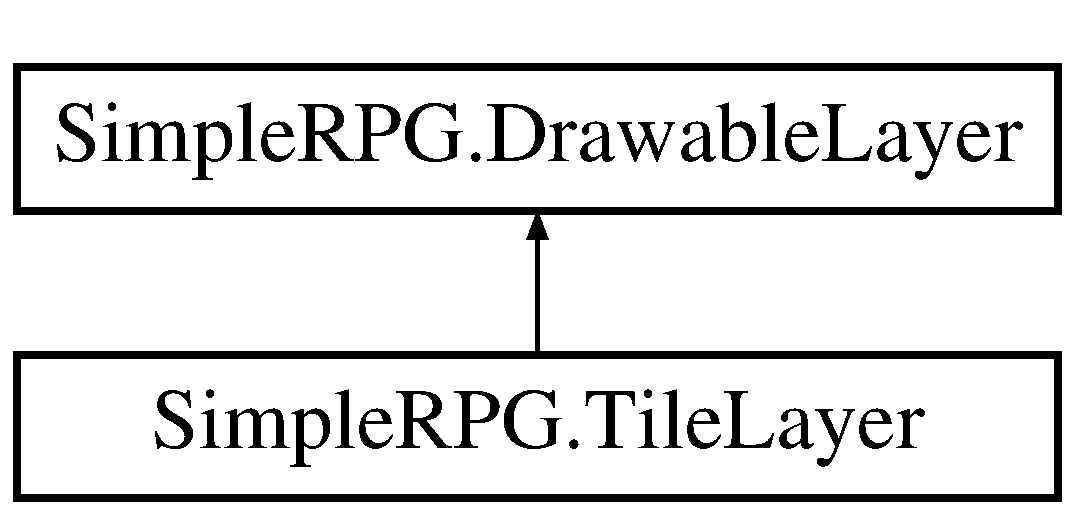
\includegraphics[height=2.000000cm]{class_simple_r_p_g_1_1_tile_layer}
\end{center}
\end{figure}
\subsection*{Public Member Functions}
\begin{DoxyCompactItemize}
\item 
\hypertarget{class_simple_r_p_g_1_1_tile_layer_ace9183fa596c86f2df4a83014ca950f0}{{\bfseries Tile\-Layer} (Game game, string req\-Name, Texture2\-D req\-Texture, int req\-Width, int req\-Height, int req\-Tiles\-Per\-Row, int req\-Tile\-Size)}\label{class_simple_r_p_g_1_1_tile_layer_ace9183fa596c86f2df4a83014ca950f0}

\item 
\hypertarget{class_simple_r_p_g_1_1_tile_layer_a7cc0ae37cfbbc7dc82615bc6c63bf020}{\hyperlink{class_simple_r_p_g_1_1_tile}{Tile}\mbox{[},\mbox{]} {\bfseries get\-Tiles} ()}\label{class_simple_r_p_g_1_1_tile_layer_a7cc0ae37cfbbc7dc82615bc6c63bf020}

\item 
\hypertarget{class_simple_r_p_g_1_1_tile_layer_a8cac5f0cde30090519d897e526a3f57e}{\hyperlink{class_simple_r_p_g_1_1_tile}{Tile} {\bfseries get\-Tile} (int x, int y)}\label{class_simple_r_p_g_1_1_tile_layer_a8cac5f0cde30090519d897e526a3f57e}

\item 
\hypertarget{class_simple_r_p_g_1_1_tile_layer_a5e79fc6d88c3e907eedad7737c9c4e7e}{override \hyperlink{namespace_simple_r_p_g_a5f1ec21e7f4e36278a6cedd38c51e650}{Passability} {\bfseries get\-Passability} (int x, int y)}\label{class_simple_r_p_g_1_1_tile_layer_a5e79fc6d88c3e907eedad7737c9c4e7e}

\item 
\hypertarget{class_simple_r_p_g_1_1_tile_layer_a559edc2f802575814d4e3d762023b878}{override void {\bfseries draw} (Sprite\-Batch sprite\-Batch, Point first\-Tile, int tiles\-Across, int tiles\-Down, Point offset, int scale)}\label{class_simple_r_p_g_1_1_tile_layer_a559edc2f802575814d4e3d762023b878}

\item 
\hypertarget{class_simple_r_p_g_1_1_tile_layer_a7671848d8a5937ba5c73bde28a1f2e11}{void {\bfseries tint\-Tile} (int x, int y, Color tint\-Color)}\label{class_simple_r_p_g_1_1_tile_layer_a7671848d8a5937ba5c73bde28a1f2e11}

\item 
\hypertarget{class_simple_r_p_g_1_1_tile_layer_a4dbc526d42d95a5bfd8a5cc04a7cc2f2}{void {\bfseries clear\-Tint} ()}\label{class_simple_r_p_g_1_1_tile_layer_a4dbc526d42d95a5bfd8a5cc04a7cc2f2}

\end{DoxyCompactItemize}
\subsection*{Additional Inherited Members}


The documentation for this class was generated from the following file\-:\begin{DoxyCompactItemize}
\item 
Simple\-R\-P\-G/\-Simple\-R\-P\-G/Tile\-Layer.\-cs\end{DoxyCompactItemize}

\hypertarget{class_simple_r_p_g_1_1_tile_map}{\section{Simple\+R\+P\+G.\+Tile\+Map Class Reference}
\label{class_simple_r_p_g_1_1_tile_map}\index{Simple\+R\+P\+G.\+Tile\+Map@{Simple\+R\+P\+G.\+Tile\+Map}}
}
Inheritance diagram for Simple\+R\+P\+G.\+Tile\+Map\+:\begin{figure}[H]
\begin{center}
\leavevmode
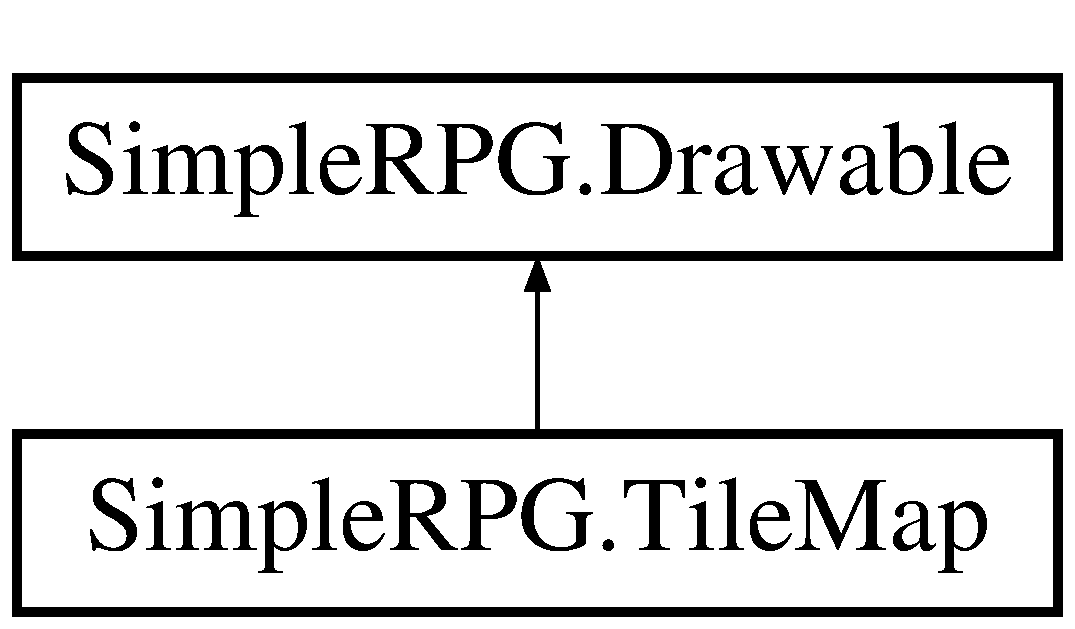
\includegraphics[height=2.000000cm]{class_simple_r_p_g_1_1_tile_map}
\end{center}
\end{figure}
\subsection*{Public Member Functions}
\begin{DoxyCompactItemize}
\item 
\hypertarget{class_simple_r_p_g_1_1_tile_map_aff7e26a8eba6574dc7e44365e0f80116}{{\bfseries Tile\+Map} (Game game, string filename)}\label{class_simple_r_p_g_1_1_tile_map_aff7e26a8eba6574dc7e44365e0f80116}

\item 
\hypertarget{class_simple_r_p_g_1_1_tile_map_af2fe2bc52a70e738c8f0f7fc822d990a}{void {\bfseries update} ()}\label{class_simple_r_p_g_1_1_tile_map_af2fe2bc52a70e738c8f0f7fc822d990a}

\item 
\hypertarget{class_simple_r_p_g_1_1_tile_map_a27f6d71982a60c58caf00cd909169024}{void {\bfseries draw} (Sprite\+Batch sprite\+Batch, Point first\+Tile, int tiles\+Across, int tiles\+Down, Point offset)}\label{class_simple_r_p_g_1_1_tile_map_a27f6d71982a60c58caf00cd909169024}

\item 
\hypertarget{class_simple_r_p_g_1_1_tile_map_aaf5d4d165283c58cce31ebf20bedbb74}{void {\bfseries draw} (Sprite\+Batch sprite\+Batch, Point first\+Tile, int tiles\+Across, int tiles\+Down, Point offset, int scale)}\label{class_simple_r_p_g_1_1_tile_map_aaf5d4d165283c58cce31ebf20bedbb74}

\item 
\hypertarget{class_simple_r_p_g_1_1_tile_map_a3b9d0342243c91c45a8cd4017131019b}{void {\bfseries add\+Object} (\hyperlink{class_simple_r_p_g_1_1_map_object}{Map\+Object} to\+Add)}\label{class_simple_r_p_g_1_1_tile_map_a3b9d0342243c91c45a8cd4017131019b}

\item 
\hypertarget{class_simple_r_p_g_1_1_tile_map_afdecb3d7dc11c14cb87efaac3245d581}{void {\bfseries set\+Opacity} (float value)}\label{class_simple_r_p_g_1_1_tile_map_afdecb3d7dc11c14cb87efaac3245d581}

\item 
\hypertarget{class_simple_r_p_g_1_1_tile_map_a8aee7054993b88b1f0f668a88b3879df}{int {\bfseries get\+Width} ()}\label{class_simple_r_p_g_1_1_tile_map_a8aee7054993b88b1f0f668a88b3879df}

\item 
\hypertarget{class_simple_r_p_g_1_1_tile_map_a021ebfc7b0614b0af61d3a576e421b50}{int {\bfseries get\+Height} ()}\label{class_simple_r_p_g_1_1_tile_map_a021ebfc7b0614b0af61d3a576e421b50}

\item 
\hypertarget{class_simple_r_p_g_1_1_tile_map_aff60bd6ac7270eaaed3e8a56f65908a0}{int {\bfseries get\+Tile\+Size} ()}\label{class_simple_r_p_g_1_1_tile_map_aff60bd6ac7270eaaed3e8a56f65908a0}

\item 
\hypertarget{class_simple_r_p_g_1_1_tile_map_aae945859439ba8cfacde7e4fa2e66e3d}{bool {\bfseries get\+Passability} (int x, int y)}\label{class_simple_r_p_g_1_1_tile_map_aae945859439ba8cfacde7e4fa2e66e3d}

\end{DoxyCompactItemize}
\subsection*{Additional Inherited Members}


The documentation for this class was generated from the following file\+:\begin{DoxyCompactItemize}
\item 
D\+:/\+Dropbox/\+Simple\+R\+P\+G/\+Simple\+R\+P\+G/\+Simple\+R\+P\+G/Tile\+Map.\+cs\end{DoxyCompactItemize}

\hypertarget{class_simple_r_p_g_1_1_states_1_1_use_item_state}{\section{Simple\-R\-P\-G.\-States.\-Use\-Item\-State Class Reference}
\label{class_simple_r_p_g_1_1_states_1_1_use_item_state}\index{Simple\-R\-P\-G.\-States.\-Use\-Item\-State@{Simple\-R\-P\-G.\-States.\-Use\-Item\-State}}
}
Inheritance diagram for Simple\-R\-P\-G.\-States.\-Use\-Item\-State\-:\begin{figure}[H]
\begin{center}
\leavevmode
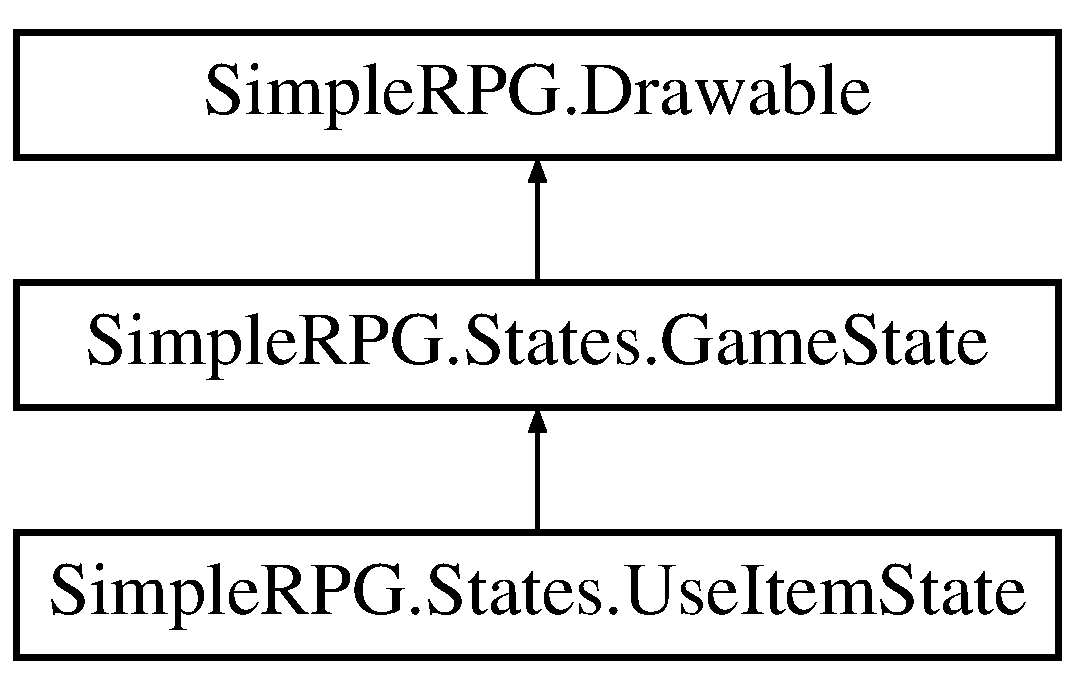
\includegraphics[height=3.000000cm]{class_simple_r_p_g_1_1_states_1_1_use_item_state}
\end{center}
\end{figure}
\subsection*{Public Member Functions}
\begin{DoxyCompactItemize}
\item 
\hypertarget{class_simple_r_p_g_1_1_states_1_1_use_item_state_a11bf3becbf4d48248e00d04c6d44d467}{{\bfseries Use\-Item\-State} (\hyperlink{class_simple_r_p_g_1_1_game1}{Game1} game, \hyperlink{class_simple_r_p_g_1_1_states_1_1_game_state}{Game\-State} parent, \hyperlink{class_simple_r_p_g_1_1_states_1_1_state_manager}{State\-Manager} manager, Point window\-Position, \hyperlink{class_simple_r_p_g_1_1_items_1_1_item}{Item} item)}\label{class_simple_r_p_g_1_1_states_1_1_use_item_state_a11bf3becbf4d48248e00d04c6d44d467}

\item 
\hypertarget{class_simple_r_p_g_1_1_states_1_1_use_item_state_a5d99e92a08bc1407c045e1e5ab37f8b6}{override void {\bfseries draw} (Sprite\-Batch sprite\-Batch)}\label{class_simple_r_p_g_1_1_states_1_1_use_item_state_a5d99e92a08bc1407c045e1e5ab37f8b6}

\item 
\hypertarget{class_simple_r_p_g_1_1_states_1_1_use_item_state_ad385afabb54275c9163ae4a9f69c8145}{override void {\bfseries update} ()}\label{class_simple_r_p_g_1_1_states_1_1_use_item_state_ad385afabb54275c9163ae4a9f69c8145}

\item 
\hypertarget{class_simple_r_p_g_1_1_states_1_1_use_item_state_ae999153e8804e12bb0f9b9234730e498}{override void {\bfseries pass\-Data} (\hyperlink{class_simple_r_p_g_1_1_states_1_1_game_state}{Game\-State} sender, object data)}\label{class_simple_r_p_g_1_1_states_1_1_use_item_state_ae999153e8804e12bb0f9b9234730e498}

\item 
\hypertarget{class_simple_r_p_g_1_1_states_1_1_use_item_state_a8534195016da045a609c6ac0c0285adf}{void {\bfseries set\-Window\-Position} (Point new\-Pos)}\label{class_simple_r_p_g_1_1_states_1_1_use_item_state_a8534195016da045a609c6ac0c0285adf}

\end{DoxyCompactItemize}
\subsection*{Protected Member Functions}
\begin{DoxyCompactItemize}
\item 
virtual void \hyperlink{class_simple_r_p_g_1_1_states_1_1_use_item_state_a1b5489d92cced85b8185d1b98ad06363}{use\-Item} ()
\begin{DoxyCompactList}\small\item\em Called when the selected item is to be used \end{DoxyCompactList}\end{DoxyCompactItemize}
\subsection*{Protected Attributes}
\begin{DoxyCompactItemize}
\item 
\hypertarget{class_simple_r_p_g_1_1_states_1_1_use_item_state_ab5539431d2b7e06ef317fc3b6c78307b}{\hyperlink{class_simple_r_p_g_1_1_windows_1_1_use_item_window}{Use\-Item\-Window} {\bfseries item\-Window}}\label{class_simple_r_p_g_1_1_states_1_1_use_item_state_ab5539431d2b7e06ef317fc3b6c78307b}

\item 
\hypertarget{class_simple_r_p_g_1_1_states_1_1_use_item_state_a296de2ddaf55d62af61c3ccaeb996292}{\hyperlink{class_simple_r_p_g_1_1_items_1_1_usable_item}{Usable\-Item} {\bfseries to\-Use}}\label{class_simple_r_p_g_1_1_states_1_1_use_item_state_a296de2ddaf55d62af61c3ccaeb996292}

\end{DoxyCompactItemize}


\subsection{Member Function Documentation}
\hypertarget{class_simple_r_p_g_1_1_states_1_1_use_item_state_a1b5489d92cced85b8185d1b98ad06363}{\index{Simple\-R\-P\-G\-::\-States\-::\-Use\-Item\-State@{Simple\-R\-P\-G\-::\-States\-::\-Use\-Item\-State}!use\-Item@{use\-Item}}
\index{use\-Item@{use\-Item}!SimpleRPG::States::UseItemState@{Simple\-R\-P\-G\-::\-States\-::\-Use\-Item\-State}}
\subsubsection[{use\-Item}]{\setlength{\rightskip}{0pt plus 5cm}virtual void Simple\-R\-P\-G.\-States.\-Use\-Item\-State.\-use\-Item (
\begin{DoxyParamCaption}
{}
\end{DoxyParamCaption}
)\hspace{0.3cm}{\ttfamily [inline]}, {\ttfamily [protected]}, {\ttfamily [virtual]}}}\label{class_simple_r_p_g_1_1_states_1_1_use_item_state_a1b5489d92cced85b8185d1b98ad06363}


Called when the selected item is to be used 



The documentation for this class was generated from the following file\-:\begin{DoxyCompactItemize}
\item 
Simple\-R\-P\-G/\-Simple\-R\-P\-G/\-States/Use\-Item\-State.\-cs\end{DoxyCompactItemize}

\hypertarget{class_simple_r_p_g_1_1_windows_1_1_use_item_window}{\section{Simple\+R\+P\+G.\+Windows.\+Use\+Item\+Window Class Reference}
\label{class_simple_r_p_g_1_1_windows_1_1_use_item_window}\index{Simple\+R\+P\+G.\+Windows.\+Use\+Item\+Window@{Simple\+R\+P\+G.\+Windows.\+Use\+Item\+Window}}
}
Inheritance diagram for Simple\+R\+P\+G.\+Windows.\+Use\+Item\+Window\+:\begin{figure}[H]
\begin{center}
\leavevmode
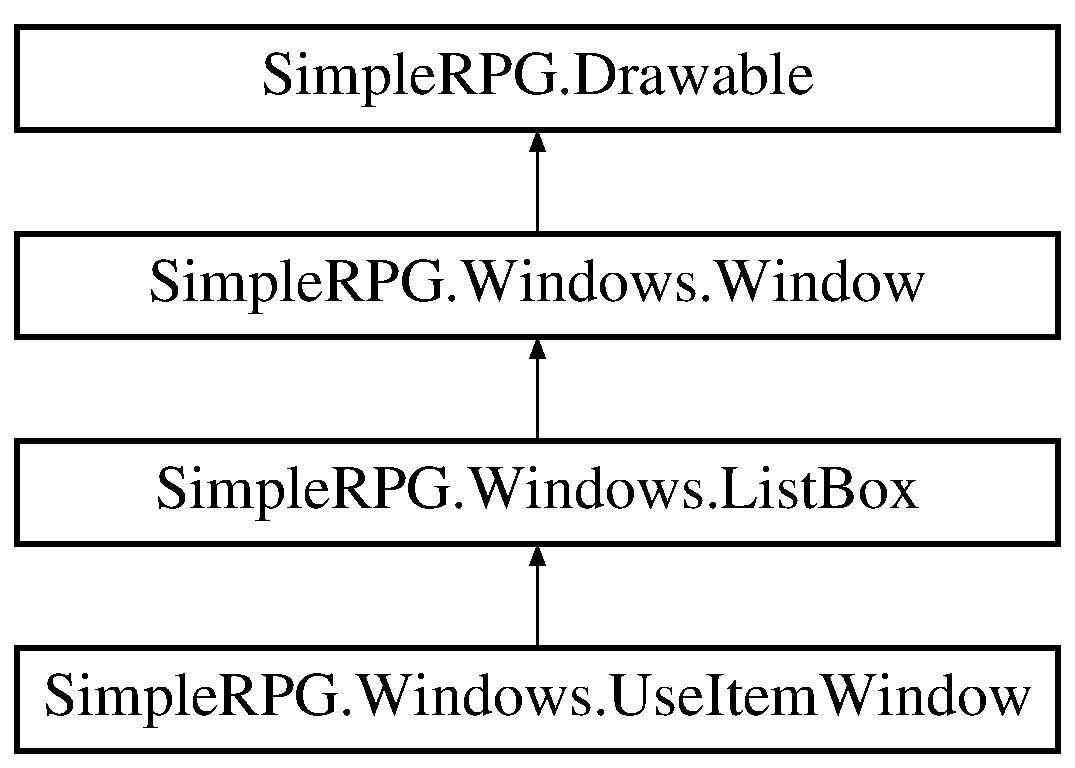
\includegraphics[height=4.000000cm]{class_simple_r_p_g_1_1_windows_1_1_use_item_window}
\end{center}
\end{figure}
\subsection*{Public Member Functions}
\begin{DoxyCompactItemize}
\item 
\hypertarget{class_simple_r_p_g_1_1_windows_1_1_use_item_window_a4eba542441bee99f975409f2d39ccfdd}{{\bfseries Use\+Item\+Window} (\hyperlink{class_simple_r_p_g_1_1_game1}{Game1} game, Point req\+Position)}\label{class_simple_r_p_g_1_1_windows_1_1_use_item_window_a4eba542441bee99f975409f2d39ccfdd}

\end{DoxyCompactItemize}
\subsection*{Additional Inherited Members}


The documentation for this class was generated from the following file\+:\begin{DoxyCompactItemize}
\item 
D\+:/\+Dropbox/\+Simple\+R\+P\+G/\+Simple\+R\+P\+G/\+Simple\+R\+P\+G/\+Windows/Use\+Item\+Window.\+cs\end{DoxyCompactItemize}

\hypertarget{class_simple_r_p_g_1_1_windows_1_1_window}{\section{Simple\+R\+P\+G.\+Windows.\+Window Class Reference}
\label{class_simple_r_p_g_1_1_windows_1_1_window}\index{Simple\+R\+P\+G.\+Windows.\+Window@{Simple\+R\+P\+G.\+Windows.\+Window}}
}
Inheritance diagram for Simple\+R\+P\+G.\+Windows.\+Window\+:\begin{figure}[H]
\begin{center}
\leavevmode
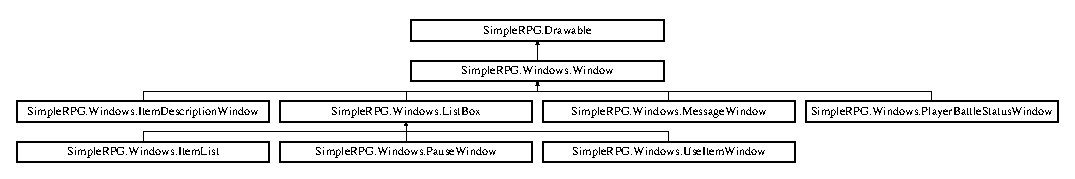
\includegraphics[height=1.958042cm]{class_simple_r_p_g_1_1_windows_1_1_window}
\end{center}
\end{figure}
\subsection*{Public Member Functions}
\begin{DoxyCompactItemize}
\item 
\hypertarget{class_simple_r_p_g_1_1_windows_1_1_window_a77106c03483ec65f3b86d1480f12c5f2}{{\bfseries Window} (\hyperlink{class_simple_r_p_g_1_1_game1}{Game1} game, Point req\+Position, int req\+Width, int req\+Height, string windowskin)}\label{class_simple_r_p_g_1_1_windows_1_1_window_a77106c03483ec65f3b86d1480f12c5f2}

\item 
\hypertarget{class_simple_r_p_g_1_1_windows_1_1_window_a341437b329d28975706528c71edb846f}{override void {\bfseries update} ()}\label{class_simple_r_p_g_1_1_windows_1_1_window_a341437b329d28975706528c71edb846f}

\item 
\hypertarget{class_simple_r_p_g_1_1_windows_1_1_window_ab004ffc0a399c5185085834457f22f0a}{virtual void {\bfseries draw} (Sprite\+Batch sprite\+Batch)}\label{class_simple_r_p_g_1_1_windows_1_1_window_ab004ffc0a399c5185085834457f22f0a}

\item 
\hypertarget{class_simple_r_p_g_1_1_windows_1_1_window_a83b744056d9d1eb19942c265fe2d6c2c}{Point {\bfseries get\+Position} ()}\label{class_simple_r_p_g_1_1_windows_1_1_window_a83b744056d9d1eb19942c265fe2d6c2c}

\item 
\hypertarget{class_simple_r_p_g_1_1_windows_1_1_window_a0d512f21515452828d606cb51a7116f9}{int {\bfseries get\+Width} ()}\label{class_simple_r_p_g_1_1_windows_1_1_window_a0d512f21515452828d606cb51a7116f9}

\item 
\hypertarget{class_simple_r_p_g_1_1_windows_1_1_window_af56ab67ac135f8cf5d664507b1e5c3d9}{int {\bfseries get\+Height} ()}\label{class_simple_r_p_g_1_1_windows_1_1_window_af56ab67ac135f8cf5d664507b1e5c3d9}

\end{DoxyCompactItemize}
\subsection*{Protected Attributes}
\begin{DoxyCompactItemize}
\item 
\hypertarget{class_simple_r_p_g_1_1_windows_1_1_window_ad22a60b848c0e7118745c529f1ccd702}{int {\bfseries width}}\label{class_simple_r_p_g_1_1_windows_1_1_window_ad22a60b848c0e7118745c529f1ccd702}

\item 
\hypertarget{class_simple_r_p_g_1_1_windows_1_1_window_aae95399621f4410ffbef8f869f72f521}{Point {\bfseries location}}\label{class_simple_r_p_g_1_1_windows_1_1_window_aae95399621f4410ffbef8f869f72f521}

\item 
\hypertarget{class_simple_r_p_g_1_1_windows_1_1_window_a44a13f36ab800ee3d2d9aa2f36506fd0}{Texture2\+D {\bfseries skin}}\label{class_simple_r_p_g_1_1_windows_1_1_window_a44a13f36ab800ee3d2d9aa2f36506fd0}

\item 
\hypertarget{class_simple_r_p_g_1_1_windows_1_1_window_aaf2e3e1c8b30e500ce4cebf06f8917ea}{Sprite\+Font {\bfseries font}}\label{class_simple_r_p_g_1_1_windows_1_1_window_aaf2e3e1c8b30e500ce4cebf06f8917ea}

\item 
\hypertarget{class_simple_r_p_g_1_1_windows_1_1_window_ae684d28fca3747c4785d025504284d24}{\hyperlink{class_simple_r_p_g_1_1_game1}{Game1} {\bfseries game\+Ref}}\label{class_simple_r_p_g_1_1_windows_1_1_window_ae684d28fca3747c4785d025504284d24}

\item 
\hypertarget{class_simple_r_p_g_1_1_windows_1_1_window_a0e75e20f1345fcce9df4dddbaefe054c}{Color {\bfseries text\+Color}}\label{class_simple_r_p_g_1_1_windows_1_1_window_a0e75e20f1345fcce9df4dddbaefe054c}

\end{DoxyCompactItemize}


The documentation for this class was generated from the following file\+:\begin{DoxyCompactItemize}
\item 
D\+:/\+Dropbox/\+Simple\+R\+P\+G/\+Simple\+R\+P\+G/\+Simple\+R\+P\+G/\+Windows/Window.\+cs\end{DoxyCompactItemize}

%--- End generated contents ---

% Index
\newpage
\phantomsection
\addcontentsline{toc}{chapter}{Index}
\printindex

\end{document}
